%!TEX TS-program = xelatex
\documentclass[10pt, compress]{beamer}

\usetheme[usetitleprogressbar]{m}

\usepackage{booktabs}
\usepackage{tikz}
\usepackage{dcolumn}
\usepackage[scale=2]{ccicons}
\usepackage{color}

\graphicspath{{Graphics/}}

\title[Tensors]{\textsc{Relax, Tensors Are Here...with Exogenous Covariates}}
\author[Hoff, Minhas, \& Ward]{Peter D. Hoff, Shahryar Minhas, \& Michael D. Ward} 
\date{\today}

\begin{document}
\frame{\titlepage}

%%%%%%%%%%%%%%%%%%%%%%%%%%%%%%%%%%%%%%%%%%%%%%%%%%%%%%%%%%%%
\frame
{
  \frametitle{Model Specification}
  \vspace{-5mm}
  \begin{itemize}
  \item Dependent variables: Log(Exports) and Stdzed(Material Conflict). 
  \item Direct ($i$), reciprocal ($ji$) and transitive ($ijk$) 1 month lags of these included as IVs.
  \item Exogenous Covariates:
    \begin{itemize}
    \item Number of Preferential Trade Agreements (PTA) between $i$ and $j$ (this is an undirected, yearly level variable). Direct and transitive version of this variable included as covariates.
    \item Presence of a defensive alliance relationship between $i$ and $j$ (undirected, yearly level). Direct and transitive versions.
    \item Centroid distance between $i$ and $j$ (directed). Direct version.
    \item Polity, monthly level variable. Polity of sender included.
    \item Log(GDP), yearly level variable but imputed at the monthly level. GDP of sender.
    \item Log(Population), yearly level variable but imputed at the monthly level. Population of sender.
    \item Log(Total Exports to any country), monthly level variable. Exports of sender.
    \end{itemize}
  \end{itemize}    
} 
%%%%%%%%%%%%%%%%%%%%%%%%%%%%%%%%%%%%%%%%%%%%%%%%%%%%%%%%%%%%

%%%%%%%%%%%%%%%%%%%%%%%%%%%%%%%%%%%%%%%%%%%%%%%%%%%%%%%%%%%%
\frame
{
  \frametitle{Sample \& Data}
  \begin{itemize}
  \item  Our sample is comprised of 161 countries over the period of March 2001 to December 2014
  \item Data sources:
  \begin{itemize}
    \item Exports: \href{http://data.imf.org/?sk=8aa6eb7c-598b-4d3b-82f4-adab95d23145&dsId=DS_1414779485682}{\textcolor{blue}{IMF Direction of Trade Statistics}}
    \item Material Conflict: ICEWS
    \item PTA: \href{http://www.designoftradeagreements.org/}{\textcolor{blue}{Design of Trade Agreements Database}}
    \item Alliance: \href{http://www.correlatesofwar.org/news/alliances-data-set-v4-1-available-1}{\textcolor{blue}{Correlates of War}}
    \item Distance: \href{http://nils.weidmann.ws/projects/cshapes}{\textcolor{blue}{cshapes}}
    \item Polity: \href{http://www.systemicpeace.org/polity/polity4.htm}{\textcolor{blue}{Polity IV Project}}
    \item GDP, Population: \href{https://www.imf.org/external/pubs/ft/weo/2014/02/weodata/index.aspx}{\textcolor{blue}{IMF World Economic Outlook Database}}
  \end{itemize}
  \end{itemize}    
} 
%%%%%%%%%%%%%%%%%%%%%%%%%%%%%%%%%%%%%%%%%%%%%%%%%%%%%%%%%%%%

%%%%%%%%%%%%%%%%%%%%%%%%%%%%%%%%%%%%%%%%%%%%%%%%%%%%%%%%%%%%
\frame
{
  \frametitle{Modeling Approach}
  \begin{itemize}
  \item Multilinear tensor regression framework
  \item MCMC run for 1300 iterations with first 600 used as burn-in\footnote{Using this many datapoints takes time the MCMC will keep running for another 3700 iterations so these results are preliminary, but trace plots at the end of this pdf look stable after 600 iterations}
  \item The model has the following form:
  \begin{align*}
  \textbf{Y} = \textbf{X} \times \{\boldsymbol{\beta_{1}}, \boldsymbol{\beta_{2}}, \boldsymbol{\beta_{3}} \} + \textbf{E}
  \end{align*}
  \item \textbf{Y} is a $161 \times 161 \times 2 \times 165$ array
  \item \textbf{X} is a $161 \times 161 \times 13 \times 165$ array, where each of the 13 variables is lagged by one month
  \end{itemize}    
} 
%%%%%%%%%%%%%%%%%%%%%%%%%%%%%%%%%%%%%%%%%%%%%%%%%%%%%%%%%%%%

%%%%%%%%%%%%%%%%%%%%%%%%%%%%%%%%%%%%%%%%%%%%%%%%%%%%%%%%%%%%
\frame
{
\frametitle{$\boldsymbol{\beta_{1}}$ \& $\boldsymbol{\beta_{2}}$, Sig. $+$ shown, $\alpha = 0.01$}
  \vspace{-15mm}
  \begin{figure}[ht]
  \centering
    \begin{tabular}{c}
      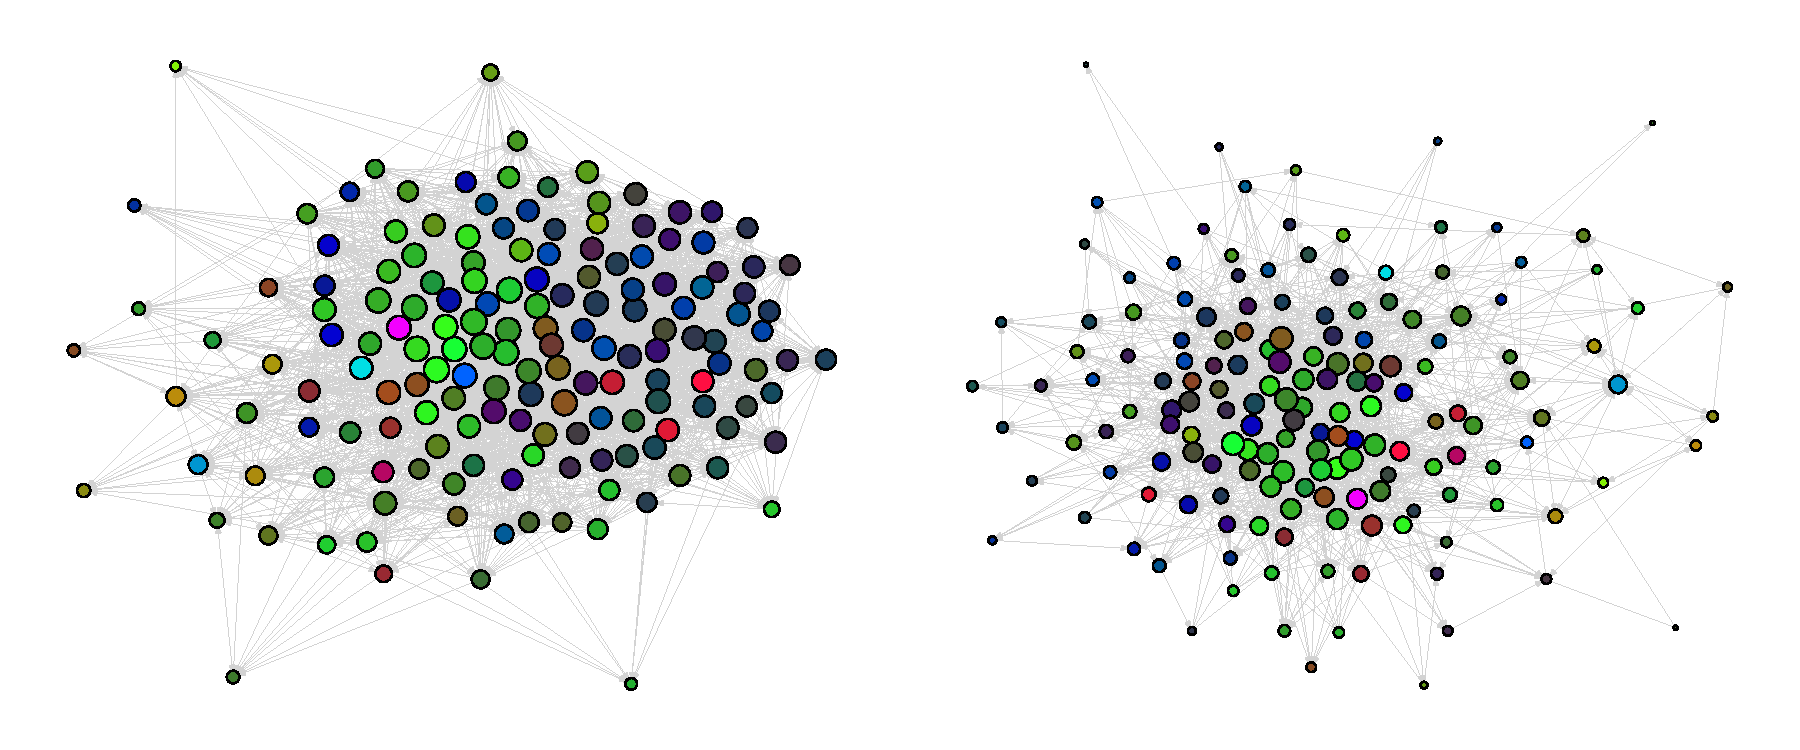
\includegraphics[width=1\textwidth]{net.pdf} \\
      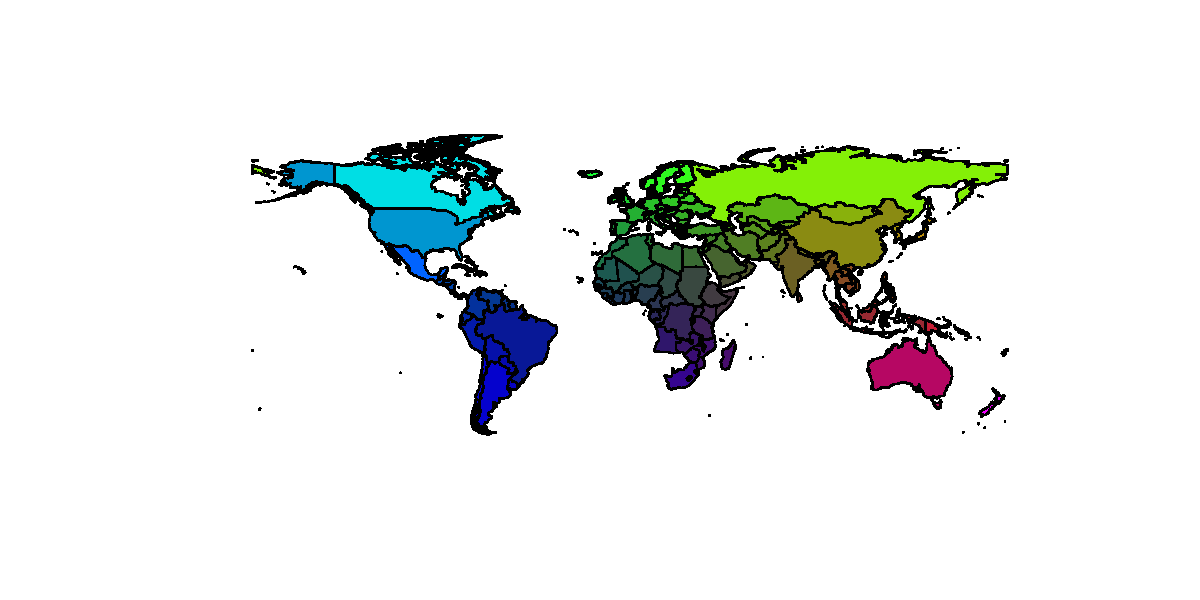
\includegraphics[width=.9\textwidth]{map.pdf}
    \end{tabular}
  \end{figure}
}
%%%%%%%%%%%%%%%%%%%%%%%%%%%%%%%%%%%%%%%%%%%%%%%%%%%%%%%%%%%%

%%%%%%%%%%%%%%%%%%%%%%%%%%%%%%%%%%%%%%%%%%%%%%%%%%%%%%%%%%%%
\frame
{
\frametitle{$\boldsymbol{\beta_{3}}$}
  \centering
  \resizebox{1\textwidth}{!}{% Created by tikzDevice version 0.8.1 on 2015-06-28 20:26:01
% !TEX encoding = UTF-8 Unicode
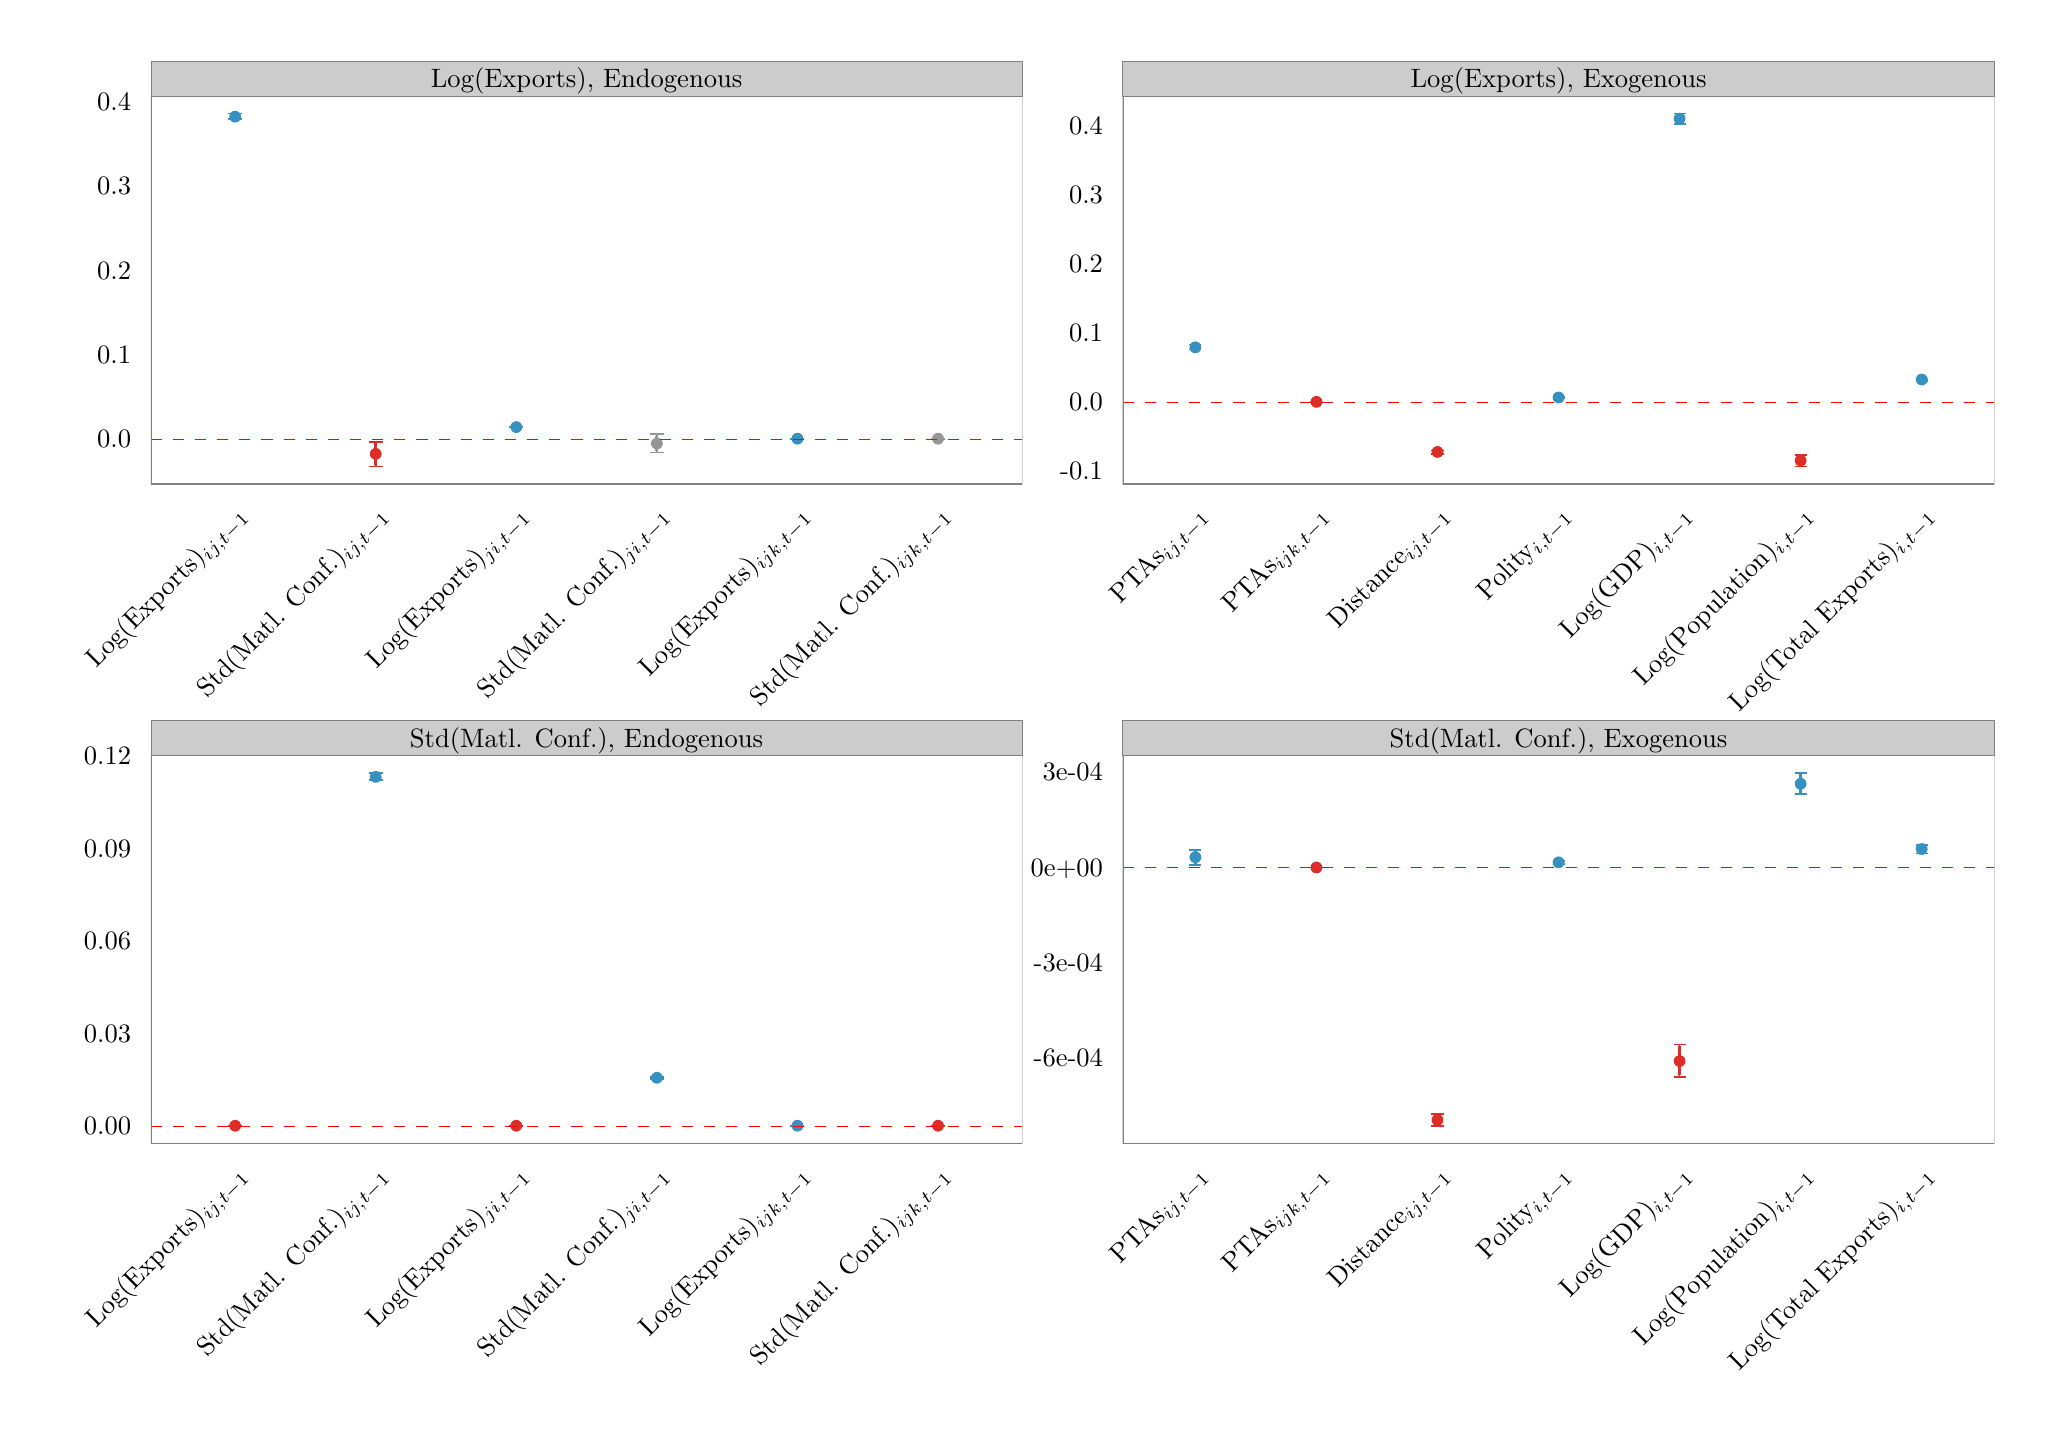
\begin{tikzpicture}[x=1pt,y=1pt]
\definecolor{fillColor}{RGB}{255,255,255}
\path[use as bounding box,fill=fillColor,fill opacity=0.00] (0,0) rectangle (722.70,505.89);
\begin{scope}
\path[clip] (  0.00,  0.00) rectangle (722.70,505.89);
\definecolor{drawColor}{RGB}{255,255,255}
\definecolor{fillColor}{RGB}{255,255,255}

\path[draw=drawColor,line width= 0.6pt,line join=round,line cap=round,fill=fillColor] (  0.00,  0.00) rectangle (722.70,505.89);
\end{scope}
\begin{scope}
\path[clip] ( 44.49,340.99) rectangle (359.44,481.21);
\definecolor{fillColor}{RGB}{54,144,192}

\path[fill=fillColor] ( 74.97,473.73) circle (  2.13);
\definecolor{fillColor}{RGB}{222,45,38}

\path[fill=fillColor] (125.77,351.89) circle (  2.13);
\definecolor{fillColor}{RGB}{54,144,192}

\path[fill=fillColor] (176.56,361.55) circle (  2.13);
\definecolor{fillColor}{gray}{0.59}

\path[fill=fillColor] (227.36,355.63) circle (  2.13);
\definecolor{fillColor}{RGB}{54,144,192}

\path[fill=fillColor] (278.16,357.36) circle (  2.13);
\definecolor{fillColor}{gray}{0.59}

\path[fill=fillColor] (328.96,357.36) circle (  2.13);
\definecolor{drawColor}{RGB}{54,144,192}

\path[draw=drawColor,draw opacity=0.30,line width= 0.3pt,line join=round] ( 74.97,472.79) -- ( 74.97,474.84);
\definecolor{drawColor}{RGB}{222,45,38}

\path[draw=drawColor,draw opacity=0.30,line width= 0.3pt,line join=round] (125.77,347.36) -- (125.77,356.18);
\definecolor{drawColor}{RGB}{54,144,192}

\path[draw=drawColor,draw opacity=0.30,line width= 0.3pt,line join=round] (176.56,361.43) -- (176.56,361.67);
\definecolor{drawColor}{RGB}{150,150,150}

\path[draw=drawColor,draw opacity=0.30,line width= 0.3pt,line join=round] (227.36,352.41) -- (227.36,359.04);
\definecolor{drawColor}{RGB}{54,144,192}

\path[draw=drawColor,draw opacity=0.30,line width= 0.3pt,line join=round] (278.16,357.36) -- (278.16,357.36);
\definecolor{drawColor}{RGB}{150,150,150}

\path[draw=drawColor,draw opacity=0.30,line width= 0.3pt,line join=round] (328.96,357.35) -- (328.96,357.37);
\definecolor{drawColor}{RGB}{54,144,192}

\path[draw=drawColor,line width= 1.1pt,line join=round] ( 74.97,472.86) -- ( 74.97,474.75);
\definecolor{drawColor}{RGB}{222,45,38}

\path[draw=drawColor,line width= 1.1pt,line join=round] (125.77,347.76) -- (125.77,355.64);
\definecolor{drawColor}{RGB}{54,144,192}

\path[draw=drawColor,line width= 1.1pt,line join=round] (176.56,361.45) -- (176.56,361.66);
\definecolor{drawColor}{gray}{0.59}

\path[draw=drawColor,line width= 1.1pt,line join=round] (227.36,352.95) -- (227.36,358.31);
\definecolor{drawColor}{RGB}{54,144,192}

\path[draw=drawColor,line width= 1.1pt,line join=round] (278.16,357.36) -- (278.16,357.36);
\definecolor{drawColor}{gray}{0.59}

\path[draw=drawColor,line width= 1.1pt,line join=round] (328.96,357.35) -- (328.96,357.37);
\definecolor{drawColor}{RGB}{54,144,192}

\path[draw=drawColor,line width= 0.6pt,line join=round] ( 72.43,474.84) --
	( 77.51,474.84);

\path[draw=drawColor,line width= 0.6pt,line join=round] ( 74.97,474.84) --
	( 74.97,472.79);

\path[draw=drawColor,line width= 0.6pt,line join=round] ( 72.43,472.79) --
	( 77.51,472.79);
\definecolor{drawColor}{RGB}{222,45,38}

\path[draw=drawColor,line width= 0.6pt,line join=round] (123.23,356.18) --
	(128.31,356.18);

\path[draw=drawColor,line width= 0.6pt,line join=round] (125.77,356.18) --
	(125.77,347.36);

\path[draw=drawColor,line width= 0.6pt,line join=round] (123.23,347.36) --
	(128.31,347.36);
\definecolor{drawColor}{RGB}{54,144,192}

\path[draw=drawColor,line width= 0.6pt,line join=round] (174.03,361.67) --
	(179.10,361.67);

\path[draw=drawColor,line width= 0.6pt,line join=round] (176.56,361.67) --
	(176.56,361.43);

\path[draw=drawColor,line width= 0.6pt,line join=round] (174.03,361.43) --
	(179.10,361.43);
\definecolor{drawColor}{gray}{0.59}

\path[draw=drawColor,line width= 0.6pt,line join=round] (224.82,359.04) --
	(229.90,359.04);

\path[draw=drawColor,line width= 0.6pt,line join=round] (227.36,359.04) --
	(227.36,352.41);

\path[draw=drawColor,line width= 0.6pt,line join=round] (224.82,352.41) --
	(229.90,352.41);
\definecolor{drawColor}{RGB}{54,144,192}

\path[draw=drawColor,line width= 0.6pt,line join=round] (275.62,357.36) --
	(280.70,357.36);

\path[draw=drawColor,line width= 0.6pt,line join=round] (278.16,357.36) --
	(278.16,357.36);

\path[draw=drawColor,line width= 0.6pt,line join=round] (275.62,357.36) --
	(280.70,357.36);
\definecolor{drawColor}{gray}{0.59}

\path[draw=drawColor,line width= 0.6pt,line join=round] (326.42,357.37) --
	(331.50,357.37);

\path[draw=drawColor,line width= 0.6pt,line join=round] (328.96,357.37) --
	(328.96,357.35);

\path[draw=drawColor,line width= 0.6pt,line join=round] (326.42,357.35) --
	(331.50,357.35);
\definecolor{drawColor}{RGB}{255,0,0}

\path[draw=drawColor,line width= 0.1pt,dash pattern=on 4pt off 4pt ,line join=round] ( 44.49,357.35) -- (359.44,357.35);
\definecolor{drawColor}{gray}{0.50}

\path[draw=drawColor,line width= 0.6pt,line join=round,line cap=round] ( 44.49,340.99) rectangle (359.44,481.21);
\end{scope}
\begin{scope}
\path[clip] (395.70,340.99) rectangle (710.66,481.21);
\definecolor{fillColor}{RGB}{54,144,192}

\path[fill=fillColor] (421.94,390.38) circle (  2.13);
\definecolor{fillColor}{RGB}{222,45,38}

\path[fill=fillColor] (465.69,370.67) circle (  2.13);

\path[fill=fillColor] (509.43,352.56) circle (  2.13);
\definecolor{fillColor}{RGB}{54,144,192}

\path[fill=fillColor] (553.18,372.27) circle (  2.13);

\path[fill=fillColor] (596.92,473.02) circle (  2.13);
\definecolor{fillColor}{RGB}{222,45,38}

\path[fill=fillColor] (640.66,349.47) circle (  2.13);
\definecolor{fillColor}{RGB}{54,144,192}

\path[fill=fillColor] (684.41,378.74) circle (  2.13);
\definecolor{drawColor}{RGB}{54,144,192}

\path[draw=drawColor,draw opacity=0.30,line width= 0.3pt,line join=round] (421.94,389.61) -- (421.94,391.34);
\definecolor{drawColor}{RGB}{222,45,38}

\path[draw=drawColor,draw opacity=0.30,line width= 0.3pt,line join=round] (465.69,370.66) -- (465.69,370.68);

\path[draw=drawColor,draw opacity=0.30,line width= 0.3pt,line join=round] (509.43,351.89) -- (509.43,353.15);
\definecolor{drawColor}{RGB}{54,144,192}

\path[draw=drawColor,draw opacity=0.30,line width= 0.3pt,line join=round] (553.18,372.13) -- (553.18,372.46);

\path[draw=drawColor,draw opacity=0.30,line width= 0.3pt,line join=round] (596.92,471.02) -- (596.92,474.84);
\definecolor{drawColor}{RGB}{222,45,38}

\path[draw=drawColor,draw opacity=0.30,line width= 0.3pt,line join=round] (640.66,347.36) -- (640.66,351.51);
\definecolor{drawColor}{RGB}{54,144,192}

\path[draw=drawColor,draw opacity=0.30,line width= 0.3pt,line join=round] (684.41,378.24) -- (684.41,379.14);
\definecolor{drawColor}{RGB}{54,144,192}

\path[draw=drawColor,line width= 1.1pt,line join=round] (421.94,389.74) -- (421.94,391.19);
\definecolor{drawColor}{RGB}{222,45,38}

\path[draw=drawColor,line width= 1.1pt,line join=round] (465.69,370.66) -- (465.69,370.68);

\path[draw=drawColor,line width= 1.1pt,line join=round] (509.43,352.02) -- (509.43,353.10);
\definecolor{drawColor}{RGB}{54,144,192}

\path[draw=drawColor,line width= 1.1pt,line join=round] (553.18,372.15) -- (553.18,372.40);

\path[draw=drawColor,line width= 1.1pt,line join=round] (596.92,471.12) -- (596.92,474.72);
\definecolor{drawColor}{RGB}{222,45,38}

\path[draw=drawColor,line width= 1.1pt,line join=round] (640.66,347.78) -- (640.66,351.37);
\definecolor{drawColor}{RGB}{54,144,192}

\path[draw=drawColor,line width= 1.1pt,line join=round] (684.41,378.33) -- (684.41,379.08);

\path[draw=drawColor,line width= 0.6pt,line join=round] (419.76,391.34) --
	(424.13,391.34);

\path[draw=drawColor,line width= 0.6pt,line join=round] (421.94,391.34) --
	(421.94,389.61);

\path[draw=drawColor,line width= 0.6pt,line join=round] (419.76,389.61) --
	(424.13,389.61);
\definecolor{drawColor}{RGB}{222,45,38}

\path[draw=drawColor,line width= 0.6pt,line join=round] (463.50,370.68) --
	(467.87,370.68);

\path[draw=drawColor,line width= 0.6pt,line join=round] (465.69,370.68) --
	(465.69,370.66);

\path[draw=drawColor,line width= 0.6pt,line join=round] (463.50,370.66) --
	(467.87,370.66);

\path[draw=drawColor,line width= 0.6pt,line join=round] (507.24,353.15) --
	(511.62,353.15);

\path[draw=drawColor,line width= 0.6pt,line join=round] (509.43,353.15) --
	(509.43,351.89);

\path[draw=drawColor,line width= 0.6pt,line join=round] (507.24,351.89) --
	(511.62,351.89);
\definecolor{drawColor}{RGB}{54,144,192}

\path[draw=drawColor,line width= 0.6pt,line join=round] (550.99,372.46) --
	(555.36,372.46);

\path[draw=drawColor,line width= 0.6pt,line join=round] (553.18,372.46) --
	(553.18,372.13);

\path[draw=drawColor,line width= 0.6pt,line join=round] (550.99,372.13) --
	(555.36,372.13);

\path[draw=drawColor,line width= 0.6pt,line join=round] (594.73,474.84) --
	(599.11,474.84);

\path[draw=drawColor,line width= 0.6pt,line join=round] (596.92,474.84) --
	(596.92,471.02);

\path[draw=drawColor,line width= 0.6pt,line join=round] (594.73,471.02) --
	(599.11,471.02);
\definecolor{drawColor}{RGB}{222,45,38}

\path[draw=drawColor,line width= 0.6pt,line join=round] (638.48,351.51) --
	(642.85,351.51);

\path[draw=drawColor,line width= 0.6pt,line join=round] (640.66,351.51) --
	(640.66,347.36);

\path[draw=drawColor,line width= 0.6pt,line join=round] (638.48,347.36) --
	(642.85,347.36);
\definecolor{drawColor}{RGB}{54,144,192}

\path[draw=drawColor,line width= 0.6pt,line join=round] (682.22,379.14) --
	(686.60,379.14);

\path[draw=drawColor,line width= 0.6pt,line join=round] (684.41,379.14) --
	(684.41,378.24);

\path[draw=drawColor,line width= 0.6pt,line join=round] (682.22,378.24) --
	(686.60,378.24);
\definecolor{drawColor}{RGB}{255,0,0}

\path[draw=drawColor,line width= 0.1pt,dash pattern=on 4pt off 4pt ,line join=round] (395.70,370.74) -- (710.66,370.74);
\definecolor{drawColor}{gray}{0.50}

\path[draw=drawColor,line width= 0.6pt,line join=round,line cap=round] (395.70,340.99) rectangle (710.65,481.21);
\end{scope}
\begin{scope}
\path[clip] ( 44.49,102.71) rectangle (359.44,242.94);
\definecolor{fillColor}{RGB}{222,45,38}

\path[fill=fillColor] ( 74.97,109.09) circle (  2.13);
\definecolor{fillColor}{RGB}{54,144,192}

\path[fill=fillColor] (125.77,235.16) circle (  2.13);
\definecolor{fillColor}{RGB}{222,45,38}

\path[fill=fillColor] (176.56,109.10) circle (  2.13);
\definecolor{fillColor}{RGB}{54,144,192}

\path[fill=fillColor] (227.36,126.43) circle (  2.13);

\path[fill=fillColor] (278.16,109.11) circle (  2.13);
\definecolor{fillColor}{RGB}{222,45,38}

\path[fill=fillColor] (328.96,109.10) circle (  2.13);
\definecolor{drawColor}{RGB}{222,45,38}

\path[draw=drawColor,draw opacity=0.30,line width= 0.3pt,line join=round] ( 74.97,109.09) -- ( 74.97,109.10);
\definecolor{drawColor}{RGB}{54,144,192}

\path[draw=drawColor,draw opacity=0.30,line width= 0.3pt,line join=round] (125.77,233.93) -- (125.77,236.56);
\definecolor{drawColor}{RGB}{222,45,38}

\path[draw=drawColor,draw opacity=0.30,line width= 0.3pt,line join=round] (176.56,109.10) -- (176.56,109.11);
\definecolor{drawColor}{RGB}{54,144,192}

\path[draw=drawColor,draw opacity=0.30,line width= 0.3pt,line join=round] (227.36,126.01) -- (227.36,126.83);

\path[draw=drawColor,draw opacity=0.30,line width= 0.3pt,line join=round] (278.16,109.11) -- (278.16,109.11);
\definecolor{drawColor}{RGB}{222,45,38}

\path[draw=drawColor,draw opacity=0.30,line width= 0.3pt,line join=round] (328.96,109.10) -- (328.96,109.10);
\definecolor{drawColor}{RGB}{222,45,38}

\path[draw=drawColor,line width= 1.1pt,line join=round] ( 74.97,109.09) -- ( 74.97,109.10);
\definecolor{drawColor}{RGB}{54,144,192}

\path[draw=drawColor,line width= 1.1pt,line join=round] (125.77,234.15) -- (125.77,236.40);
\definecolor{drawColor}{RGB}{222,45,38}

\path[draw=drawColor,line width= 1.1pt,line join=round] (176.56,109.10) -- (176.56,109.11);
\definecolor{drawColor}{RGB}{54,144,192}

\path[draw=drawColor,line width= 1.1pt,line join=round] (227.36,126.07) -- (227.36,126.77);

\path[draw=drawColor,line width= 1.1pt,line join=round] (278.16,109.11) -- (278.16,109.11);
\definecolor{drawColor}{RGB}{222,45,38}

\path[draw=drawColor,line width= 1.1pt,line join=round] (328.96,109.10) -- (328.96,109.10);

\path[draw=drawColor,line width= 0.6pt,line join=round] ( 72.43,109.10) --
	( 77.51,109.10);

\path[draw=drawColor,line width= 0.6pt,line join=round] ( 74.97,109.10) --
	( 74.97,109.09);

\path[draw=drawColor,line width= 0.6pt,line join=round] ( 72.43,109.09) --
	( 77.51,109.09);
\definecolor{drawColor}{RGB}{54,144,192}

\path[draw=drawColor,line width= 0.6pt,line join=round] (123.23,236.56) --
	(128.31,236.56);

\path[draw=drawColor,line width= 0.6pt,line join=round] (125.77,236.56) --
	(125.77,233.93);

\path[draw=drawColor,line width= 0.6pt,line join=round] (123.23,233.93) --
	(128.31,233.93);
\definecolor{drawColor}{RGB}{222,45,38}

\path[draw=drawColor,line width= 0.6pt,line join=round] (174.03,109.11) --
	(179.10,109.11);

\path[draw=drawColor,line width= 0.6pt,line join=round] (176.56,109.11) --
	(176.56,109.10);

\path[draw=drawColor,line width= 0.6pt,line join=round] (174.03,109.10) --
	(179.10,109.10);
\definecolor{drawColor}{RGB}{54,144,192}

\path[draw=drawColor,line width= 0.6pt,line join=round] (224.82,126.83) --
	(229.90,126.83);

\path[draw=drawColor,line width= 0.6pt,line join=round] (227.36,126.83) --
	(227.36,126.01);

\path[draw=drawColor,line width= 0.6pt,line join=round] (224.82,126.01) --
	(229.90,126.01);

\path[draw=drawColor,line width= 0.6pt,line join=round] (275.62,109.11) --
	(280.70,109.11);

\path[draw=drawColor,line width= 0.6pt,line join=round] (278.16,109.11) --
	(278.16,109.11);

\path[draw=drawColor,line width= 0.6pt,line join=round] (275.62,109.11) --
	(280.70,109.11);
\definecolor{drawColor}{RGB}{222,45,38}

\path[draw=drawColor,line width= 0.6pt,line join=round] (326.42,109.10) --
	(331.50,109.10);

\path[draw=drawColor,line width= 0.6pt,line join=round] (328.96,109.10) --
	(328.96,109.10);

\path[draw=drawColor,line width= 0.6pt,line join=round] (326.42,109.10) --
	(331.50,109.10);
\definecolor{drawColor}{RGB}{255,0,0}

\path[draw=drawColor,line width= 0.1pt,dash pattern=on 4pt off 4pt ,line join=round] ( 44.49,109.11) -- (359.44,109.11);
\definecolor{drawColor}{gray}{0.50}

\path[draw=drawColor,line width= 0.6pt,line join=round,line cap=round] ( 44.49,102.71) rectangle (359.44,242.94);
\end{scope}
\begin{scope}
\path[clip] (395.70,102.71) rectangle (710.66,242.94);
\definecolor{fillColor}{RGB}{54,144,192}

\path[fill=fillColor] (421.94,206.13) circle (  2.13);
\definecolor{fillColor}{RGB}{222,45,38}

\path[fill=fillColor] (465.69,202.41) circle (  2.13);

\path[fill=fillColor] (509.43,111.18) circle (  2.13);
\definecolor{fillColor}{RGB}{54,144,192}

\path[fill=fillColor] (553.18,204.28) circle (  2.13);
\definecolor{fillColor}{RGB}{222,45,38}

\path[fill=fillColor] (596.92,132.47) circle (  2.13);
\definecolor{fillColor}{RGB}{54,144,192}

\path[fill=fillColor] (640.66,232.67) circle (  2.13);

\path[fill=fillColor] (684.41,209.09) circle (  2.13);
\definecolor{drawColor}{RGB}{54,144,192}

\path[draw=drawColor,draw opacity=0.30,line width= 0.3pt,line join=round] (421.94,203.35) -- (421.94,208.65);
\definecolor{drawColor}{RGB}{222,45,38}

\path[draw=drawColor,draw opacity=0.30,line width= 0.3pt,line join=round] (465.69,202.39) -- (465.69,202.43);

\path[draw=drawColor,draw opacity=0.30,line width= 0.3pt,line join=round] (509.43,109.09) -- (509.43,113.41);
\definecolor{drawColor}{RGB}{54,144,192}

\path[draw=drawColor,draw opacity=0.30,line width= 0.3pt,line join=round] (553.18,203.66) -- (553.18,204.88);
\definecolor{drawColor}{RGB}{222,45,38}

\path[draw=drawColor,draw opacity=0.30,line width= 0.3pt,line join=round] (596.92,126.80) -- (596.92,138.45);
\definecolor{drawColor}{RGB}{54,144,192}

\path[draw=drawColor,draw opacity=0.30,line width= 0.3pt,line join=round] (640.66,229.07) -- (640.66,236.56);

\path[draw=drawColor,draw opacity=0.30,line width= 0.3pt,line join=round] (684.41,207.53) -- (684.41,210.64);
\definecolor{drawColor}{RGB}{54,144,192}

\path[draw=drawColor,line width= 1.1pt,line join=round] (421.94,203.67) -- (421.94,208.33);
\definecolor{drawColor}{RGB}{222,45,38}

\path[draw=drawColor,line width= 1.1pt,line join=round] (465.69,202.39) -- (465.69,202.42);

\path[draw=drawColor,line width= 1.1pt,line join=round] (509.43,109.42) -- (509.43,113.09);
\definecolor{drawColor}{RGB}{54,144,192}

\path[draw=drawColor,line width= 1.1pt,line join=round] (553.18,203.76) -- (553.18,204.79);
\definecolor{drawColor}{RGB}{222,45,38}

\path[draw=drawColor,line width= 1.1pt,line join=round] (596.92,127.40) -- (596.92,137.84);
\definecolor{drawColor}{RGB}{54,144,192}

\path[draw=drawColor,line width= 1.1pt,line join=round] (640.66,229.49) -- (640.66,236.09);

\path[draw=drawColor,line width= 1.1pt,line join=round] (684.41,207.79) -- (684.41,210.49);

\path[draw=drawColor,line width= 0.6pt,line join=round] (419.76,208.65) --
	(424.13,208.65);

\path[draw=drawColor,line width= 0.6pt,line join=round] (421.94,208.65) --
	(421.94,203.35);

\path[draw=drawColor,line width= 0.6pt,line join=round] (419.76,203.35) --
	(424.13,203.35);
\definecolor{drawColor}{RGB}{222,45,38}

\path[draw=drawColor,line width= 0.6pt,line join=round] (463.50,202.43) --
	(467.87,202.43);

\path[draw=drawColor,line width= 0.6pt,line join=round] (465.69,202.43) --
	(465.69,202.39);

\path[draw=drawColor,line width= 0.6pt,line join=round] (463.50,202.39) --
	(467.87,202.39);

\path[draw=drawColor,line width= 0.6pt,line join=round] (507.24,113.41) --
	(511.62,113.41);

\path[draw=drawColor,line width= 0.6pt,line join=round] (509.43,113.41) --
	(509.43,109.09);

\path[draw=drawColor,line width= 0.6pt,line join=round] (507.24,109.09) --
	(511.62,109.09);
\definecolor{drawColor}{RGB}{54,144,192}

\path[draw=drawColor,line width= 0.6pt,line join=round] (550.99,204.88) --
	(555.36,204.88);

\path[draw=drawColor,line width= 0.6pt,line join=round] (553.18,204.88) --
	(553.18,203.66);

\path[draw=drawColor,line width= 0.6pt,line join=round] (550.99,203.66) --
	(555.36,203.66);
\definecolor{drawColor}{RGB}{222,45,38}

\path[draw=drawColor,line width= 0.6pt,line join=round] (594.73,138.45) --
	(599.11,138.45);

\path[draw=drawColor,line width= 0.6pt,line join=round] (596.92,138.45) --
	(596.92,126.80);

\path[draw=drawColor,line width= 0.6pt,line join=round] (594.73,126.80) --
	(599.11,126.80);
\definecolor{drawColor}{RGB}{54,144,192}

\path[draw=drawColor,line width= 0.6pt,line join=round] (638.48,236.56) --
	(642.85,236.56);

\path[draw=drawColor,line width= 0.6pt,line join=round] (640.66,236.56) --
	(640.66,229.07);

\path[draw=drawColor,line width= 0.6pt,line join=round] (638.48,229.07) --
	(642.85,229.07);

\path[draw=drawColor,line width= 0.6pt,line join=round] (682.22,210.64) --
	(686.60,210.64);

\path[draw=drawColor,line width= 0.6pt,line join=round] (684.41,210.64) --
	(684.41,207.53);

\path[draw=drawColor,line width= 0.6pt,line join=round] (682.22,207.53) --
	(686.60,207.53);
\definecolor{drawColor}{RGB}{255,0,0}

\path[draw=drawColor,line width= 0.1pt,dash pattern=on 4pt off 4pt ,line join=round] (395.70,202.56) -- (710.66,202.56);
\definecolor{drawColor}{gray}{0.50}

\path[draw=drawColor,line width= 0.6pt,line join=round,line cap=round] (395.70,102.71) rectangle (710.65,242.94);
\end{scope}
\begin{scope}
\path[clip] (  0.00,  0.00) rectangle (722.70,505.89);
\definecolor{drawColor}{gray}{0.50}
\definecolor{fillColor}{gray}{0.80}

\path[draw=drawColor,line width= 0.2pt,line join=round,line cap=round,fill=fillColor] ( 44.49,481.21) rectangle (359.44,493.85);
\definecolor{drawColor}{RGB}{0,0,0}

\node[text=drawColor,anchor=base,inner sep=0pt, outer sep=0pt, scale=  0.96] at (201.96,484.22) {Log(Exports), Endogenous};
\end{scope}
\begin{scope}
\path[clip] (  0.00,  0.00) rectangle (722.70,505.89);
\definecolor{drawColor}{gray}{0.50}
\definecolor{fillColor}{gray}{0.80}

\path[draw=drawColor,line width= 0.2pt,line join=round,line cap=round,fill=fillColor] (395.70,481.21) rectangle (710.65,493.85);
\definecolor{drawColor}{RGB}{0,0,0}

\node[text=drawColor,anchor=base,inner sep=0pt, outer sep=0pt, scale=  0.96] at (553.18,484.22) {Log(Exports), Exogenous};
\end{scope}
\begin{scope}
\path[clip] (  0.00,  0.00) rectangle (722.70,505.89);
\definecolor{drawColor}{gray}{0.50}
\definecolor{fillColor}{gray}{0.80}

\path[draw=drawColor,line width= 0.2pt,line join=round,line cap=round,fill=fillColor] ( 44.49,242.94) rectangle (359.44,255.57);
\definecolor{drawColor}{RGB}{0,0,0}

\node[text=drawColor,anchor=base,inner sep=0pt, outer sep=0pt, scale=  0.96] at (201.96,245.95) {Std(Matl. Conf.), Endogenous};
\end{scope}
\begin{scope}
\path[clip] (  0.00,  0.00) rectangle (722.70,505.89);
\definecolor{drawColor}{gray}{0.50}
\definecolor{fillColor}{gray}{0.80}

\path[draw=drawColor,line width= 0.2pt,line join=round,line cap=round,fill=fillColor] (395.70,242.94) rectangle (710.65,255.57);
\definecolor{drawColor}{RGB}{0,0,0}

\node[text=drawColor,anchor=base,inner sep=0pt, outer sep=0pt, scale=  0.96] at (553.18,245.95) {Std(Matl. Conf.), Exogenous};
\end{scope}
\begin{scope}
\path[clip] (  0.00,  0.00) rectangle (722.70,505.89);
\definecolor{drawColor}{RGB}{0,0,0}

\node[text=drawColor,anchor=base east,inner sep=0pt, outer sep=0pt, scale=  0.96] at ( 37.37,354.05) {0.0};

\node[text=drawColor,anchor=base east,inner sep=0pt, outer sep=0pt, scale=  0.96] at ( 37.37,384.51) {0.1};

\node[text=drawColor,anchor=base east,inner sep=0pt, outer sep=0pt, scale=  0.96] at ( 37.37,414.97) {0.2};

\node[text=drawColor,anchor=base east,inner sep=0pt, outer sep=0pt, scale=  0.96] at ( 37.37,445.44) {0.3};

\node[text=drawColor,anchor=base east,inner sep=0pt, outer sep=0pt, scale=  0.96] at ( 37.37,475.90) {0.4};
\end{scope}
\begin{scope}
\path[clip] (  0.00,  0.00) rectangle (722.70,505.89);
\definecolor{drawColor}{RGB}{0,0,0}

\node[text=drawColor,anchor=base east,inner sep=0pt, outer sep=0pt, scale=  0.96] at (388.58,342.48) {-0.1};

\node[text=drawColor,anchor=base east,inner sep=0pt, outer sep=0pt, scale=  0.96] at (388.58,367.43) {0.0};

\node[text=drawColor,anchor=base east,inner sep=0pt, outer sep=0pt, scale=  0.96] at (388.58,392.39) {0.1};

\node[text=drawColor,anchor=base east,inner sep=0pt, outer sep=0pt, scale=  0.96] at (388.58,417.34) {0.2};

\node[text=drawColor,anchor=base east,inner sep=0pt, outer sep=0pt, scale=  0.96] at (388.58,442.29) {0.3};

\node[text=drawColor,anchor=base east,inner sep=0pt, outer sep=0pt, scale=  0.96] at (388.58,467.25) {0.4};
\end{scope}
\begin{scope}
\path[clip] (  0.00,  0.00) rectangle (722.70,505.89);
\definecolor{drawColor}{RGB}{0,0,0}

\node[text=drawColor,anchor=base east,inner sep=0pt, outer sep=0pt, scale=  0.96] at ( 37.37,105.81) {0.00};

\node[text=drawColor,anchor=base east,inner sep=0pt, outer sep=0pt, scale=  0.96] at ( 37.37,139.25) {0.03};

\node[text=drawColor,anchor=base east,inner sep=0pt, outer sep=0pt, scale=  0.96] at ( 37.37,172.69) {0.06};

\node[text=drawColor,anchor=base east,inner sep=0pt, outer sep=0pt, scale=  0.96] at ( 37.37,206.13) {0.09};

\node[text=drawColor,anchor=base east,inner sep=0pt, outer sep=0pt, scale=  0.96] at ( 37.37,239.58) {0.12};
\end{scope}
\begin{scope}
\path[clip] (  0.00,  0.00) rectangle (722.70,505.89);
\definecolor{drawColor}{RGB}{0,0,0}

\node[text=drawColor,anchor=base east,inner sep=0pt, outer sep=0pt, scale=  0.96] at (388.58,130.37) {-6e-04};

\node[text=drawColor,anchor=base east,inner sep=0pt, outer sep=0pt, scale=  0.96] at (388.58,164.81) {-3e-04};

\node[text=drawColor,anchor=base east,inner sep=0pt, outer sep=0pt, scale=  0.96] at (388.58,199.25) {0e+00};

\node[text=drawColor,anchor=base east,inner sep=0pt, outer sep=0pt, scale=  0.96] at (388.58,233.69) {3e-04};
\end{scope}
\begin{scope}
\path[clip] (  0.00,  0.00) rectangle (722.70,505.89);
\definecolor{drawColor}{RGB}{0,0,0}

\node[text=drawColor,rotate= 45.00,anchor=base east,inner sep=0pt, outer sep=0pt, scale=  0.96] at ( 79.64,329.20) {Log(Exports)$_{ij, t-1}$};

\node[text=drawColor,rotate= 45.00,anchor=base east,inner sep=0pt, outer sep=0pt, scale=  0.96] at (130.44,329.20) {Std(Matl. Conf.)$_{ij, t-1}$};

\node[text=drawColor,rotate= 45.00,anchor=base east,inner sep=0pt, outer sep=0pt, scale=  0.96] at (181.24,329.20) {Log(Exports)$_{ji, t-1}$};

\node[text=drawColor,rotate= 45.00,anchor=base east,inner sep=0pt, outer sep=0pt, scale=  0.96] at (232.04,329.20) {Std(Matl. Conf.)$_{ji, t-1}$};

\node[text=drawColor,rotate= 45.00,anchor=base east,inner sep=0pt, outer sep=0pt, scale=  0.96] at (282.84,329.20) {Log(Exports)$_{ijk, t-1}$};

\node[text=drawColor,rotate= 45.00,anchor=base east,inner sep=0pt, outer sep=0pt, scale=  0.96] at (333.64,329.20) {Std(Matl. Conf.)$_{ijk, t-1}$};
\end{scope}
\begin{scope}
\path[clip] (  0.00,  0.00) rectangle (722.70,505.89);
\definecolor{drawColor}{RGB}{0,0,0}

\node[text=drawColor,rotate= 45.00,anchor=base east,inner sep=0pt, outer sep=0pt, scale=  0.96] at (426.62,329.20) {PTAs$_{ij, t-1}$};

\node[text=drawColor,rotate= 45.00,anchor=base east,inner sep=0pt, outer sep=0pt, scale=  0.96] at (470.36,329.20) {PTAs$_{ijk, t-1}$};

\node[text=drawColor,rotate= 45.00,anchor=base east,inner sep=0pt, outer sep=0pt, scale=  0.96] at (514.11,329.20) {Distance$_{ij, t-1}$};

\node[text=drawColor,rotate= 45.00,anchor=base east,inner sep=0pt, outer sep=0pt, scale=  0.96] at (557.85,329.20) {Polity$_{i, t-1}$};

\node[text=drawColor,rotate= 45.00,anchor=base east,inner sep=0pt, outer sep=0pt, scale=  0.96] at (601.60,329.20) {Log(GDP)$_{i, t-1}$};

\node[text=drawColor,rotate= 45.00,anchor=base east,inner sep=0pt, outer sep=0pt, scale=  0.96] at (645.34,329.20) {Log(Population)$_{i, t-1}$};

\node[text=drawColor,rotate= 45.00,anchor=base east,inner sep=0pt, outer sep=0pt, scale=  0.96] at (689.08,329.20) {Log(Total~Exports)$_{i, t-1}$};
\end{scope}
\begin{scope}
\path[clip] (  0.00,  0.00) rectangle (722.70,505.89);
\definecolor{drawColor}{RGB}{0,0,0}

\node[text=drawColor,rotate= 45.00,anchor=base east,inner sep=0pt, outer sep=0pt, scale=  0.96] at ( 79.64, 90.92) {Log(Exports)$_{ij, t-1}$};

\node[text=drawColor,rotate= 45.00,anchor=base east,inner sep=0pt, outer sep=0pt, scale=  0.96] at (130.44, 90.92) {Std(Matl. Conf.)$_{ij, t-1}$};

\node[text=drawColor,rotate= 45.00,anchor=base east,inner sep=0pt, outer sep=0pt, scale=  0.96] at (181.24, 90.92) {Log(Exports)$_{ji, t-1}$};

\node[text=drawColor,rotate= 45.00,anchor=base east,inner sep=0pt, outer sep=0pt, scale=  0.96] at (232.04, 90.92) {Std(Matl. Conf.)$_{ji, t-1}$};

\node[text=drawColor,rotate= 45.00,anchor=base east,inner sep=0pt, outer sep=0pt, scale=  0.96] at (282.84, 90.92) {Log(Exports)$_{ijk, t-1}$};

\node[text=drawColor,rotate= 45.00,anchor=base east,inner sep=0pt, outer sep=0pt, scale=  0.96] at (333.64, 90.92) {Std(Matl. Conf.)$_{ijk, t-1}$};
\end{scope}
\begin{scope}
\path[clip] (  0.00,  0.00) rectangle (722.70,505.89);
\definecolor{drawColor}{RGB}{0,0,0}

\node[text=drawColor,rotate= 45.00,anchor=base east,inner sep=0pt, outer sep=0pt, scale=  0.96] at (426.62, 90.92) {PTAs$_{ij, t-1}$};

\node[text=drawColor,rotate= 45.00,anchor=base east,inner sep=0pt, outer sep=0pt, scale=  0.96] at (470.36, 90.92) {PTAs$_{ijk, t-1}$};

\node[text=drawColor,rotate= 45.00,anchor=base east,inner sep=0pt, outer sep=0pt, scale=  0.96] at (514.11, 90.92) {Distance$_{ij, t-1}$};

\node[text=drawColor,rotate= 45.00,anchor=base east,inner sep=0pt, outer sep=0pt, scale=  0.96] at (557.85, 90.92) {Polity$_{i, t-1}$};

\node[text=drawColor,rotate= 45.00,anchor=base east,inner sep=0pt, outer sep=0pt, scale=  0.96] at (601.60, 90.92) {Log(GDP)$_{i, t-1}$};

\node[text=drawColor,rotate= 45.00,anchor=base east,inner sep=0pt, outer sep=0pt, scale=  0.96] at (645.34, 90.92) {Log(Population)$_{i, t-1}$};

\node[text=drawColor,rotate= 45.00,anchor=base east,inner sep=0pt, outer sep=0pt, scale=  0.96] at (689.08, 90.92) {Log(Total~Exports)$_{i, t-1}$};
\end{scope}
\end{tikzpicture}
}  
}
%%%%%%%%%%%%%%%%%%%%%%%%%%%%%%%%%%%%%%%%%%%%%%%%%%%%%%%%%%%%

%%%%%%%%%%%%%%%%%%%%%%%%%%%%%%%%%%%%%%%%%%%%%%%%%%%%%%%%%%%%
\frame
{
\frametitle{Effect of PTAs}
  \vspace{-.35in}
  \begin{figure}[ht]
  \centering
    \begin{tabular}{cc}
      \resizebox{.45\textwidth}{!}{% Created by tikzDevice version 0.7.0 on 2015-07-01 08:58:18
% !TEX encoding = UTF-8 Unicode
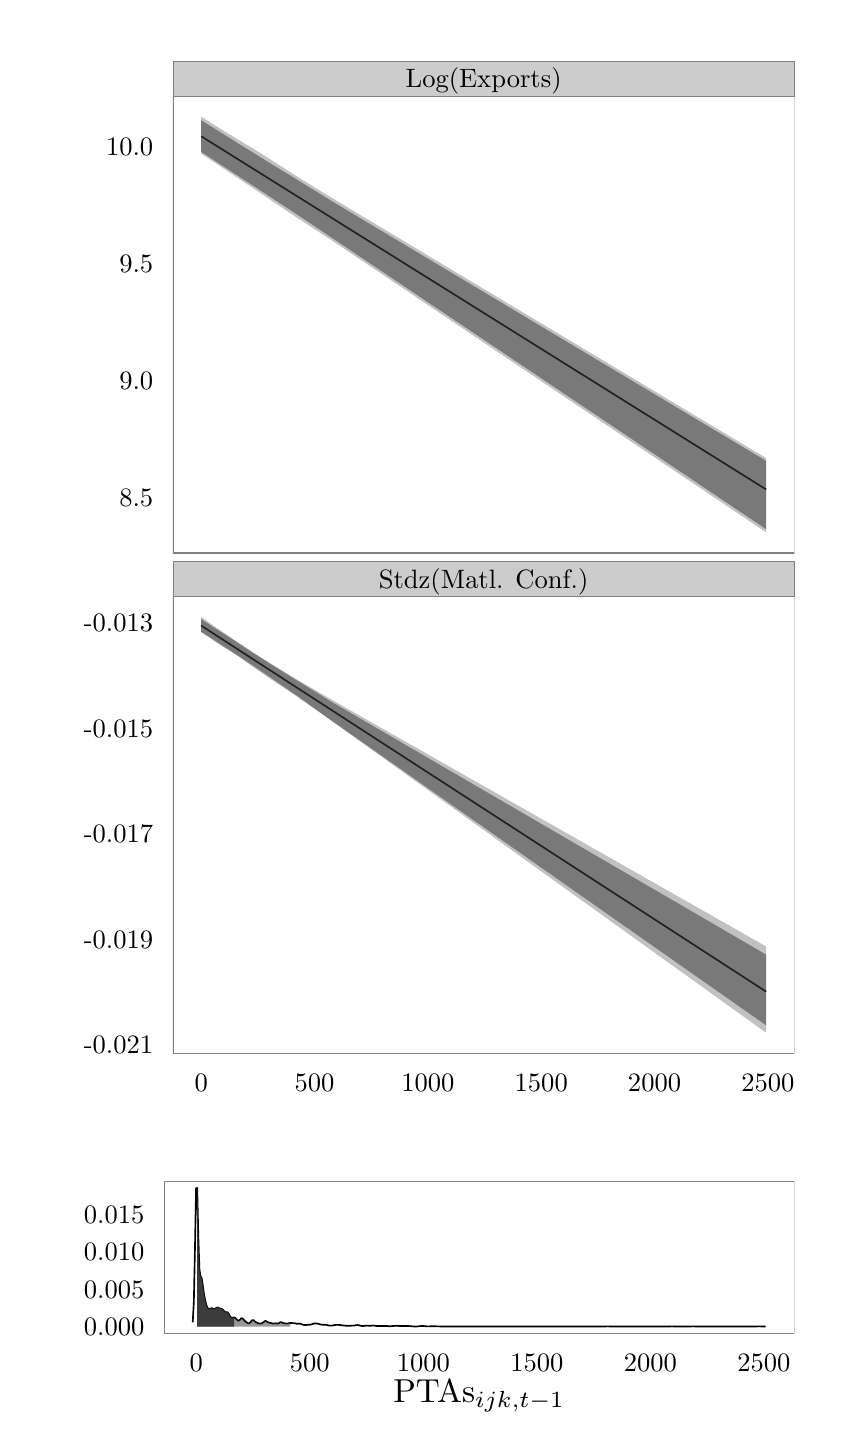
\begin{tikzpicture}[x=1pt,y=1pt]
\definecolor[named]{fillColor}{rgb}{1.00,1.00,1.00}
\path[use as bounding box,fill=fillColor,fill opacity=0.00] (0,0) rectangle (289.08,505.89);
\begin{scope}
\path[clip] (  0.00,101.18) rectangle (289.08,505.89);
\definecolor[named]{drawColor}{rgb}{1.00,1.00,1.00}
\definecolor[named]{fillColor}{rgb}{1.00,1.00,1.00}

\path[draw=drawColor,line width= 0.6pt,line join=round,line cap=round,fill=fillColor] (  0.00,101.18) rectangle (289.08,505.89);
\end{scope}
\begin{scope}
\path[clip] ( 52.48,316.03) rectangle (277.03,481.21);
\definecolor[named]{fillColor}{rgb}{1.00,1.00,1.00}

\path[fill=fillColor] ( 52.48,316.03) rectangle (277.03,481.21);
\definecolor[named]{drawColor}{rgb}{0.00,0.00,0.00}

\path[draw=drawColor,line width= 0.6pt,line join=round] ( 62.69,466.65) --
	( 62.94,466.50) --
	( 63.35,466.24) --
	( 64.08,465.78) --
	( 64.57,465.47) --
	( 65.31,465.01) --
	( 66.54,464.24) --
	( 68.26,463.17) --
	( 70.06,462.04) --
	( 71.70,461.02) --
	( 73.75,459.74) --
	( 76.53,458.00) --
	( 81.12,455.13) --
	( 88.08,450.77) --
	( 96.93,445.24) --
	(109.87,437.15) --
	(266.83,339.03);
\definecolor[named]{fillColor}{rgb}{0.20,0.20,0.20}

\path[fill=fillColor,fill opacity=0.30] ( 62.69,473.70) --
	( 62.94,473.55) --
	( 63.35,473.29) --
	( 64.08,472.84) --
	( 64.57,472.53) --
	( 65.31,472.07) --
	( 66.54,471.30) --
	( 68.26,470.23) --
	( 70.06,469.11) --
	( 71.70,468.09) --
	( 73.75,466.85) --
	( 76.53,465.17) --
	( 81.12,462.40) --
	( 88.08,458.06) --
	( 96.93,452.35) --
	(109.87,444.38) --
	(266.83,350.37) --
	(266.83,323.54) --
	(109.87,429.03) --
	( 96.93,437.47) --
	( 88.08,443.41) --
	( 81.12,448.09) --
	( 76.53,451.17) --
	( 73.75,453.04) --
	( 71.70,454.37) --
	( 70.06,455.47) --
	( 68.26,456.67) --
	( 66.54,457.82) --
	( 65.31,458.64) --
	( 64.57,459.13) --
	( 64.08,459.46) --
	( 63.35,459.95) --
	( 62.94,460.23) --
	( 62.69,460.39) --
	cycle;
\definecolor[named]{fillColor}{rgb}{0.20,0.20,0.20}

\path[fill=fillColor,fill opacity=0.50] ( 62.69,472.42) --
	( 62.94,472.27) --
	( 63.35,472.01) --
	( 64.08,471.55) --
	( 64.57,471.25) --
	( 65.31,470.79) --
	( 66.54,470.02) --
	( 68.26,468.95) --
	( 70.06,467.82) --
	( 71.70,466.80) --
	( 73.75,465.52) --
	( 76.53,463.78) --
	( 81.12,460.94) --
	( 88.08,456.62) --
	( 96.93,451.22) --
	(109.87,443.21) --
	(266.83,349.35) --
	(266.83,324.69) --
	(109.87,430.00) --
	( 96.93,438.67) --
	( 88.08,444.45) --
	( 81.12,449.01) --
	( 76.53,451.98) --
	( 73.75,453.80) --
	( 71.70,455.14) --
	( 70.06,456.20) --
	( 68.26,457.38) --
	( 66.54,458.50) --
	( 65.31,459.31) --
	( 64.57,459.80) --
	( 64.08,460.11) --
	( 63.35,460.58) --
	( 62.94,460.85) --
	( 62.69,461.01) --
	cycle;
\definecolor[named]{drawColor}{rgb}{0.50,0.50,0.50}

\path[draw=drawColor,line width= 0.6pt,line join=round,line cap=round] ( 52.48,316.03) rectangle (277.03,481.21);
\end{scope}
\begin{scope}
\path[clip] ( 52.48,135.21) rectangle (277.03,300.39);
\definecolor[named]{fillColor}{rgb}{1.00,1.00,1.00}

\path[fill=fillColor] ( 52.48,135.21) rectangle (277.03,300.39);
\definecolor[named]{drawColor}{rgb}{0.00,0.00,0.00}

\path[draw=drawColor,line width= 0.6pt,line join=round] ( 62.69,289.82) --
	( 62.94,289.67) --
	( 63.35,289.40) --
	( 64.08,288.92) --
	( 64.57,288.60) --
	( 65.31,288.13) --
	( 66.54,287.33) --
	( 68.26,286.22) --
	( 70.06,285.05) --
	( 71.70,283.99) --
	( 73.75,282.66) --
	( 76.53,280.86) --
	( 81.12,277.88) --
	( 88.08,273.37) --
	( 96.93,267.64) --
	(109.87,259.26) --
	(266.83,157.57);
\definecolor[named]{fillColor}{rgb}{0.20,0.20,0.20}

\path[fill=fillColor,fill opacity=0.30] ( 62.69,292.88) --
	( 62.94,292.73) --
	( 63.35,292.49) --
	( 64.08,291.99) --
	( 64.57,291.64) --
	( 65.31,291.11) --
	( 66.54,290.23) --
	( 68.26,289.02) --
	( 70.06,287.81) --
	( 71.70,286.70) --
	( 73.75,285.31) --
	( 76.53,283.42) --
	( 81.12,280.41) --
	( 88.08,275.97) --
	( 96.93,270.57) --
	(109.87,263.04) --
	(266.83,173.89) --
	(266.83,142.72) --
	(109.87,255.37) --
	( 96.93,264.45) --
	( 88.08,270.33) --
	( 81.12,275.14) --
	( 76.53,278.39) --
	( 73.75,280.32) --
	( 71.70,281.52) --
	( 70.06,282.45) --
	( 68.26,283.65) --
	( 66.54,284.82) --
	( 65.31,285.65) --
	( 64.57,286.15) --
	( 64.08,286.48) --
	( 63.35,286.97) --
	( 62.94,287.22) --
	( 62.69,287.36) --
	cycle;
\definecolor[named]{fillColor}{rgb}{0.20,0.20,0.20}

\path[fill=fillColor,fill opacity=0.50] ( 62.69,292.18) --
	( 62.94,292.01) --
	( 63.35,291.73) --
	( 64.08,291.25) --
	( 64.57,290.93) --
	( 65.31,290.45) --
	( 66.54,289.65) --
	( 68.26,288.54) --
	( 70.06,287.38) --
	( 71.70,286.32) --
	( 73.75,285.00) --
	( 76.53,283.19) --
	( 81.12,280.14) --
	( 88.08,275.72) --
	( 96.93,270.24) --
	(109.87,262.25) --
	(266.83,170.94) --
	(266.83,145.40) --
	(109.87,255.46) --
	( 96.93,264.75) --
	( 88.08,270.83) --
	( 81.12,275.56) --
	( 76.53,278.64) --
	( 73.75,280.40) --
	( 71.70,281.76) --
	( 70.06,282.86) --
	( 68.26,284.03) --
	( 66.54,285.14) --
	( 65.31,285.95) --
	( 64.57,286.41) --
	( 64.08,286.71) --
	( 63.35,287.18) --
	( 62.94,287.45) --
	( 62.69,287.61) --
	cycle;
\definecolor[named]{drawColor}{rgb}{0.50,0.50,0.50}

\path[draw=drawColor,line width= 0.6pt,line join=round,line cap=round] ( 52.48,135.21) rectangle (277.03,300.39);
\end{scope}
\begin{scope}
\path[clip] (  0.00,  0.00) rectangle (289.08,505.89);
\definecolor[named]{drawColor}{rgb}{0.50,0.50,0.50}
\definecolor[named]{fillColor}{rgb}{0.80,0.80,0.80}

\path[draw=drawColor,line width= 0.2pt,line join=round,line cap=round,fill=fillColor] ( 52.48,481.21) rectangle (277.03,493.84);
\definecolor[named]{drawColor}{rgb}{0.00,0.00,0.00}

\node[text=drawColor,anchor=base,inner sep=0pt, outer sep=0pt, scale=  0.96] at (164.76,484.22) {Log(Exports)};
\end{scope}
\begin{scope}
\path[clip] (  0.00,  0.00) rectangle (289.08,505.89);
\definecolor[named]{drawColor}{rgb}{0.50,0.50,0.50}
\definecolor[named]{fillColor}{rgb}{0.80,0.80,0.80}

\path[draw=drawColor,line width= 0.2pt,line join=round,line cap=round,fill=fillColor] ( 52.48,300.39) rectangle (277.03,313.02);
\definecolor[named]{drawColor}{rgb}{0.00,0.00,0.00}

\node[text=drawColor,anchor=base,inner sep=0pt, outer sep=0pt, scale=  0.96] at (164.76,303.40) {Stdz(Matl. Conf.)};
\end{scope}
\begin{scope}
\path[clip] (  0.00,  0.00) rectangle (289.08,505.89);
\definecolor[named]{drawColor}{rgb}{0.00,0.00,0.00}

\node[text=drawColor,anchor=base east,inner sep=0pt, outer sep=0pt, scale=  0.96] at ( 45.37,332.92) {8.5};

\node[text=drawColor,anchor=base east,inner sep=0pt, outer sep=0pt, scale=  0.96] at ( 45.37,375.13) {9.0};

\node[text=drawColor,anchor=base east,inner sep=0pt, outer sep=0pt, scale=  0.96] at ( 45.37,417.35) {9.5};

\node[text=drawColor,anchor=base east,inner sep=0pt, outer sep=0pt, scale=  0.96] at ( 45.37,459.56) {10.0};
\end{scope}
\begin{scope}
\path[clip] (  0.00,  0.00) rectangle (289.08,505.89);
\definecolor[named]{drawColor}{rgb}{0.00,0.00,0.00}

\node[text=drawColor,anchor=base east,inner sep=0pt, outer sep=0pt, scale=  0.96] at ( 45.37,135.03) {-0.021};

\node[text=drawColor,anchor=base east,inner sep=0pt, outer sep=0pt, scale=  0.96] at ( 45.37,173.19) {-0.019};

\node[text=drawColor,anchor=base east,inner sep=0pt, outer sep=0pt, scale=  0.96] at ( 45.37,211.34) {-0.017};

\node[text=drawColor,anchor=base east,inner sep=0pt, outer sep=0pt, scale=  0.96] at ( 45.37,249.50) {-0.015};

\node[text=drawColor,anchor=base east,inner sep=0pt, outer sep=0pt, scale=  0.96] at ( 45.37,287.65) {-0.013};
\end{scope}
\begin{scope}
\path[clip] (  0.00,  0.00) rectangle (289.08,505.89);
\definecolor[named]{drawColor}{rgb}{0.00,0.00,0.00}

\node[text=drawColor,anchor=base,inner sep=0pt, outer sep=0pt, scale=  0.96] at ( 62.69,121.49) {0};

\node[text=drawColor,anchor=base,inner sep=0pt, outer sep=0pt, scale=  0.96] at (103.65,121.49) {500};

\node[text=drawColor,anchor=base,inner sep=0pt, outer sep=0pt, scale=  0.96] at (144.61,121.49) {1000};

\node[text=drawColor,anchor=base,inner sep=0pt, outer sep=0pt, scale=  0.96] at (185.57,121.49) {1500};

\node[text=drawColor,anchor=base,inner sep=0pt, outer sep=0pt, scale=  0.96] at (226.52,121.49) {2000};

\node[text=drawColor,anchor=base,inner sep=0pt, outer sep=0pt, scale=  0.96] at (267.48,121.49) {2500};
\end{scope}
\begin{scope}
\path[clip] (  0.00,  0.00) rectangle (289.08,101.18);
\definecolor[named]{drawColor}{rgb}{1.00,1.00,1.00}
\definecolor[named]{fillColor}{rgb}{1.00,1.00,1.00}

\path[draw=drawColor,line width= 0.6pt,line join=round,line cap=round,fill=fillColor] ( -0.00,  0.00) rectangle (289.08,101.18);
\end{scope}
\begin{scope}
\path[clip] ( 49.28, 34.03) rectangle (277.04, 89.13);
\definecolor[named]{fillColor}{rgb}{1.00,1.00,1.00}

\path[fill=fillColor] ( 49.28, 34.03) rectangle (277.04, 89.13);
\definecolor[named]{drawColor}{rgb}{0.00,0.00,0.00}

\path[draw=drawColor,line width= 0.6pt,line join=round] ( 59.64, 38.05) --
	( 60.04, 45.39) --
	( 60.45, 64.85) --
	( 60.85, 86.49) --
	( 61.26, 86.63) --
	( 61.66, 69.17) --
	( 62.07, 57.11) --
	( 62.47, 54.76) --
	( 62.88, 53.97) --
	( 63.28, 51.42) --
	( 63.69, 48.50) --
	( 64.09, 46.23) --
	( 64.50, 44.54) --
	( 64.90, 43.44) --
	( 65.31, 43.00) --
	( 65.71, 42.85) --
	( 66.12, 43.03) --
	( 66.52, 43.25) --
	( 66.93, 42.98) --
	( 67.33, 42.78) --
	( 67.74, 42.97) --
	( 68.15, 43.27) --
	( 68.55, 43.45) --
	( 68.96, 43.34) --
	( 69.36, 43.10) --
	( 69.77, 42.99) --
	( 70.17, 42.90) --
	( 70.58, 42.58) --
	( 70.98, 42.09) --
	( 71.39, 41.76) --
	( 71.79, 41.75) --
	( 72.20, 41.71) --
	( 72.60, 41.19) --
	( 73.01, 40.38) --
	( 73.41, 39.86) --
	( 73.82, 39.74) --
	( 74.22, 39.79) --
	( 74.63, 39.79) --
	( 75.03, 39.62) --
	( 75.44, 39.22) --
	( 75.84, 38.78) --
	( 76.25, 38.63) --
	( 76.65, 38.91) --
	( 77.06, 39.40) --
	( 77.46, 39.57) --
	( 77.87, 39.24) --
	( 78.27, 38.74) --
	( 78.68, 38.34) --
	( 79.09, 38.05) --
	( 79.49, 37.81) --
	( 79.90, 37.72) --
	( 80.30, 37.87) --
	( 80.71, 38.33) --
	( 81.11, 38.84) --
	( 81.52, 38.88) --
	( 81.92, 38.51) --
	( 82.33, 38.20) --
	( 82.73, 37.99) --
	( 83.14, 37.79) --
	( 83.54, 37.66) --
	( 83.95, 37.62) --
	( 84.35, 37.65) --
	( 84.76, 37.79) --
	( 85.16, 38.04) --
	( 85.57, 38.41) --
	( 85.97, 38.60) --
	( 86.38, 38.39) --
	( 86.78, 38.11) --
	( 87.19, 37.98) --
	( 87.59, 37.88) --
	( 88.00, 37.77) --
	( 88.40, 37.67) --
	( 88.81, 37.64) --
	( 89.21, 37.69) --
	( 89.62, 37.71) --
	( 90.02, 37.64) --
	( 90.43, 37.64) --
	( 90.84, 37.81) --
	( 91.24, 38.06) --
	( 91.65, 38.11) --
	( 92.05, 37.92) --
	( 92.46, 37.76) --
	( 92.86, 37.72) --
	( 93.27, 37.65) --
	( 93.67, 37.58) --
	( 94.08, 37.64) --
	( 94.48, 37.78) --
	( 94.89, 37.84) --
	( 95.29, 37.80) --
	( 95.70, 37.78) --
	( 96.10, 37.79) --
	( 96.51, 37.75) --
	( 96.91, 37.64) --
	( 97.32, 37.53) --
	( 97.72, 37.54) --
	( 98.13, 37.61) --
	( 98.53, 37.56) --
	( 98.94, 37.39) --
	( 99.34, 37.23) --
	( 99.75, 37.13) --
	(100.15, 37.11) --
	(100.56, 37.11) --
	(100.96, 37.14) --
	(101.37, 37.17) --
	(101.78, 37.19) --
	(102.18, 37.23) --
	(102.59, 37.33) --
	(102.99, 37.49) --
	(103.40, 37.62) --
	(103.80, 37.65) --
	(104.21, 37.62) --
	(104.61, 37.61) --
	(105.02, 37.53) --
	(105.42, 37.39) --
	(105.83, 37.28) --
	(106.23, 37.23) --
	(106.64, 37.20) --
	(107.04, 37.20) --
	(107.45, 37.21) --
	(107.85, 37.16) --
	(108.26, 37.05) --
	(108.66, 36.93) --
	(109.07, 36.88) --
	(109.47, 36.87) --
	(109.88, 36.89) --
	(110.28, 36.96) --
	(110.69, 37.05) --
	(111.09, 37.11) --
	(111.50, 37.13) --
	(111.90, 37.13) --
	(112.31, 37.13) --
	(112.71, 37.12) --
	(113.12, 37.08) --
	(113.53, 36.99) --
	(113.93, 36.93) --
	(114.34, 36.91) --
	(114.74, 36.86) --
	(115.15, 36.82) --
	(115.55, 36.82) --
	(115.96, 36.85) --
	(116.36, 36.85) --
	(116.77, 36.85) --
	(117.17, 36.86) --
	(117.58, 36.88) --
	(117.98, 36.91) --
	(118.39, 36.99) --
	(118.79, 37.06) --
	(119.20, 37.08) --
	(119.60, 37.03) --
	(120.01, 36.93) --
	(120.41, 36.82) --
	(120.82, 36.75) --
	(121.22, 36.75) --
	(121.63, 36.79) --
	(122.03, 36.84) --
	(122.44, 36.86) --
	(122.84, 36.87) --
	(123.25, 36.85) --
	(123.65, 36.82) --
	(124.06, 36.83) --
	(124.47, 36.88) --
	(124.87, 36.90) --
	(125.28, 36.87) --
	(125.68, 36.80) --
	(126.09, 36.74) --
	(126.49, 36.72) --
	(126.90, 36.72) --
	(127.30, 36.71) --
	(127.71, 36.71) --
	(128.11, 36.72) --
	(128.52, 36.74) --
	(128.92, 36.76) --
	(129.33, 36.76) --
	(129.73, 36.75) --
	(130.14, 36.71) --
	(130.54, 36.67) --
	(130.95, 36.65) --
	(131.35, 36.68) --
	(131.76, 36.73) --
	(132.16, 36.76) --
	(132.57, 36.77) --
	(132.97, 36.80) --
	(133.38, 36.81) --
	(133.78, 36.78) --
	(134.19, 36.76) --
	(134.59, 36.74) --
	(135.00, 36.73) --
	(135.40, 36.73) --
	(135.81, 36.73) --
	(136.22, 36.72) --
	(136.62, 36.73) --
	(137.03, 36.75) --
	(137.43, 36.73) --
	(137.84, 36.71) --
	(138.24, 36.69) --
	(138.65, 36.64) --
	(139.05, 36.60) --
	(139.46, 36.58) --
	(139.86, 36.57) --
	(140.27, 36.57) --
	(140.67, 36.59) --
	(141.08, 36.61) --
	(141.48, 36.65) --
	(141.89, 36.71) --
	(142.29, 36.74) --
	(142.70, 36.73) --
	(143.10, 36.72) --
	(143.51, 36.69) --
	(143.91, 36.64) --
	(144.32, 36.60) --
	(144.72, 36.60) --
	(145.13, 36.61) --
	(145.53, 36.63) --
	(145.94, 36.64) --
	(146.34, 36.64) --
	(146.75, 36.64) --
	(147.16, 36.64) --
	(147.56, 36.62) --
	(147.97, 36.61) --
	(148.37, 36.60) --
	(148.78, 36.59) --
	(149.18, 36.57) --
	(149.59, 36.57) --
	(149.99, 36.57) --
	(150.40, 36.58) --
	(150.80, 36.58) --
	(151.21, 36.57) --
	(151.61, 36.57) --
	(152.02, 36.57) --
	(152.42, 36.56) --
	(152.83, 36.55) --
	(153.23, 36.54) --
	(153.64, 36.54) --
	(154.04, 36.54) --
	(154.45, 36.54) --
	(154.85, 36.54) --
	(155.26, 36.54) --
	(155.66, 36.54) --
	(156.07, 36.54) --
	(156.47, 36.54) --
	(156.88, 36.54) --
	(157.28, 36.54) --
	(157.69, 36.54) --
	(158.09, 36.54) --
	(158.50, 36.54) --
	(158.91, 36.54) --
	(159.31, 36.54) --
	(159.72, 36.54) --
	(160.12, 36.54) --
	(160.53, 36.54) --
	(160.93, 36.54) --
	(161.34, 36.54) --
	(161.74, 36.54) --
	(162.15, 36.55) --
	(162.55, 36.56) --
	(162.96, 36.56) --
	(163.36, 36.57) --
	(163.77, 36.56) --
	(164.17, 36.56) --
	(164.58, 36.55) --
	(164.98, 36.55) --
	(165.39, 36.54) --
	(165.79, 36.54) --
	(166.20, 36.55) --
	(166.60, 36.56) --
	(167.01, 36.58) --
	(167.41, 36.58) --
	(167.82, 36.58) --
	(168.22, 36.57) --
	(168.63, 36.56) --
	(169.03, 36.56) --
	(169.44, 36.55) --
	(169.85, 36.55) --
	(170.25, 36.55) --
	(170.66, 36.55) --
	(171.06, 36.55) --
	(171.47, 36.55) --
	(171.87, 36.55) --
	(172.28, 36.54) --
	(172.68, 36.54) --
	(173.09, 36.54) --
	(173.49, 36.54) --
	(173.90, 36.54) --
	(174.30, 36.54) --
	(174.71, 36.54) --
	(175.11, 36.54) --
	(175.52, 36.54) --
	(175.92, 36.54) --
	(176.33, 36.54) --
	(176.73, 36.54) --
	(177.14, 36.54) --
	(177.54, 36.54) --
	(177.95, 36.54) --
	(178.35, 36.54) --
	(178.76, 36.54) --
	(179.16, 36.54) --
	(179.57, 36.54) --
	(179.97, 36.54) --
	(180.38, 36.54) --
	(180.78, 36.54) --
	(181.19, 36.54) --
	(181.60, 36.54) --
	(182.00, 36.54) --
	(182.41, 36.54) --
	(182.81, 36.54) --
	(183.22, 36.54) --
	(183.62, 36.54) --
	(184.03, 36.54) --
	(184.43, 36.54) --
	(184.84, 36.54) --
	(185.24, 36.55) --
	(185.65, 36.55) --
	(186.05, 36.55) --
	(186.46, 36.54) --
	(186.86, 36.54) --
	(187.27, 36.54) --
	(187.67, 36.55) --
	(188.08, 36.55) --
	(188.48, 36.55) --
	(188.89, 36.56) --
	(189.29, 36.56) --
	(189.70, 36.56) --
	(190.10, 36.56) --
	(190.51, 36.55) --
	(190.91, 36.55) --
	(191.32, 36.54) --
	(191.72, 36.54) --
	(192.13, 36.54) --
	(192.54, 36.54) --
	(192.94, 36.54) --
	(193.35, 36.54) --
	(193.75, 36.54) --
	(194.16, 36.54) --
	(194.56, 36.54) --
	(194.97, 36.54) --
	(195.37, 36.54) --
	(195.78, 36.54) --
	(196.18, 36.54) --
	(196.59, 36.54) --
	(196.99, 36.54) --
	(197.40, 36.54) --
	(197.80, 36.54) --
	(198.21, 36.54) --
	(198.61, 36.54) --
	(199.02, 36.54) --
	(199.42, 36.54) --
	(199.83, 36.54) --
	(200.23, 36.54) --
	(200.64, 36.54) --
	(201.04, 36.54) --
	(201.45, 36.54) --
	(201.85, 36.54) --
	(202.26, 36.54) --
	(202.66, 36.54) --
	(203.07, 36.54) --
	(203.47, 36.54) --
	(203.88, 36.54) --
	(204.29, 36.54) --
	(204.69, 36.54) --
	(205.10, 36.54) --
	(205.50, 36.54) --
	(205.91, 36.54) --
	(206.31, 36.55) --
	(206.72, 36.56) --
	(207.12, 36.57) --
	(207.53, 36.58) --
	(207.93, 36.57) --
	(208.34, 36.57) --
	(208.74, 36.57) --
	(209.15, 36.59) --
	(209.55, 36.60) --
	(209.96, 36.59) --
	(210.36, 36.57) --
	(210.77, 36.55) --
	(211.17, 36.54) --
	(211.58, 36.54) --
	(211.98, 36.54) --
	(212.39, 36.54) --
	(212.79, 36.54) --
	(213.20, 36.54) --
	(213.60, 36.54) --
	(214.01, 36.54) --
	(214.41, 36.54) --
	(214.82, 36.54) --
	(215.23, 36.54) --
	(215.63, 36.54) --
	(216.04, 36.54) --
	(216.44, 36.54) --
	(216.85, 36.54) --
	(217.25, 36.54) --
	(217.66, 36.54) --
	(218.06, 36.54) --
	(218.47, 36.54) --
	(218.87, 36.54) --
	(219.28, 36.54) --
	(219.68, 36.54) --
	(220.09, 36.54) --
	(220.49, 36.54) --
	(220.90, 36.54) --
	(221.30, 36.54) --
	(221.71, 36.54) --
	(222.11, 36.54) --
	(222.52, 36.54) --
	(222.92, 36.54) --
	(223.33, 36.54) --
	(223.73, 36.54) --
	(224.14, 36.54) --
	(224.54, 36.55) --
	(224.95, 36.55) --
	(225.35, 36.55) --
	(225.76, 36.54) --
	(226.16, 36.54) --
	(226.57, 36.54) --
	(226.98, 36.54) --
	(227.38, 36.54) --
	(227.79, 36.54) --
	(228.19, 36.54) --
	(228.60, 36.54) --
	(229.00, 36.54) --
	(229.41, 36.55) --
	(229.81, 36.56) --
	(230.22, 36.57) --
	(230.62, 36.57) --
	(231.03, 36.56) --
	(231.43, 36.56) --
	(231.84, 36.57) --
	(232.24, 36.58) --
	(232.65, 36.59) --
	(233.05, 36.59) --
	(233.46, 36.58) --
	(233.86, 36.56) --
	(234.27, 36.55) --
	(234.67, 36.54) --
	(235.08, 36.54) --
	(235.48, 36.54) --
	(235.89, 36.54) --
	(236.29, 36.54) --
	(236.70, 36.54) --
	(237.10, 36.54) --
	(237.51, 36.54) --
	(237.92, 36.54) --
	(238.32, 36.54) --
	(238.73, 36.55) --
	(239.13, 36.56) --
	(239.54, 36.57) --
	(239.94, 36.59) --
	(240.35, 36.61) --
	(240.75, 36.60) --
	(241.16, 36.57) --
	(241.56, 36.55) --
	(241.97, 36.54) --
	(242.37, 36.54) --
	(242.78, 36.54) --
	(243.18, 36.54) --
	(243.59, 36.54) --
	(243.99, 36.54) --
	(244.40, 36.54) --
	(244.80, 36.54) --
	(245.21, 36.54) --
	(245.61, 36.54) --
	(246.02, 36.54) --
	(246.42, 36.54) --
	(246.83, 36.54) --
	(247.23, 36.54) --
	(247.64, 36.54) --
	(248.04, 36.54) --
	(248.45, 36.54) --
	(248.85, 36.54) --
	(249.26, 36.54) --
	(249.67, 36.54) --
	(250.07, 36.54) --
	(250.48, 36.54) --
	(250.88, 36.54) --
	(251.29, 36.54) --
	(251.69, 36.54) --
	(252.10, 36.54) --
	(252.50, 36.54) --
	(252.91, 36.54) --
	(253.31, 36.54) --
	(253.72, 36.54) --
	(254.12, 36.54) --
	(254.53, 36.54) --
	(254.93, 36.54) --
	(255.34, 36.54) --
	(255.74, 36.55) --
	(256.15, 36.55) --
	(256.55, 36.55) --
	(256.96, 36.55) --
	(257.36, 36.54) --
	(257.77, 36.54) --
	(258.17, 36.54) --
	(258.58, 36.54) --
	(258.98, 36.54) --
	(259.39, 36.54) --
	(259.79, 36.54) --
	(260.20, 36.54) --
	(260.61, 36.54) --
	(261.01, 36.54) --
	(261.42, 36.54) --
	(261.82, 36.54) --
	(262.23, 36.54) --
	(262.63, 36.55) --
	(263.04, 36.56) --
	(263.44, 36.57) --
	(263.85, 36.60) --
	(264.25, 36.61) --
	(264.66, 36.60) --
	(265.06, 36.58) --
	(265.47, 36.56) --
	(265.87, 36.55) --
	(266.28, 36.54) --
	(266.68, 36.54);
\definecolor[named]{fillColor}{rgb}{0.20,0.20,0.20}

\path[fill=fillColor,fill opacity=0.50] ( 61.26, 86.63) --
	( 61.66, 69.17) --
	( 62.07, 57.11) --
	( 62.47, 54.76) --
	( 62.88, 53.97) --
	( 63.28, 51.42) --
	( 63.69, 48.50) --
	( 64.09, 46.23) --
	( 64.50, 44.54) --
	( 64.90, 43.44) --
	( 65.31, 43.00) --
	( 65.71, 42.85) --
	( 66.12, 43.03) --
	( 66.52, 43.25) --
	( 66.93, 42.98) --
	( 67.33, 42.78) --
	( 67.74, 42.97) --
	( 68.15, 43.27) --
	( 68.55, 43.45) --
	( 68.96, 43.34) --
	( 69.36, 43.10) --
	( 69.77, 42.99) --
	( 70.17, 42.90) --
	( 70.58, 42.58) --
	( 70.98, 42.09) --
	( 71.39, 41.76) --
	( 71.79, 41.75) --
	( 72.20, 41.71) --
	( 72.60, 41.19) --
	( 73.01, 40.38) --
	( 73.41, 39.86) --
	( 73.82, 39.74) --
	( 74.22, 39.79) --
	( 74.63, 39.79) --
	( 75.03, 39.62) --
	( 75.44, 39.22) --
	( 75.84, 38.78) --
	( 76.25, 38.63) --
	( 76.65, 38.91) --
	( 77.06, 39.40) --
	( 77.46, 39.57) --
	( 77.87, 39.24) --
	( 78.27, 38.74) --
	( 78.68, 38.34) --
	( 79.09, 38.05) --
	( 79.49, 37.81) --
	( 79.90, 37.72) --
	( 80.30, 37.87) --
	( 80.71, 38.33) --
	( 81.11, 38.84) --
	( 81.52, 38.88) --
	( 81.92, 38.51) --
	( 82.33, 38.20) --
	( 82.73, 37.99) --
	( 83.14, 37.79) --
	( 83.54, 37.66) --
	( 83.95, 37.62) --
	( 84.35, 37.65) --
	( 84.76, 37.79) --
	( 85.16, 38.04) --
	( 85.57, 38.41) --
	( 85.97, 38.60) --
	( 86.38, 38.39) --
	( 86.78, 38.11) --
	( 87.19, 37.98) --
	( 87.59, 37.88) --
	( 88.00, 37.77) --
	( 88.40, 37.67) --
	( 88.81, 37.64) --
	( 89.21, 37.69) --
	( 89.62, 37.71) --
	( 90.02, 37.64) --
	( 90.43, 37.64) --
	( 90.84, 37.81) --
	( 91.24, 38.06) --
	( 91.65, 38.11) --
	( 92.05, 37.92) --
	( 92.46, 37.76) --
	( 92.86, 37.72) --
	( 93.27, 37.65) --
	( 93.67, 37.58) --
	( 94.08, 37.64) --
	( 94.48, 37.78) --
	( 94.89, 37.84) --
	( 94.89, 36.54) --
	( 94.48, 36.54) --
	( 94.08, 36.54) --
	( 93.67, 36.54) --
	( 93.27, 36.54) --
	( 92.86, 36.54) --
	( 92.46, 36.54) --
	( 92.05, 36.54) --
	( 91.65, 36.54) --
	( 91.24, 36.54) --
	( 90.84, 36.54) --
	( 90.43, 36.54) --
	( 90.02, 36.54) --
	( 89.62, 36.54) --
	( 89.21, 36.54) --
	( 88.81, 36.54) --
	( 88.40, 36.54) --
	( 88.00, 36.54) --
	( 87.59, 36.54) --
	( 87.19, 36.54) --
	( 86.78, 36.54) --
	( 86.38, 36.54) --
	( 85.97, 36.54) --
	( 85.57, 36.54) --
	( 85.16, 36.54) --
	( 84.76, 36.54) --
	( 84.35, 36.54) --
	( 83.95, 36.54) --
	( 83.54, 36.54) --
	( 83.14, 36.54) --
	( 82.73, 36.54) --
	( 82.33, 36.54) --
	( 81.92, 36.54) --
	( 81.52, 36.54) --
	( 81.11, 36.54) --
	( 80.71, 36.54) --
	( 80.30, 36.54) --
	( 79.90, 36.54) --
	( 79.49, 36.54) --
	( 79.09, 36.54) --
	( 78.68, 36.54) --
	( 78.27, 36.54) --
	( 77.87, 36.54) --
	( 77.46, 36.54) --
	( 77.06, 36.54) --
	( 76.65, 36.54) --
	( 76.25, 36.54) --
	( 75.84, 36.54) --
	( 75.44, 36.54) --
	( 75.03, 36.54) --
	( 74.63, 36.54) --
	( 74.22, 36.54) --
	( 73.82, 36.54) --
	( 73.41, 36.54) --
	( 73.01, 36.54) --
	( 72.60, 36.54) --
	( 72.20, 36.54) --
	( 71.79, 36.54) --
	( 71.39, 36.54) --
	( 70.98, 36.54) --
	( 70.58, 36.54) --
	( 70.17, 36.54) --
	( 69.77, 36.54) --
	( 69.36, 36.54) --
	( 68.96, 36.54) --
	( 68.55, 36.54) --
	( 68.15, 36.54) --
	( 67.74, 36.54) --
	( 67.33, 36.54) --
	( 66.93, 36.54) --
	( 66.52, 36.54) --
	( 66.12, 36.54) --
	( 65.71, 36.54) --
	( 65.31, 36.54) --
	( 64.90, 36.54) --
	( 64.50, 36.54) --
	( 64.09, 36.54) --
	( 63.69, 36.54) --
	( 63.28, 36.54) --
	( 62.88, 36.54) --
	( 62.47, 36.54) --
	( 62.07, 36.54) --
	( 61.66, 36.54) --
	( 61.26, 36.54) --
	cycle;
\definecolor[named]{fillColor}{rgb}{0.20,0.20,0.20}

\path[fill=fillColor,fill opacity=0.90] ( 61.26, 86.63) --
	( 61.66, 69.17) --
	( 62.07, 57.11) --
	( 62.47, 54.76) --
	( 62.88, 53.97) --
	( 63.28, 51.42) --
	( 63.69, 48.50) --
	( 64.09, 46.23) --
	( 64.50, 44.54) --
	( 64.90, 43.44) --
	( 65.31, 43.00) --
	( 65.71, 42.85) --
	( 66.12, 43.03) --
	( 66.52, 43.25) --
	( 66.93, 42.98) --
	( 67.33, 42.78) --
	( 67.74, 42.97) --
	( 68.15, 43.27) --
	( 68.55, 43.45) --
	( 68.96, 43.34) --
	( 69.36, 43.10) --
	( 69.77, 42.99) --
	( 70.17, 42.90) --
	( 70.58, 42.58) --
	( 70.98, 42.09) --
	( 71.39, 41.76) --
	( 71.79, 41.75) --
	( 72.20, 41.71) --
	( 72.60, 41.19) --
	( 73.01, 40.38) --
	( 73.41, 39.86) --
	( 73.82, 39.74) --
	( 74.22, 39.79) --
	( 74.63, 39.79) --
	( 74.63, 36.54) --
	( 74.22, 36.54) --
	( 73.82, 36.54) --
	( 73.41, 36.54) --
	( 73.01, 36.54) --
	( 72.60, 36.54) --
	( 72.20, 36.54) --
	( 71.79, 36.54) --
	( 71.39, 36.54) --
	( 70.98, 36.54) --
	( 70.58, 36.54) --
	( 70.17, 36.54) --
	( 69.77, 36.54) --
	( 69.36, 36.54) --
	( 68.96, 36.54) --
	( 68.55, 36.54) --
	( 68.15, 36.54) --
	( 67.74, 36.54) --
	( 67.33, 36.54) --
	( 66.93, 36.54) --
	( 66.52, 36.54) --
	( 66.12, 36.54) --
	( 65.71, 36.54) --
	( 65.31, 36.54) --
	( 64.90, 36.54) --
	( 64.50, 36.54) --
	( 64.09, 36.54) --
	( 63.69, 36.54) --
	( 63.28, 36.54) --
	( 62.88, 36.54) --
	( 62.47, 36.54) --
	( 62.07, 36.54) --
	( 61.66, 36.54) --
	( 61.26, 36.54) --
	cycle;
\definecolor[named]{drawColor}{rgb}{0.50,0.50,0.50}

\path[draw=drawColor,line width= 0.6pt,line join=round,line cap=round] ( 49.28, 34.03) rectangle (277.04, 89.13);
\end{scope}
\begin{scope}
\path[clip] (  0.00,  0.00) rectangle (289.08,505.89);
\definecolor[named]{drawColor}{rgb}{0.00,0.00,0.00}

\node[text=drawColor,anchor=base east,inner sep=0pt, outer sep=0pt, scale=  0.96] at ( 42.17, 33.23) {0.000};

\node[text=drawColor,anchor=base east,inner sep=0pt, outer sep=0pt, scale=  0.96] at ( 42.17, 46.79) {0.005};

\node[text=drawColor,anchor=base east,inner sep=0pt, outer sep=0pt, scale=  0.96] at ( 42.17, 60.35) {0.010};

\node[text=drawColor,anchor=base east,inner sep=0pt, outer sep=0pt, scale=  0.96] at ( 42.17, 73.92) {0.015};
\end{scope}
\begin{scope}
\path[clip] (  0.00,  0.00) rectangle (289.08,505.89);
\definecolor[named]{drawColor}{rgb}{0.00,0.00,0.00}

\node[text=drawColor,anchor=base,inner sep=0pt, outer sep=0pt, scale=  0.96] at ( 60.93, 20.31) {0};

\node[text=drawColor,anchor=base,inner sep=0pt, outer sep=0pt, scale=  0.96] at (101.95, 20.31) {500};

\node[text=drawColor,anchor=base,inner sep=0pt, outer sep=0pt, scale=  0.96] at (142.98, 20.31) {1000};

\node[text=drawColor,anchor=base,inner sep=0pt, outer sep=0pt, scale=  0.96] at (184.00, 20.31) {1500};

\node[text=drawColor,anchor=base,inner sep=0pt, outer sep=0pt, scale=  0.96] at (225.02, 20.31) {2000};

\node[text=drawColor,anchor=base,inner sep=0pt, outer sep=0pt, scale=  0.96] at (266.04, 20.31) {2500};
\end{scope}
\begin{scope}
\path[clip] (  0.00,  0.00) rectangle (289.08,505.89);
\definecolor[named]{drawColor}{rgb}{0.00,0.00,0.00}

\node[text=drawColor,anchor=base,inner sep=0pt, outer sep=0pt, scale=  1.20] at (163.16,  9.03) {PTAs$_{ijk, t-1}$};
\end{scope}
\end{tikzpicture}
}  &
      \resizebox{.45\textwidth}{!}{% Created by tikzDevice version 0.7.0 on 2015-07-01 08:58:18
% !TEX encoding = UTF-8 Unicode
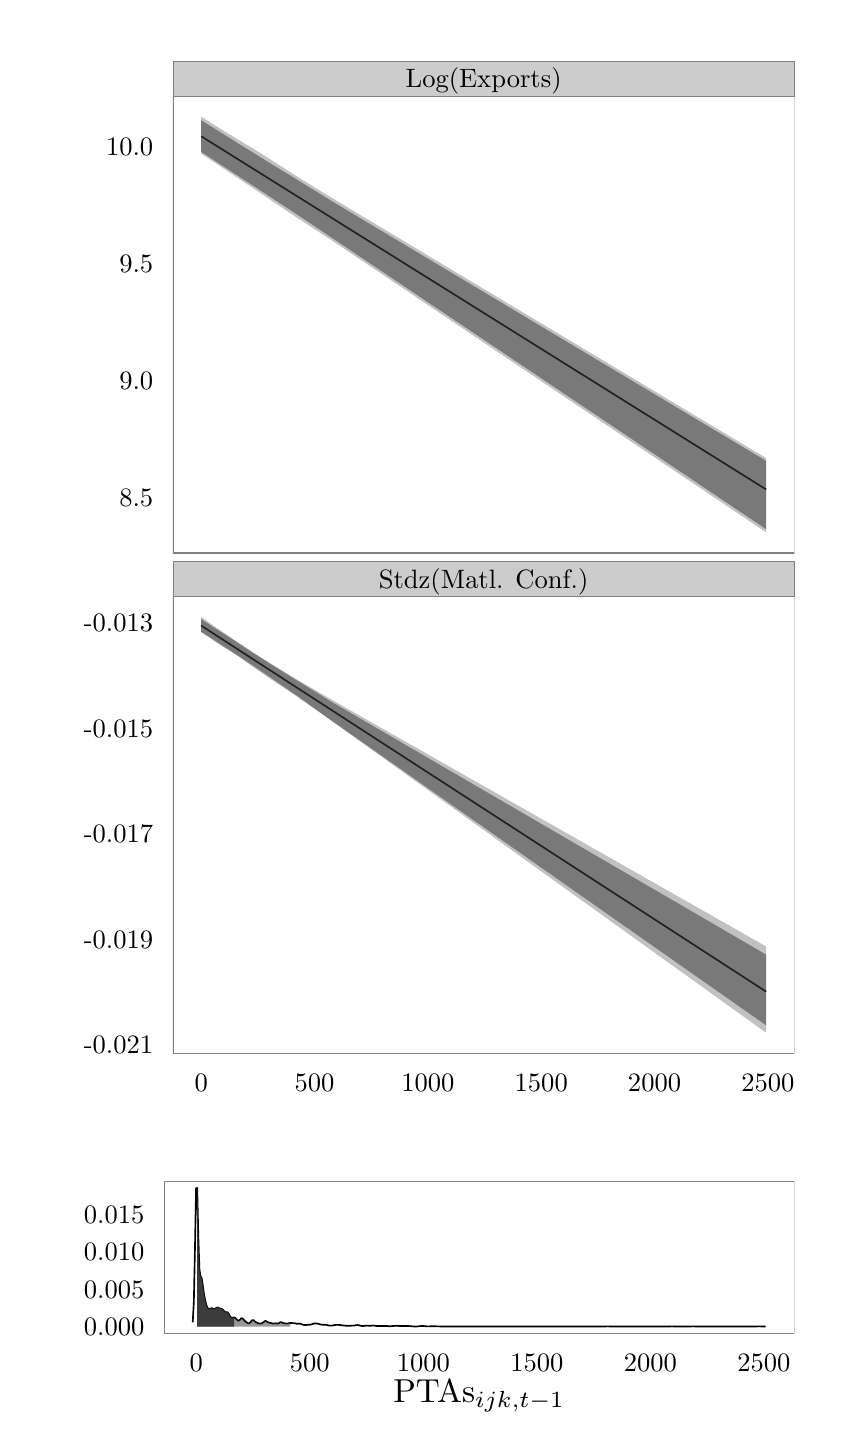
\begin{tikzpicture}[x=1pt,y=1pt]
\definecolor[named]{fillColor}{rgb}{1.00,1.00,1.00}
\path[use as bounding box,fill=fillColor,fill opacity=0.00] (0,0) rectangle (289.08,505.89);
\begin{scope}
\path[clip] (  0.00,101.18) rectangle (289.08,505.89);
\definecolor[named]{drawColor}{rgb}{1.00,1.00,1.00}
\definecolor[named]{fillColor}{rgb}{1.00,1.00,1.00}

\path[draw=drawColor,line width= 0.6pt,line join=round,line cap=round,fill=fillColor] (  0.00,101.18) rectangle (289.08,505.89);
\end{scope}
\begin{scope}
\path[clip] ( 52.48,316.03) rectangle (277.03,481.21);
\definecolor[named]{fillColor}{rgb}{1.00,1.00,1.00}

\path[fill=fillColor] ( 52.48,316.03) rectangle (277.03,481.21);
\definecolor[named]{drawColor}{rgb}{0.00,0.00,0.00}

\path[draw=drawColor,line width= 0.6pt,line join=round] ( 62.69,466.65) --
	( 62.94,466.50) --
	( 63.35,466.24) --
	( 64.08,465.78) --
	( 64.57,465.47) --
	( 65.31,465.01) --
	( 66.54,464.24) --
	( 68.26,463.17) --
	( 70.06,462.04) --
	( 71.70,461.02) --
	( 73.75,459.74) --
	( 76.53,458.00) --
	( 81.12,455.13) --
	( 88.08,450.77) --
	( 96.93,445.24) --
	(109.87,437.15) --
	(266.83,339.03);
\definecolor[named]{fillColor}{rgb}{0.20,0.20,0.20}

\path[fill=fillColor,fill opacity=0.30] ( 62.69,473.70) --
	( 62.94,473.55) --
	( 63.35,473.29) --
	( 64.08,472.84) --
	( 64.57,472.53) --
	( 65.31,472.07) --
	( 66.54,471.30) --
	( 68.26,470.23) --
	( 70.06,469.11) --
	( 71.70,468.09) --
	( 73.75,466.85) --
	( 76.53,465.17) --
	( 81.12,462.40) --
	( 88.08,458.06) --
	( 96.93,452.35) --
	(109.87,444.38) --
	(266.83,350.37) --
	(266.83,323.54) --
	(109.87,429.03) --
	( 96.93,437.47) --
	( 88.08,443.41) --
	( 81.12,448.09) --
	( 76.53,451.17) --
	( 73.75,453.04) --
	( 71.70,454.37) --
	( 70.06,455.47) --
	( 68.26,456.67) --
	( 66.54,457.82) --
	( 65.31,458.64) --
	( 64.57,459.13) --
	( 64.08,459.46) --
	( 63.35,459.95) --
	( 62.94,460.23) --
	( 62.69,460.39) --
	cycle;
\definecolor[named]{fillColor}{rgb}{0.20,0.20,0.20}

\path[fill=fillColor,fill opacity=0.50] ( 62.69,472.42) --
	( 62.94,472.27) --
	( 63.35,472.01) --
	( 64.08,471.55) --
	( 64.57,471.25) --
	( 65.31,470.79) --
	( 66.54,470.02) --
	( 68.26,468.95) --
	( 70.06,467.82) --
	( 71.70,466.80) --
	( 73.75,465.52) --
	( 76.53,463.78) --
	( 81.12,460.94) --
	( 88.08,456.62) --
	( 96.93,451.22) --
	(109.87,443.21) --
	(266.83,349.35) --
	(266.83,324.69) --
	(109.87,430.00) --
	( 96.93,438.67) --
	( 88.08,444.45) --
	( 81.12,449.01) --
	( 76.53,451.98) --
	( 73.75,453.80) --
	( 71.70,455.14) --
	( 70.06,456.20) --
	( 68.26,457.38) --
	( 66.54,458.50) --
	( 65.31,459.31) --
	( 64.57,459.80) --
	( 64.08,460.11) --
	( 63.35,460.58) --
	( 62.94,460.85) --
	( 62.69,461.01) --
	cycle;
\definecolor[named]{drawColor}{rgb}{0.50,0.50,0.50}

\path[draw=drawColor,line width= 0.6pt,line join=round,line cap=round] ( 52.48,316.03) rectangle (277.03,481.21);
\end{scope}
\begin{scope}
\path[clip] ( 52.48,135.21) rectangle (277.03,300.39);
\definecolor[named]{fillColor}{rgb}{1.00,1.00,1.00}

\path[fill=fillColor] ( 52.48,135.21) rectangle (277.03,300.39);
\definecolor[named]{drawColor}{rgb}{0.00,0.00,0.00}

\path[draw=drawColor,line width= 0.6pt,line join=round] ( 62.69,289.82) --
	( 62.94,289.67) --
	( 63.35,289.40) --
	( 64.08,288.92) --
	( 64.57,288.60) --
	( 65.31,288.13) --
	( 66.54,287.33) --
	( 68.26,286.22) --
	( 70.06,285.05) --
	( 71.70,283.99) --
	( 73.75,282.66) --
	( 76.53,280.86) --
	( 81.12,277.88) --
	( 88.08,273.37) --
	( 96.93,267.64) --
	(109.87,259.26) --
	(266.83,157.57);
\definecolor[named]{fillColor}{rgb}{0.20,0.20,0.20}

\path[fill=fillColor,fill opacity=0.30] ( 62.69,292.88) --
	( 62.94,292.73) --
	( 63.35,292.49) --
	( 64.08,291.99) --
	( 64.57,291.64) --
	( 65.31,291.11) --
	( 66.54,290.23) --
	( 68.26,289.02) --
	( 70.06,287.81) --
	( 71.70,286.70) --
	( 73.75,285.31) --
	( 76.53,283.42) --
	( 81.12,280.41) --
	( 88.08,275.97) --
	( 96.93,270.57) --
	(109.87,263.04) --
	(266.83,173.89) --
	(266.83,142.72) --
	(109.87,255.37) --
	( 96.93,264.45) --
	( 88.08,270.33) --
	( 81.12,275.14) --
	( 76.53,278.39) --
	( 73.75,280.32) --
	( 71.70,281.52) --
	( 70.06,282.45) --
	( 68.26,283.65) --
	( 66.54,284.82) --
	( 65.31,285.65) --
	( 64.57,286.15) --
	( 64.08,286.48) --
	( 63.35,286.97) --
	( 62.94,287.22) --
	( 62.69,287.36) --
	cycle;
\definecolor[named]{fillColor}{rgb}{0.20,0.20,0.20}

\path[fill=fillColor,fill opacity=0.50] ( 62.69,292.18) --
	( 62.94,292.01) --
	( 63.35,291.73) --
	( 64.08,291.25) --
	( 64.57,290.93) --
	( 65.31,290.45) --
	( 66.54,289.65) --
	( 68.26,288.54) --
	( 70.06,287.38) --
	( 71.70,286.32) --
	( 73.75,285.00) --
	( 76.53,283.19) --
	( 81.12,280.14) --
	( 88.08,275.72) --
	( 96.93,270.24) --
	(109.87,262.25) --
	(266.83,170.94) --
	(266.83,145.40) --
	(109.87,255.46) --
	( 96.93,264.75) --
	( 88.08,270.83) --
	( 81.12,275.56) --
	( 76.53,278.64) --
	( 73.75,280.40) --
	( 71.70,281.76) --
	( 70.06,282.86) --
	( 68.26,284.03) --
	( 66.54,285.14) --
	( 65.31,285.95) --
	( 64.57,286.41) --
	( 64.08,286.71) --
	( 63.35,287.18) --
	( 62.94,287.45) --
	( 62.69,287.61) --
	cycle;
\definecolor[named]{drawColor}{rgb}{0.50,0.50,0.50}

\path[draw=drawColor,line width= 0.6pt,line join=round,line cap=round] ( 52.48,135.21) rectangle (277.03,300.39);
\end{scope}
\begin{scope}
\path[clip] (  0.00,  0.00) rectangle (289.08,505.89);
\definecolor[named]{drawColor}{rgb}{0.50,0.50,0.50}
\definecolor[named]{fillColor}{rgb}{0.80,0.80,0.80}

\path[draw=drawColor,line width= 0.2pt,line join=round,line cap=round,fill=fillColor] ( 52.48,481.21) rectangle (277.03,493.84);
\definecolor[named]{drawColor}{rgb}{0.00,0.00,0.00}

\node[text=drawColor,anchor=base,inner sep=0pt, outer sep=0pt, scale=  0.96] at (164.76,484.22) {Log(Exports)};
\end{scope}
\begin{scope}
\path[clip] (  0.00,  0.00) rectangle (289.08,505.89);
\definecolor[named]{drawColor}{rgb}{0.50,0.50,0.50}
\definecolor[named]{fillColor}{rgb}{0.80,0.80,0.80}

\path[draw=drawColor,line width= 0.2pt,line join=round,line cap=round,fill=fillColor] ( 52.48,300.39) rectangle (277.03,313.02);
\definecolor[named]{drawColor}{rgb}{0.00,0.00,0.00}

\node[text=drawColor,anchor=base,inner sep=0pt, outer sep=0pt, scale=  0.96] at (164.76,303.40) {Stdz(Matl. Conf.)};
\end{scope}
\begin{scope}
\path[clip] (  0.00,  0.00) rectangle (289.08,505.89);
\definecolor[named]{drawColor}{rgb}{0.00,0.00,0.00}

\node[text=drawColor,anchor=base east,inner sep=0pt, outer sep=0pt, scale=  0.96] at ( 45.37,332.92) {8.5};

\node[text=drawColor,anchor=base east,inner sep=0pt, outer sep=0pt, scale=  0.96] at ( 45.37,375.13) {9.0};

\node[text=drawColor,anchor=base east,inner sep=0pt, outer sep=0pt, scale=  0.96] at ( 45.37,417.35) {9.5};

\node[text=drawColor,anchor=base east,inner sep=0pt, outer sep=0pt, scale=  0.96] at ( 45.37,459.56) {10.0};
\end{scope}
\begin{scope}
\path[clip] (  0.00,  0.00) rectangle (289.08,505.89);
\definecolor[named]{drawColor}{rgb}{0.00,0.00,0.00}

\node[text=drawColor,anchor=base east,inner sep=0pt, outer sep=0pt, scale=  0.96] at ( 45.37,135.03) {-0.021};

\node[text=drawColor,anchor=base east,inner sep=0pt, outer sep=0pt, scale=  0.96] at ( 45.37,173.19) {-0.019};

\node[text=drawColor,anchor=base east,inner sep=0pt, outer sep=0pt, scale=  0.96] at ( 45.37,211.34) {-0.017};

\node[text=drawColor,anchor=base east,inner sep=0pt, outer sep=0pt, scale=  0.96] at ( 45.37,249.50) {-0.015};

\node[text=drawColor,anchor=base east,inner sep=0pt, outer sep=0pt, scale=  0.96] at ( 45.37,287.65) {-0.013};
\end{scope}
\begin{scope}
\path[clip] (  0.00,  0.00) rectangle (289.08,505.89);
\definecolor[named]{drawColor}{rgb}{0.00,0.00,0.00}

\node[text=drawColor,anchor=base,inner sep=0pt, outer sep=0pt, scale=  0.96] at ( 62.69,121.49) {0};

\node[text=drawColor,anchor=base,inner sep=0pt, outer sep=0pt, scale=  0.96] at (103.65,121.49) {500};

\node[text=drawColor,anchor=base,inner sep=0pt, outer sep=0pt, scale=  0.96] at (144.61,121.49) {1000};

\node[text=drawColor,anchor=base,inner sep=0pt, outer sep=0pt, scale=  0.96] at (185.57,121.49) {1500};

\node[text=drawColor,anchor=base,inner sep=0pt, outer sep=0pt, scale=  0.96] at (226.52,121.49) {2000};

\node[text=drawColor,anchor=base,inner sep=0pt, outer sep=0pt, scale=  0.96] at (267.48,121.49) {2500};
\end{scope}
\begin{scope}
\path[clip] (  0.00,  0.00) rectangle (289.08,101.18);
\definecolor[named]{drawColor}{rgb}{1.00,1.00,1.00}
\definecolor[named]{fillColor}{rgb}{1.00,1.00,1.00}

\path[draw=drawColor,line width= 0.6pt,line join=round,line cap=round,fill=fillColor] ( -0.00,  0.00) rectangle (289.08,101.18);
\end{scope}
\begin{scope}
\path[clip] ( 49.28, 34.03) rectangle (277.04, 89.13);
\definecolor[named]{fillColor}{rgb}{1.00,1.00,1.00}

\path[fill=fillColor] ( 49.28, 34.03) rectangle (277.04, 89.13);
\definecolor[named]{drawColor}{rgb}{0.00,0.00,0.00}

\path[draw=drawColor,line width= 0.6pt,line join=round] ( 59.64, 38.05) --
	( 60.04, 45.39) --
	( 60.45, 64.85) --
	( 60.85, 86.49) --
	( 61.26, 86.63) --
	( 61.66, 69.17) --
	( 62.07, 57.11) --
	( 62.47, 54.76) --
	( 62.88, 53.97) --
	( 63.28, 51.42) --
	( 63.69, 48.50) --
	( 64.09, 46.23) --
	( 64.50, 44.54) --
	( 64.90, 43.44) --
	( 65.31, 43.00) --
	( 65.71, 42.85) --
	( 66.12, 43.03) --
	( 66.52, 43.25) --
	( 66.93, 42.98) --
	( 67.33, 42.78) --
	( 67.74, 42.97) --
	( 68.15, 43.27) --
	( 68.55, 43.45) --
	( 68.96, 43.34) --
	( 69.36, 43.10) --
	( 69.77, 42.99) --
	( 70.17, 42.90) --
	( 70.58, 42.58) --
	( 70.98, 42.09) --
	( 71.39, 41.76) --
	( 71.79, 41.75) --
	( 72.20, 41.71) --
	( 72.60, 41.19) --
	( 73.01, 40.38) --
	( 73.41, 39.86) --
	( 73.82, 39.74) --
	( 74.22, 39.79) --
	( 74.63, 39.79) --
	( 75.03, 39.62) --
	( 75.44, 39.22) --
	( 75.84, 38.78) --
	( 76.25, 38.63) --
	( 76.65, 38.91) --
	( 77.06, 39.40) --
	( 77.46, 39.57) --
	( 77.87, 39.24) --
	( 78.27, 38.74) --
	( 78.68, 38.34) --
	( 79.09, 38.05) --
	( 79.49, 37.81) --
	( 79.90, 37.72) --
	( 80.30, 37.87) --
	( 80.71, 38.33) --
	( 81.11, 38.84) --
	( 81.52, 38.88) --
	( 81.92, 38.51) --
	( 82.33, 38.20) --
	( 82.73, 37.99) --
	( 83.14, 37.79) --
	( 83.54, 37.66) --
	( 83.95, 37.62) --
	( 84.35, 37.65) --
	( 84.76, 37.79) --
	( 85.16, 38.04) --
	( 85.57, 38.41) --
	( 85.97, 38.60) --
	( 86.38, 38.39) --
	( 86.78, 38.11) --
	( 87.19, 37.98) --
	( 87.59, 37.88) --
	( 88.00, 37.77) --
	( 88.40, 37.67) --
	( 88.81, 37.64) --
	( 89.21, 37.69) --
	( 89.62, 37.71) --
	( 90.02, 37.64) --
	( 90.43, 37.64) --
	( 90.84, 37.81) --
	( 91.24, 38.06) --
	( 91.65, 38.11) --
	( 92.05, 37.92) --
	( 92.46, 37.76) --
	( 92.86, 37.72) --
	( 93.27, 37.65) --
	( 93.67, 37.58) --
	( 94.08, 37.64) --
	( 94.48, 37.78) --
	( 94.89, 37.84) --
	( 95.29, 37.80) --
	( 95.70, 37.78) --
	( 96.10, 37.79) --
	( 96.51, 37.75) --
	( 96.91, 37.64) --
	( 97.32, 37.53) --
	( 97.72, 37.54) --
	( 98.13, 37.61) --
	( 98.53, 37.56) --
	( 98.94, 37.39) --
	( 99.34, 37.23) --
	( 99.75, 37.13) --
	(100.15, 37.11) --
	(100.56, 37.11) --
	(100.96, 37.14) --
	(101.37, 37.17) --
	(101.78, 37.19) --
	(102.18, 37.23) --
	(102.59, 37.33) --
	(102.99, 37.49) --
	(103.40, 37.62) --
	(103.80, 37.65) --
	(104.21, 37.62) --
	(104.61, 37.61) --
	(105.02, 37.53) --
	(105.42, 37.39) --
	(105.83, 37.28) --
	(106.23, 37.23) --
	(106.64, 37.20) --
	(107.04, 37.20) --
	(107.45, 37.21) --
	(107.85, 37.16) --
	(108.26, 37.05) --
	(108.66, 36.93) --
	(109.07, 36.88) --
	(109.47, 36.87) --
	(109.88, 36.89) --
	(110.28, 36.96) --
	(110.69, 37.05) --
	(111.09, 37.11) --
	(111.50, 37.13) --
	(111.90, 37.13) --
	(112.31, 37.13) --
	(112.71, 37.12) --
	(113.12, 37.08) --
	(113.53, 36.99) --
	(113.93, 36.93) --
	(114.34, 36.91) --
	(114.74, 36.86) --
	(115.15, 36.82) --
	(115.55, 36.82) --
	(115.96, 36.85) --
	(116.36, 36.85) --
	(116.77, 36.85) --
	(117.17, 36.86) --
	(117.58, 36.88) --
	(117.98, 36.91) --
	(118.39, 36.99) --
	(118.79, 37.06) --
	(119.20, 37.08) --
	(119.60, 37.03) --
	(120.01, 36.93) --
	(120.41, 36.82) --
	(120.82, 36.75) --
	(121.22, 36.75) --
	(121.63, 36.79) --
	(122.03, 36.84) --
	(122.44, 36.86) --
	(122.84, 36.87) --
	(123.25, 36.85) --
	(123.65, 36.82) --
	(124.06, 36.83) --
	(124.47, 36.88) --
	(124.87, 36.90) --
	(125.28, 36.87) --
	(125.68, 36.80) --
	(126.09, 36.74) --
	(126.49, 36.72) --
	(126.90, 36.72) --
	(127.30, 36.71) --
	(127.71, 36.71) --
	(128.11, 36.72) --
	(128.52, 36.74) --
	(128.92, 36.76) --
	(129.33, 36.76) --
	(129.73, 36.75) --
	(130.14, 36.71) --
	(130.54, 36.67) --
	(130.95, 36.65) --
	(131.35, 36.68) --
	(131.76, 36.73) --
	(132.16, 36.76) --
	(132.57, 36.77) --
	(132.97, 36.80) --
	(133.38, 36.81) --
	(133.78, 36.78) --
	(134.19, 36.76) --
	(134.59, 36.74) --
	(135.00, 36.73) --
	(135.40, 36.73) --
	(135.81, 36.73) --
	(136.22, 36.72) --
	(136.62, 36.73) --
	(137.03, 36.75) --
	(137.43, 36.73) --
	(137.84, 36.71) --
	(138.24, 36.69) --
	(138.65, 36.64) --
	(139.05, 36.60) --
	(139.46, 36.58) --
	(139.86, 36.57) --
	(140.27, 36.57) --
	(140.67, 36.59) --
	(141.08, 36.61) --
	(141.48, 36.65) --
	(141.89, 36.71) --
	(142.29, 36.74) --
	(142.70, 36.73) --
	(143.10, 36.72) --
	(143.51, 36.69) --
	(143.91, 36.64) --
	(144.32, 36.60) --
	(144.72, 36.60) --
	(145.13, 36.61) --
	(145.53, 36.63) --
	(145.94, 36.64) --
	(146.34, 36.64) --
	(146.75, 36.64) --
	(147.16, 36.64) --
	(147.56, 36.62) --
	(147.97, 36.61) --
	(148.37, 36.60) --
	(148.78, 36.59) --
	(149.18, 36.57) --
	(149.59, 36.57) --
	(149.99, 36.57) --
	(150.40, 36.58) --
	(150.80, 36.58) --
	(151.21, 36.57) --
	(151.61, 36.57) --
	(152.02, 36.57) --
	(152.42, 36.56) --
	(152.83, 36.55) --
	(153.23, 36.54) --
	(153.64, 36.54) --
	(154.04, 36.54) --
	(154.45, 36.54) --
	(154.85, 36.54) --
	(155.26, 36.54) --
	(155.66, 36.54) --
	(156.07, 36.54) --
	(156.47, 36.54) --
	(156.88, 36.54) --
	(157.28, 36.54) --
	(157.69, 36.54) --
	(158.09, 36.54) --
	(158.50, 36.54) --
	(158.91, 36.54) --
	(159.31, 36.54) --
	(159.72, 36.54) --
	(160.12, 36.54) --
	(160.53, 36.54) --
	(160.93, 36.54) --
	(161.34, 36.54) --
	(161.74, 36.54) --
	(162.15, 36.55) --
	(162.55, 36.56) --
	(162.96, 36.56) --
	(163.36, 36.57) --
	(163.77, 36.56) --
	(164.17, 36.56) --
	(164.58, 36.55) --
	(164.98, 36.55) --
	(165.39, 36.54) --
	(165.79, 36.54) --
	(166.20, 36.55) --
	(166.60, 36.56) --
	(167.01, 36.58) --
	(167.41, 36.58) --
	(167.82, 36.58) --
	(168.22, 36.57) --
	(168.63, 36.56) --
	(169.03, 36.56) --
	(169.44, 36.55) --
	(169.85, 36.55) --
	(170.25, 36.55) --
	(170.66, 36.55) --
	(171.06, 36.55) --
	(171.47, 36.55) --
	(171.87, 36.55) --
	(172.28, 36.54) --
	(172.68, 36.54) --
	(173.09, 36.54) --
	(173.49, 36.54) --
	(173.90, 36.54) --
	(174.30, 36.54) --
	(174.71, 36.54) --
	(175.11, 36.54) --
	(175.52, 36.54) --
	(175.92, 36.54) --
	(176.33, 36.54) --
	(176.73, 36.54) --
	(177.14, 36.54) --
	(177.54, 36.54) --
	(177.95, 36.54) --
	(178.35, 36.54) --
	(178.76, 36.54) --
	(179.16, 36.54) --
	(179.57, 36.54) --
	(179.97, 36.54) --
	(180.38, 36.54) --
	(180.78, 36.54) --
	(181.19, 36.54) --
	(181.60, 36.54) --
	(182.00, 36.54) --
	(182.41, 36.54) --
	(182.81, 36.54) --
	(183.22, 36.54) --
	(183.62, 36.54) --
	(184.03, 36.54) --
	(184.43, 36.54) --
	(184.84, 36.54) --
	(185.24, 36.55) --
	(185.65, 36.55) --
	(186.05, 36.55) --
	(186.46, 36.54) --
	(186.86, 36.54) --
	(187.27, 36.54) --
	(187.67, 36.55) --
	(188.08, 36.55) --
	(188.48, 36.55) --
	(188.89, 36.56) --
	(189.29, 36.56) --
	(189.70, 36.56) --
	(190.10, 36.56) --
	(190.51, 36.55) --
	(190.91, 36.55) --
	(191.32, 36.54) --
	(191.72, 36.54) --
	(192.13, 36.54) --
	(192.54, 36.54) --
	(192.94, 36.54) --
	(193.35, 36.54) --
	(193.75, 36.54) --
	(194.16, 36.54) --
	(194.56, 36.54) --
	(194.97, 36.54) --
	(195.37, 36.54) --
	(195.78, 36.54) --
	(196.18, 36.54) --
	(196.59, 36.54) --
	(196.99, 36.54) --
	(197.40, 36.54) --
	(197.80, 36.54) --
	(198.21, 36.54) --
	(198.61, 36.54) --
	(199.02, 36.54) --
	(199.42, 36.54) --
	(199.83, 36.54) --
	(200.23, 36.54) --
	(200.64, 36.54) --
	(201.04, 36.54) --
	(201.45, 36.54) --
	(201.85, 36.54) --
	(202.26, 36.54) --
	(202.66, 36.54) --
	(203.07, 36.54) --
	(203.47, 36.54) --
	(203.88, 36.54) --
	(204.29, 36.54) --
	(204.69, 36.54) --
	(205.10, 36.54) --
	(205.50, 36.54) --
	(205.91, 36.54) --
	(206.31, 36.55) --
	(206.72, 36.56) --
	(207.12, 36.57) --
	(207.53, 36.58) --
	(207.93, 36.57) --
	(208.34, 36.57) --
	(208.74, 36.57) --
	(209.15, 36.59) --
	(209.55, 36.60) --
	(209.96, 36.59) --
	(210.36, 36.57) --
	(210.77, 36.55) --
	(211.17, 36.54) --
	(211.58, 36.54) --
	(211.98, 36.54) --
	(212.39, 36.54) --
	(212.79, 36.54) --
	(213.20, 36.54) --
	(213.60, 36.54) --
	(214.01, 36.54) --
	(214.41, 36.54) --
	(214.82, 36.54) --
	(215.23, 36.54) --
	(215.63, 36.54) --
	(216.04, 36.54) --
	(216.44, 36.54) --
	(216.85, 36.54) --
	(217.25, 36.54) --
	(217.66, 36.54) --
	(218.06, 36.54) --
	(218.47, 36.54) --
	(218.87, 36.54) --
	(219.28, 36.54) --
	(219.68, 36.54) --
	(220.09, 36.54) --
	(220.49, 36.54) --
	(220.90, 36.54) --
	(221.30, 36.54) --
	(221.71, 36.54) --
	(222.11, 36.54) --
	(222.52, 36.54) --
	(222.92, 36.54) --
	(223.33, 36.54) --
	(223.73, 36.54) --
	(224.14, 36.54) --
	(224.54, 36.55) --
	(224.95, 36.55) --
	(225.35, 36.55) --
	(225.76, 36.54) --
	(226.16, 36.54) --
	(226.57, 36.54) --
	(226.98, 36.54) --
	(227.38, 36.54) --
	(227.79, 36.54) --
	(228.19, 36.54) --
	(228.60, 36.54) --
	(229.00, 36.54) --
	(229.41, 36.55) --
	(229.81, 36.56) --
	(230.22, 36.57) --
	(230.62, 36.57) --
	(231.03, 36.56) --
	(231.43, 36.56) --
	(231.84, 36.57) --
	(232.24, 36.58) --
	(232.65, 36.59) --
	(233.05, 36.59) --
	(233.46, 36.58) --
	(233.86, 36.56) --
	(234.27, 36.55) --
	(234.67, 36.54) --
	(235.08, 36.54) --
	(235.48, 36.54) --
	(235.89, 36.54) --
	(236.29, 36.54) --
	(236.70, 36.54) --
	(237.10, 36.54) --
	(237.51, 36.54) --
	(237.92, 36.54) --
	(238.32, 36.54) --
	(238.73, 36.55) --
	(239.13, 36.56) --
	(239.54, 36.57) --
	(239.94, 36.59) --
	(240.35, 36.61) --
	(240.75, 36.60) --
	(241.16, 36.57) --
	(241.56, 36.55) --
	(241.97, 36.54) --
	(242.37, 36.54) --
	(242.78, 36.54) --
	(243.18, 36.54) --
	(243.59, 36.54) --
	(243.99, 36.54) --
	(244.40, 36.54) --
	(244.80, 36.54) --
	(245.21, 36.54) --
	(245.61, 36.54) --
	(246.02, 36.54) --
	(246.42, 36.54) --
	(246.83, 36.54) --
	(247.23, 36.54) --
	(247.64, 36.54) --
	(248.04, 36.54) --
	(248.45, 36.54) --
	(248.85, 36.54) --
	(249.26, 36.54) --
	(249.67, 36.54) --
	(250.07, 36.54) --
	(250.48, 36.54) --
	(250.88, 36.54) --
	(251.29, 36.54) --
	(251.69, 36.54) --
	(252.10, 36.54) --
	(252.50, 36.54) --
	(252.91, 36.54) --
	(253.31, 36.54) --
	(253.72, 36.54) --
	(254.12, 36.54) --
	(254.53, 36.54) --
	(254.93, 36.54) --
	(255.34, 36.54) --
	(255.74, 36.55) --
	(256.15, 36.55) --
	(256.55, 36.55) --
	(256.96, 36.55) --
	(257.36, 36.54) --
	(257.77, 36.54) --
	(258.17, 36.54) --
	(258.58, 36.54) --
	(258.98, 36.54) --
	(259.39, 36.54) --
	(259.79, 36.54) --
	(260.20, 36.54) --
	(260.61, 36.54) --
	(261.01, 36.54) --
	(261.42, 36.54) --
	(261.82, 36.54) --
	(262.23, 36.54) --
	(262.63, 36.55) --
	(263.04, 36.56) --
	(263.44, 36.57) --
	(263.85, 36.60) --
	(264.25, 36.61) --
	(264.66, 36.60) --
	(265.06, 36.58) --
	(265.47, 36.56) --
	(265.87, 36.55) --
	(266.28, 36.54) --
	(266.68, 36.54);
\definecolor[named]{fillColor}{rgb}{0.20,0.20,0.20}

\path[fill=fillColor,fill opacity=0.50] ( 61.26, 86.63) --
	( 61.66, 69.17) --
	( 62.07, 57.11) --
	( 62.47, 54.76) --
	( 62.88, 53.97) --
	( 63.28, 51.42) --
	( 63.69, 48.50) --
	( 64.09, 46.23) --
	( 64.50, 44.54) --
	( 64.90, 43.44) --
	( 65.31, 43.00) --
	( 65.71, 42.85) --
	( 66.12, 43.03) --
	( 66.52, 43.25) --
	( 66.93, 42.98) --
	( 67.33, 42.78) --
	( 67.74, 42.97) --
	( 68.15, 43.27) --
	( 68.55, 43.45) --
	( 68.96, 43.34) --
	( 69.36, 43.10) --
	( 69.77, 42.99) --
	( 70.17, 42.90) --
	( 70.58, 42.58) --
	( 70.98, 42.09) --
	( 71.39, 41.76) --
	( 71.79, 41.75) --
	( 72.20, 41.71) --
	( 72.60, 41.19) --
	( 73.01, 40.38) --
	( 73.41, 39.86) --
	( 73.82, 39.74) --
	( 74.22, 39.79) --
	( 74.63, 39.79) --
	( 75.03, 39.62) --
	( 75.44, 39.22) --
	( 75.84, 38.78) --
	( 76.25, 38.63) --
	( 76.65, 38.91) --
	( 77.06, 39.40) --
	( 77.46, 39.57) --
	( 77.87, 39.24) --
	( 78.27, 38.74) --
	( 78.68, 38.34) --
	( 79.09, 38.05) --
	( 79.49, 37.81) --
	( 79.90, 37.72) --
	( 80.30, 37.87) --
	( 80.71, 38.33) --
	( 81.11, 38.84) --
	( 81.52, 38.88) --
	( 81.92, 38.51) --
	( 82.33, 38.20) --
	( 82.73, 37.99) --
	( 83.14, 37.79) --
	( 83.54, 37.66) --
	( 83.95, 37.62) --
	( 84.35, 37.65) --
	( 84.76, 37.79) --
	( 85.16, 38.04) --
	( 85.57, 38.41) --
	( 85.97, 38.60) --
	( 86.38, 38.39) --
	( 86.78, 38.11) --
	( 87.19, 37.98) --
	( 87.59, 37.88) --
	( 88.00, 37.77) --
	( 88.40, 37.67) --
	( 88.81, 37.64) --
	( 89.21, 37.69) --
	( 89.62, 37.71) --
	( 90.02, 37.64) --
	( 90.43, 37.64) --
	( 90.84, 37.81) --
	( 91.24, 38.06) --
	( 91.65, 38.11) --
	( 92.05, 37.92) --
	( 92.46, 37.76) --
	( 92.86, 37.72) --
	( 93.27, 37.65) --
	( 93.67, 37.58) --
	( 94.08, 37.64) --
	( 94.48, 37.78) --
	( 94.89, 37.84) --
	( 94.89, 36.54) --
	( 94.48, 36.54) --
	( 94.08, 36.54) --
	( 93.67, 36.54) --
	( 93.27, 36.54) --
	( 92.86, 36.54) --
	( 92.46, 36.54) --
	( 92.05, 36.54) --
	( 91.65, 36.54) --
	( 91.24, 36.54) --
	( 90.84, 36.54) --
	( 90.43, 36.54) --
	( 90.02, 36.54) --
	( 89.62, 36.54) --
	( 89.21, 36.54) --
	( 88.81, 36.54) --
	( 88.40, 36.54) --
	( 88.00, 36.54) --
	( 87.59, 36.54) --
	( 87.19, 36.54) --
	( 86.78, 36.54) --
	( 86.38, 36.54) --
	( 85.97, 36.54) --
	( 85.57, 36.54) --
	( 85.16, 36.54) --
	( 84.76, 36.54) --
	( 84.35, 36.54) --
	( 83.95, 36.54) --
	( 83.54, 36.54) --
	( 83.14, 36.54) --
	( 82.73, 36.54) --
	( 82.33, 36.54) --
	( 81.92, 36.54) --
	( 81.52, 36.54) --
	( 81.11, 36.54) --
	( 80.71, 36.54) --
	( 80.30, 36.54) --
	( 79.90, 36.54) --
	( 79.49, 36.54) --
	( 79.09, 36.54) --
	( 78.68, 36.54) --
	( 78.27, 36.54) --
	( 77.87, 36.54) --
	( 77.46, 36.54) --
	( 77.06, 36.54) --
	( 76.65, 36.54) --
	( 76.25, 36.54) --
	( 75.84, 36.54) --
	( 75.44, 36.54) --
	( 75.03, 36.54) --
	( 74.63, 36.54) --
	( 74.22, 36.54) --
	( 73.82, 36.54) --
	( 73.41, 36.54) --
	( 73.01, 36.54) --
	( 72.60, 36.54) --
	( 72.20, 36.54) --
	( 71.79, 36.54) --
	( 71.39, 36.54) --
	( 70.98, 36.54) --
	( 70.58, 36.54) --
	( 70.17, 36.54) --
	( 69.77, 36.54) --
	( 69.36, 36.54) --
	( 68.96, 36.54) --
	( 68.55, 36.54) --
	( 68.15, 36.54) --
	( 67.74, 36.54) --
	( 67.33, 36.54) --
	( 66.93, 36.54) --
	( 66.52, 36.54) --
	( 66.12, 36.54) --
	( 65.71, 36.54) --
	( 65.31, 36.54) --
	( 64.90, 36.54) --
	( 64.50, 36.54) --
	( 64.09, 36.54) --
	( 63.69, 36.54) --
	( 63.28, 36.54) --
	( 62.88, 36.54) --
	( 62.47, 36.54) --
	( 62.07, 36.54) --
	( 61.66, 36.54) --
	( 61.26, 36.54) --
	cycle;
\definecolor[named]{fillColor}{rgb}{0.20,0.20,0.20}

\path[fill=fillColor,fill opacity=0.90] ( 61.26, 86.63) --
	( 61.66, 69.17) --
	( 62.07, 57.11) --
	( 62.47, 54.76) --
	( 62.88, 53.97) --
	( 63.28, 51.42) --
	( 63.69, 48.50) --
	( 64.09, 46.23) --
	( 64.50, 44.54) --
	( 64.90, 43.44) --
	( 65.31, 43.00) --
	( 65.71, 42.85) --
	( 66.12, 43.03) --
	( 66.52, 43.25) --
	( 66.93, 42.98) --
	( 67.33, 42.78) --
	( 67.74, 42.97) --
	( 68.15, 43.27) --
	( 68.55, 43.45) --
	( 68.96, 43.34) --
	( 69.36, 43.10) --
	( 69.77, 42.99) --
	( 70.17, 42.90) --
	( 70.58, 42.58) --
	( 70.98, 42.09) --
	( 71.39, 41.76) --
	( 71.79, 41.75) --
	( 72.20, 41.71) --
	( 72.60, 41.19) --
	( 73.01, 40.38) --
	( 73.41, 39.86) --
	( 73.82, 39.74) --
	( 74.22, 39.79) --
	( 74.63, 39.79) --
	( 74.63, 36.54) --
	( 74.22, 36.54) --
	( 73.82, 36.54) --
	( 73.41, 36.54) --
	( 73.01, 36.54) --
	( 72.60, 36.54) --
	( 72.20, 36.54) --
	( 71.79, 36.54) --
	( 71.39, 36.54) --
	( 70.98, 36.54) --
	( 70.58, 36.54) --
	( 70.17, 36.54) --
	( 69.77, 36.54) --
	( 69.36, 36.54) --
	( 68.96, 36.54) --
	( 68.55, 36.54) --
	( 68.15, 36.54) --
	( 67.74, 36.54) --
	( 67.33, 36.54) --
	( 66.93, 36.54) --
	( 66.52, 36.54) --
	( 66.12, 36.54) --
	( 65.71, 36.54) --
	( 65.31, 36.54) --
	( 64.90, 36.54) --
	( 64.50, 36.54) --
	( 64.09, 36.54) --
	( 63.69, 36.54) --
	( 63.28, 36.54) --
	( 62.88, 36.54) --
	( 62.47, 36.54) --
	( 62.07, 36.54) --
	( 61.66, 36.54) --
	( 61.26, 36.54) --
	cycle;
\definecolor[named]{drawColor}{rgb}{0.50,0.50,0.50}

\path[draw=drawColor,line width= 0.6pt,line join=round,line cap=round] ( 49.28, 34.03) rectangle (277.04, 89.13);
\end{scope}
\begin{scope}
\path[clip] (  0.00,  0.00) rectangle (289.08,505.89);
\definecolor[named]{drawColor}{rgb}{0.00,0.00,0.00}

\node[text=drawColor,anchor=base east,inner sep=0pt, outer sep=0pt, scale=  0.96] at ( 42.17, 33.23) {0.000};

\node[text=drawColor,anchor=base east,inner sep=0pt, outer sep=0pt, scale=  0.96] at ( 42.17, 46.79) {0.005};

\node[text=drawColor,anchor=base east,inner sep=0pt, outer sep=0pt, scale=  0.96] at ( 42.17, 60.35) {0.010};

\node[text=drawColor,anchor=base east,inner sep=0pt, outer sep=0pt, scale=  0.96] at ( 42.17, 73.92) {0.015};
\end{scope}
\begin{scope}
\path[clip] (  0.00,  0.00) rectangle (289.08,505.89);
\definecolor[named]{drawColor}{rgb}{0.00,0.00,0.00}

\node[text=drawColor,anchor=base,inner sep=0pt, outer sep=0pt, scale=  0.96] at ( 60.93, 20.31) {0};

\node[text=drawColor,anchor=base,inner sep=0pt, outer sep=0pt, scale=  0.96] at (101.95, 20.31) {500};

\node[text=drawColor,anchor=base,inner sep=0pt, outer sep=0pt, scale=  0.96] at (142.98, 20.31) {1000};

\node[text=drawColor,anchor=base,inner sep=0pt, outer sep=0pt, scale=  0.96] at (184.00, 20.31) {1500};

\node[text=drawColor,anchor=base,inner sep=0pt, outer sep=0pt, scale=  0.96] at (225.02, 20.31) {2000};

\node[text=drawColor,anchor=base,inner sep=0pt, outer sep=0pt, scale=  0.96] at (266.04, 20.31) {2500};
\end{scope}
\begin{scope}
\path[clip] (  0.00,  0.00) rectangle (289.08,505.89);
\definecolor[named]{drawColor}{rgb}{0.00,0.00,0.00}

\node[text=drawColor,anchor=base,inner sep=0pt, outer sep=0pt, scale=  1.20] at (163.16,  9.03) {PTAs$_{ijk, t-1}$};
\end{scope}
\end{tikzpicture}
}  
    \end{tabular}
  \end{figure}
}
%%%%%%%%%%%%%%%%%%%%%%%%%%%%%%%%%%%%%%%%%%%%%%%%%%%%%%%%%%%%

%%%%%%%%%%%%%%%%%%%%%%%%%%%%%%%%%%%%%%%%%%%%%%%%%%%%%%%%%%%%
\frame
{
\frametitle{Effect of PTAs}
  \vspace{-.3in}
  \begin{figure}[ht]
  \centering
    \begin{tabular}{ccc}
      \hspace{-.63in}
      \resizebox{.38\textwidth}{!}{% Created by tikzDevice version 0.7.0 on 2015-07-01 08:58:18
% !TEX encoding = UTF-8 Unicode
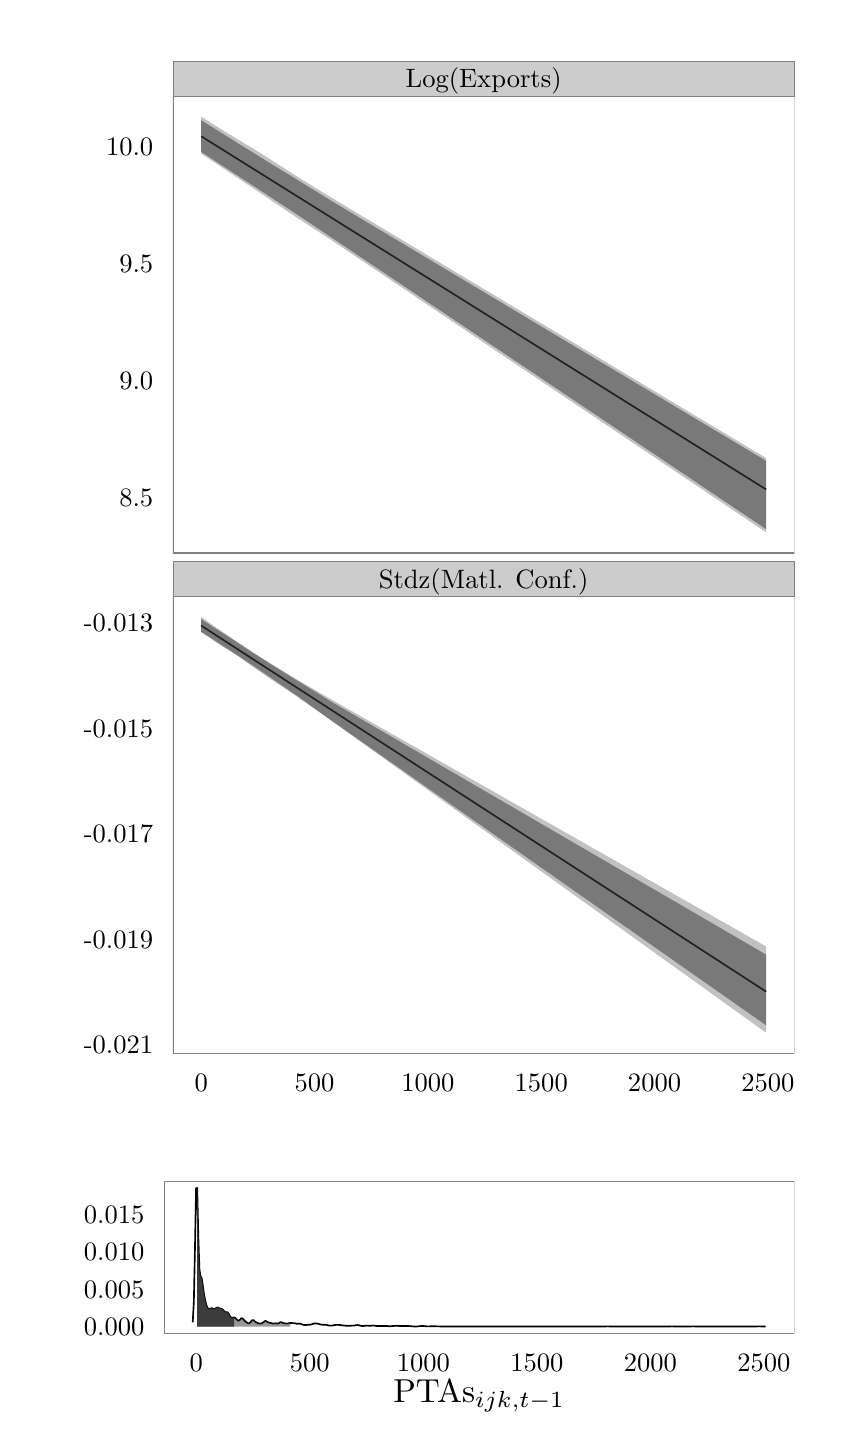
\begin{tikzpicture}[x=1pt,y=1pt]
\definecolor[named]{fillColor}{rgb}{1.00,1.00,1.00}
\path[use as bounding box,fill=fillColor,fill opacity=0.00] (0,0) rectangle (289.08,505.89);
\begin{scope}
\path[clip] (  0.00,101.18) rectangle (289.08,505.89);
\definecolor[named]{drawColor}{rgb}{1.00,1.00,1.00}
\definecolor[named]{fillColor}{rgb}{1.00,1.00,1.00}

\path[draw=drawColor,line width= 0.6pt,line join=round,line cap=round,fill=fillColor] (  0.00,101.18) rectangle (289.08,505.89);
\end{scope}
\begin{scope}
\path[clip] ( 52.48,316.03) rectangle (277.03,481.21);
\definecolor[named]{fillColor}{rgb}{1.00,1.00,1.00}

\path[fill=fillColor] ( 52.48,316.03) rectangle (277.03,481.21);
\definecolor[named]{drawColor}{rgb}{0.00,0.00,0.00}

\path[draw=drawColor,line width= 0.6pt,line join=round] ( 62.69,466.65) --
	( 62.94,466.50) --
	( 63.35,466.24) --
	( 64.08,465.78) --
	( 64.57,465.47) --
	( 65.31,465.01) --
	( 66.54,464.24) --
	( 68.26,463.17) --
	( 70.06,462.04) --
	( 71.70,461.02) --
	( 73.75,459.74) --
	( 76.53,458.00) --
	( 81.12,455.13) --
	( 88.08,450.77) --
	( 96.93,445.24) --
	(109.87,437.15) --
	(266.83,339.03);
\definecolor[named]{fillColor}{rgb}{0.20,0.20,0.20}

\path[fill=fillColor,fill opacity=0.30] ( 62.69,473.70) --
	( 62.94,473.55) --
	( 63.35,473.29) --
	( 64.08,472.84) --
	( 64.57,472.53) --
	( 65.31,472.07) --
	( 66.54,471.30) --
	( 68.26,470.23) --
	( 70.06,469.11) --
	( 71.70,468.09) --
	( 73.75,466.85) --
	( 76.53,465.17) --
	( 81.12,462.40) --
	( 88.08,458.06) --
	( 96.93,452.35) --
	(109.87,444.38) --
	(266.83,350.37) --
	(266.83,323.54) --
	(109.87,429.03) --
	( 96.93,437.47) --
	( 88.08,443.41) --
	( 81.12,448.09) --
	( 76.53,451.17) --
	( 73.75,453.04) --
	( 71.70,454.37) --
	( 70.06,455.47) --
	( 68.26,456.67) --
	( 66.54,457.82) --
	( 65.31,458.64) --
	( 64.57,459.13) --
	( 64.08,459.46) --
	( 63.35,459.95) --
	( 62.94,460.23) --
	( 62.69,460.39) --
	cycle;
\definecolor[named]{fillColor}{rgb}{0.20,0.20,0.20}

\path[fill=fillColor,fill opacity=0.50] ( 62.69,472.42) --
	( 62.94,472.27) --
	( 63.35,472.01) --
	( 64.08,471.55) --
	( 64.57,471.25) --
	( 65.31,470.79) --
	( 66.54,470.02) --
	( 68.26,468.95) --
	( 70.06,467.82) --
	( 71.70,466.80) --
	( 73.75,465.52) --
	( 76.53,463.78) --
	( 81.12,460.94) --
	( 88.08,456.62) --
	( 96.93,451.22) --
	(109.87,443.21) --
	(266.83,349.35) --
	(266.83,324.69) --
	(109.87,430.00) --
	( 96.93,438.67) --
	( 88.08,444.45) --
	( 81.12,449.01) --
	( 76.53,451.98) --
	( 73.75,453.80) --
	( 71.70,455.14) --
	( 70.06,456.20) --
	( 68.26,457.38) --
	( 66.54,458.50) --
	( 65.31,459.31) --
	( 64.57,459.80) --
	( 64.08,460.11) --
	( 63.35,460.58) --
	( 62.94,460.85) --
	( 62.69,461.01) --
	cycle;
\definecolor[named]{drawColor}{rgb}{0.50,0.50,0.50}

\path[draw=drawColor,line width= 0.6pt,line join=round,line cap=round] ( 52.48,316.03) rectangle (277.03,481.21);
\end{scope}
\begin{scope}
\path[clip] ( 52.48,135.21) rectangle (277.03,300.39);
\definecolor[named]{fillColor}{rgb}{1.00,1.00,1.00}

\path[fill=fillColor] ( 52.48,135.21) rectangle (277.03,300.39);
\definecolor[named]{drawColor}{rgb}{0.00,0.00,0.00}

\path[draw=drawColor,line width= 0.6pt,line join=round] ( 62.69,289.82) --
	( 62.94,289.67) --
	( 63.35,289.40) --
	( 64.08,288.92) --
	( 64.57,288.60) --
	( 65.31,288.13) --
	( 66.54,287.33) --
	( 68.26,286.22) --
	( 70.06,285.05) --
	( 71.70,283.99) --
	( 73.75,282.66) --
	( 76.53,280.86) --
	( 81.12,277.88) --
	( 88.08,273.37) --
	( 96.93,267.64) --
	(109.87,259.26) --
	(266.83,157.57);
\definecolor[named]{fillColor}{rgb}{0.20,0.20,0.20}

\path[fill=fillColor,fill opacity=0.30] ( 62.69,292.88) --
	( 62.94,292.73) --
	( 63.35,292.49) --
	( 64.08,291.99) --
	( 64.57,291.64) --
	( 65.31,291.11) --
	( 66.54,290.23) --
	( 68.26,289.02) --
	( 70.06,287.81) --
	( 71.70,286.70) --
	( 73.75,285.31) --
	( 76.53,283.42) --
	( 81.12,280.41) --
	( 88.08,275.97) --
	( 96.93,270.57) --
	(109.87,263.04) --
	(266.83,173.89) --
	(266.83,142.72) --
	(109.87,255.37) --
	( 96.93,264.45) --
	( 88.08,270.33) --
	( 81.12,275.14) --
	( 76.53,278.39) --
	( 73.75,280.32) --
	( 71.70,281.52) --
	( 70.06,282.45) --
	( 68.26,283.65) --
	( 66.54,284.82) --
	( 65.31,285.65) --
	( 64.57,286.15) --
	( 64.08,286.48) --
	( 63.35,286.97) --
	( 62.94,287.22) --
	( 62.69,287.36) --
	cycle;
\definecolor[named]{fillColor}{rgb}{0.20,0.20,0.20}

\path[fill=fillColor,fill opacity=0.50] ( 62.69,292.18) --
	( 62.94,292.01) --
	( 63.35,291.73) --
	( 64.08,291.25) --
	( 64.57,290.93) --
	( 65.31,290.45) --
	( 66.54,289.65) --
	( 68.26,288.54) --
	( 70.06,287.38) --
	( 71.70,286.32) --
	( 73.75,285.00) --
	( 76.53,283.19) --
	( 81.12,280.14) --
	( 88.08,275.72) --
	( 96.93,270.24) --
	(109.87,262.25) --
	(266.83,170.94) --
	(266.83,145.40) --
	(109.87,255.46) --
	( 96.93,264.75) --
	( 88.08,270.83) --
	( 81.12,275.56) --
	( 76.53,278.64) --
	( 73.75,280.40) --
	( 71.70,281.76) --
	( 70.06,282.86) --
	( 68.26,284.03) --
	( 66.54,285.14) --
	( 65.31,285.95) --
	( 64.57,286.41) --
	( 64.08,286.71) --
	( 63.35,287.18) --
	( 62.94,287.45) --
	( 62.69,287.61) --
	cycle;
\definecolor[named]{drawColor}{rgb}{0.50,0.50,0.50}

\path[draw=drawColor,line width= 0.6pt,line join=round,line cap=round] ( 52.48,135.21) rectangle (277.03,300.39);
\end{scope}
\begin{scope}
\path[clip] (  0.00,  0.00) rectangle (289.08,505.89);
\definecolor[named]{drawColor}{rgb}{0.50,0.50,0.50}
\definecolor[named]{fillColor}{rgb}{0.80,0.80,0.80}

\path[draw=drawColor,line width= 0.2pt,line join=round,line cap=round,fill=fillColor] ( 52.48,481.21) rectangle (277.03,493.84);
\definecolor[named]{drawColor}{rgb}{0.00,0.00,0.00}

\node[text=drawColor,anchor=base,inner sep=0pt, outer sep=0pt, scale=  0.96] at (164.76,484.22) {Log(Exports)};
\end{scope}
\begin{scope}
\path[clip] (  0.00,  0.00) rectangle (289.08,505.89);
\definecolor[named]{drawColor}{rgb}{0.50,0.50,0.50}
\definecolor[named]{fillColor}{rgb}{0.80,0.80,0.80}

\path[draw=drawColor,line width= 0.2pt,line join=round,line cap=round,fill=fillColor] ( 52.48,300.39) rectangle (277.03,313.02);
\definecolor[named]{drawColor}{rgb}{0.00,0.00,0.00}

\node[text=drawColor,anchor=base,inner sep=0pt, outer sep=0pt, scale=  0.96] at (164.76,303.40) {Stdz(Matl. Conf.)};
\end{scope}
\begin{scope}
\path[clip] (  0.00,  0.00) rectangle (289.08,505.89);
\definecolor[named]{drawColor}{rgb}{0.00,0.00,0.00}

\node[text=drawColor,anchor=base east,inner sep=0pt, outer sep=0pt, scale=  0.96] at ( 45.37,332.92) {8.5};

\node[text=drawColor,anchor=base east,inner sep=0pt, outer sep=0pt, scale=  0.96] at ( 45.37,375.13) {9.0};

\node[text=drawColor,anchor=base east,inner sep=0pt, outer sep=0pt, scale=  0.96] at ( 45.37,417.35) {9.5};

\node[text=drawColor,anchor=base east,inner sep=0pt, outer sep=0pt, scale=  0.96] at ( 45.37,459.56) {10.0};
\end{scope}
\begin{scope}
\path[clip] (  0.00,  0.00) rectangle (289.08,505.89);
\definecolor[named]{drawColor}{rgb}{0.00,0.00,0.00}

\node[text=drawColor,anchor=base east,inner sep=0pt, outer sep=0pt, scale=  0.96] at ( 45.37,135.03) {-0.021};

\node[text=drawColor,anchor=base east,inner sep=0pt, outer sep=0pt, scale=  0.96] at ( 45.37,173.19) {-0.019};

\node[text=drawColor,anchor=base east,inner sep=0pt, outer sep=0pt, scale=  0.96] at ( 45.37,211.34) {-0.017};

\node[text=drawColor,anchor=base east,inner sep=0pt, outer sep=0pt, scale=  0.96] at ( 45.37,249.50) {-0.015};

\node[text=drawColor,anchor=base east,inner sep=0pt, outer sep=0pt, scale=  0.96] at ( 45.37,287.65) {-0.013};
\end{scope}
\begin{scope}
\path[clip] (  0.00,  0.00) rectangle (289.08,505.89);
\definecolor[named]{drawColor}{rgb}{0.00,0.00,0.00}

\node[text=drawColor,anchor=base,inner sep=0pt, outer sep=0pt, scale=  0.96] at ( 62.69,121.49) {0};

\node[text=drawColor,anchor=base,inner sep=0pt, outer sep=0pt, scale=  0.96] at (103.65,121.49) {500};

\node[text=drawColor,anchor=base,inner sep=0pt, outer sep=0pt, scale=  0.96] at (144.61,121.49) {1000};

\node[text=drawColor,anchor=base,inner sep=0pt, outer sep=0pt, scale=  0.96] at (185.57,121.49) {1500};

\node[text=drawColor,anchor=base,inner sep=0pt, outer sep=0pt, scale=  0.96] at (226.52,121.49) {2000};

\node[text=drawColor,anchor=base,inner sep=0pt, outer sep=0pt, scale=  0.96] at (267.48,121.49) {2500};
\end{scope}
\begin{scope}
\path[clip] (  0.00,  0.00) rectangle (289.08,101.18);
\definecolor[named]{drawColor}{rgb}{1.00,1.00,1.00}
\definecolor[named]{fillColor}{rgb}{1.00,1.00,1.00}

\path[draw=drawColor,line width= 0.6pt,line join=round,line cap=round,fill=fillColor] ( -0.00,  0.00) rectangle (289.08,101.18);
\end{scope}
\begin{scope}
\path[clip] ( 49.28, 34.03) rectangle (277.04, 89.13);
\definecolor[named]{fillColor}{rgb}{1.00,1.00,1.00}

\path[fill=fillColor] ( 49.28, 34.03) rectangle (277.04, 89.13);
\definecolor[named]{drawColor}{rgb}{0.00,0.00,0.00}

\path[draw=drawColor,line width= 0.6pt,line join=round] ( 59.64, 38.05) --
	( 60.04, 45.39) --
	( 60.45, 64.85) --
	( 60.85, 86.49) --
	( 61.26, 86.63) --
	( 61.66, 69.17) --
	( 62.07, 57.11) --
	( 62.47, 54.76) --
	( 62.88, 53.97) --
	( 63.28, 51.42) --
	( 63.69, 48.50) --
	( 64.09, 46.23) --
	( 64.50, 44.54) --
	( 64.90, 43.44) --
	( 65.31, 43.00) --
	( 65.71, 42.85) --
	( 66.12, 43.03) --
	( 66.52, 43.25) --
	( 66.93, 42.98) --
	( 67.33, 42.78) --
	( 67.74, 42.97) --
	( 68.15, 43.27) --
	( 68.55, 43.45) --
	( 68.96, 43.34) --
	( 69.36, 43.10) --
	( 69.77, 42.99) --
	( 70.17, 42.90) --
	( 70.58, 42.58) --
	( 70.98, 42.09) --
	( 71.39, 41.76) --
	( 71.79, 41.75) --
	( 72.20, 41.71) --
	( 72.60, 41.19) --
	( 73.01, 40.38) --
	( 73.41, 39.86) --
	( 73.82, 39.74) --
	( 74.22, 39.79) --
	( 74.63, 39.79) --
	( 75.03, 39.62) --
	( 75.44, 39.22) --
	( 75.84, 38.78) --
	( 76.25, 38.63) --
	( 76.65, 38.91) --
	( 77.06, 39.40) --
	( 77.46, 39.57) --
	( 77.87, 39.24) --
	( 78.27, 38.74) --
	( 78.68, 38.34) --
	( 79.09, 38.05) --
	( 79.49, 37.81) --
	( 79.90, 37.72) --
	( 80.30, 37.87) --
	( 80.71, 38.33) --
	( 81.11, 38.84) --
	( 81.52, 38.88) --
	( 81.92, 38.51) --
	( 82.33, 38.20) --
	( 82.73, 37.99) --
	( 83.14, 37.79) --
	( 83.54, 37.66) --
	( 83.95, 37.62) --
	( 84.35, 37.65) --
	( 84.76, 37.79) --
	( 85.16, 38.04) --
	( 85.57, 38.41) --
	( 85.97, 38.60) --
	( 86.38, 38.39) --
	( 86.78, 38.11) --
	( 87.19, 37.98) --
	( 87.59, 37.88) --
	( 88.00, 37.77) --
	( 88.40, 37.67) --
	( 88.81, 37.64) --
	( 89.21, 37.69) --
	( 89.62, 37.71) --
	( 90.02, 37.64) --
	( 90.43, 37.64) --
	( 90.84, 37.81) --
	( 91.24, 38.06) --
	( 91.65, 38.11) --
	( 92.05, 37.92) --
	( 92.46, 37.76) --
	( 92.86, 37.72) --
	( 93.27, 37.65) --
	( 93.67, 37.58) --
	( 94.08, 37.64) --
	( 94.48, 37.78) --
	( 94.89, 37.84) --
	( 95.29, 37.80) --
	( 95.70, 37.78) --
	( 96.10, 37.79) --
	( 96.51, 37.75) --
	( 96.91, 37.64) --
	( 97.32, 37.53) --
	( 97.72, 37.54) --
	( 98.13, 37.61) --
	( 98.53, 37.56) --
	( 98.94, 37.39) --
	( 99.34, 37.23) --
	( 99.75, 37.13) --
	(100.15, 37.11) --
	(100.56, 37.11) --
	(100.96, 37.14) --
	(101.37, 37.17) --
	(101.78, 37.19) --
	(102.18, 37.23) --
	(102.59, 37.33) --
	(102.99, 37.49) --
	(103.40, 37.62) --
	(103.80, 37.65) --
	(104.21, 37.62) --
	(104.61, 37.61) --
	(105.02, 37.53) --
	(105.42, 37.39) --
	(105.83, 37.28) --
	(106.23, 37.23) --
	(106.64, 37.20) --
	(107.04, 37.20) --
	(107.45, 37.21) --
	(107.85, 37.16) --
	(108.26, 37.05) --
	(108.66, 36.93) --
	(109.07, 36.88) --
	(109.47, 36.87) --
	(109.88, 36.89) --
	(110.28, 36.96) --
	(110.69, 37.05) --
	(111.09, 37.11) --
	(111.50, 37.13) --
	(111.90, 37.13) --
	(112.31, 37.13) --
	(112.71, 37.12) --
	(113.12, 37.08) --
	(113.53, 36.99) --
	(113.93, 36.93) --
	(114.34, 36.91) --
	(114.74, 36.86) --
	(115.15, 36.82) --
	(115.55, 36.82) --
	(115.96, 36.85) --
	(116.36, 36.85) --
	(116.77, 36.85) --
	(117.17, 36.86) --
	(117.58, 36.88) --
	(117.98, 36.91) --
	(118.39, 36.99) --
	(118.79, 37.06) --
	(119.20, 37.08) --
	(119.60, 37.03) --
	(120.01, 36.93) --
	(120.41, 36.82) --
	(120.82, 36.75) --
	(121.22, 36.75) --
	(121.63, 36.79) --
	(122.03, 36.84) --
	(122.44, 36.86) --
	(122.84, 36.87) --
	(123.25, 36.85) --
	(123.65, 36.82) --
	(124.06, 36.83) --
	(124.47, 36.88) --
	(124.87, 36.90) --
	(125.28, 36.87) --
	(125.68, 36.80) --
	(126.09, 36.74) --
	(126.49, 36.72) --
	(126.90, 36.72) --
	(127.30, 36.71) --
	(127.71, 36.71) --
	(128.11, 36.72) --
	(128.52, 36.74) --
	(128.92, 36.76) --
	(129.33, 36.76) --
	(129.73, 36.75) --
	(130.14, 36.71) --
	(130.54, 36.67) --
	(130.95, 36.65) --
	(131.35, 36.68) --
	(131.76, 36.73) --
	(132.16, 36.76) --
	(132.57, 36.77) --
	(132.97, 36.80) --
	(133.38, 36.81) --
	(133.78, 36.78) --
	(134.19, 36.76) --
	(134.59, 36.74) --
	(135.00, 36.73) --
	(135.40, 36.73) --
	(135.81, 36.73) --
	(136.22, 36.72) --
	(136.62, 36.73) --
	(137.03, 36.75) --
	(137.43, 36.73) --
	(137.84, 36.71) --
	(138.24, 36.69) --
	(138.65, 36.64) --
	(139.05, 36.60) --
	(139.46, 36.58) --
	(139.86, 36.57) --
	(140.27, 36.57) --
	(140.67, 36.59) --
	(141.08, 36.61) --
	(141.48, 36.65) --
	(141.89, 36.71) --
	(142.29, 36.74) --
	(142.70, 36.73) --
	(143.10, 36.72) --
	(143.51, 36.69) --
	(143.91, 36.64) --
	(144.32, 36.60) --
	(144.72, 36.60) --
	(145.13, 36.61) --
	(145.53, 36.63) --
	(145.94, 36.64) --
	(146.34, 36.64) --
	(146.75, 36.64) --
	(147.16, 36.64) --
	(147.56, 36.62) --
	(147.97, 36.61) --
	(148.37, 36.60) --
	(148.78, 36.59) --
	(149.18, 36.57) --
	(149.59, 36.57) --
	(149.99, 36.57) --
	(150.40, 36.58) --
	(150.80, 36.58) --
	(151.21, 36.57) --
	(151.61, 36.57) --
	(152.02, 36.57) --
	(152.42, 36.56) --
	(152.83, 36.55) --
	(153.23, 36.54) --
	(153.64, 36.54) --
	(154.04, 36.54) --
	(154.45, 36.54) --
	(154.85, 36.54) --
	(155.26, 36.54) --
	(155.66, 36.54) --
	(156.07, 36.54) --
	(156.47, 36.54) --
	(156.88, 36.54) --
	(157.28, 36.54) --
	(157.69, 36.54) --
	(158.09, 36.54) --
	(158.50, 36.54) --
	(158.91, 36.54) --
	(159.31, 36.54) --
	(159.72, 36.54) --
	(160.12, 36.54) --
	(160.53, 36.54) --
	(160.93, 36.54) --
	(161.34, 36.54) --
	(161.74, 36.54) --
	(162.15, 36.55) --
	(162.55, 36.56) --
	(162.96, 36.56) --
	(163.36, 36.57) --
	(163.77, 36.56) --
	(164.17, 36.56) --
	(164.58, 36.55) --
	(164.98, 36.55) --
	(165.39, 36.54) --
	(165.79, 36.54) --
	(166.20, 36.55) --
	(166.60, 36.56) --
	(167.01, 36.58) --
	(167.41, 36.58) --
	(167.82, 36.58) --
	(168.22, 36.57) --
	(168.63, 36.56) --
	(169.03, 36.56) --
	(169.44, 36.55) --
	(169.85, 36.55) --
	(170.25, 36.55) --
	(170.66, 36.55) --
	(171.06, 36.55) --
	(171.47, 36.55) --
	(171.87, 36.55) --
	(172.28, 36.54) --
	(172.68, 36.54) --
	(173.09, 36.54) --
	(173.49, 36.54) --
	(173.90, 36.54) --
	(174.30, 36.54) --
	(174.71, 36.54) --
	(175.11, 36.54) --
	(175.52, 36.54) --
	(175.92, 36.54) --
	(176.33, 36.54) --
	(176.73, 36.54) --
	(177.14, 36.54) --
	(177.54, 36.54) --
	(177.95, 36.54) --
	(178.35, 36.54) --
	(178.76, 36.54) --
	(179.16, 36.54) --
	(179.57, 36.54) --
	(179.97, 36.54) --
	(180.38, 36.54) --
	(180.78, 36.54) --
	(181.19, 36.54) --
	(181.60, 36.54) --
	(182.00, 36.54) --
	(182.41, 36.54) --
	(182.81, 36.54) --
	(183.22, 36.54) --
	(183.62, 36.54) --
	(184.03, 36.54) --
	(184.43, 36.54) --
	(184.84, 36.54) --
	(185.24, 36.55) --
	(185.65, 36.55) --
	(186.05, 36.55) --
	(186.46, 36.54) --
	(186.86, 36.54) --
	(187.27, 36.54) --
	(187.67, 36.55) --
	(188.08, 36.55) --
	(188.48, 36.55) --
	(188.89, 36.56) --
	(189.29, 36.56) --
	(189.70, 36.56) --
	(190.10, 36.56) --
	(190.51, 36.55) --
	(190.91, 36.55) --
	(191.32, 36.54) --
	(191.72, 36.54) --
	(192.13, 36.54) --
	(192.54, 36.54) --
	(192.94, 36.54) --
	(193.35, 36.54) --
	(193.75, 36.54) --
	(194.16, 36.54) --
	(194.56, 36.54) --
	(194.97, 36.54) --
	(195.37, 36.54) --
	(195.78, 36.54) --
	(196.18, 36.54) --
	(196.59, 36.54) --
	(196.99, 36.54) --
	(197.40, 36.54) --
	(197.80, 36.54) --
	(198.21, 36.54) --
	(198.61, 36.54) --
	(199.02, 36.54) --
	(199.42, 36.54) --
	(199.83, 36.54) --
	(200.23, 36.54) --
	(200.64, 36.54) --
	(201.04, 36.54) --
	(201.45, 36.54) --
	(201.85, 36.54) --
	(202.26, 36.54) --
	(202.66, 36.54) --
	(203.07, 36.54) --
	(203.47, 36.54) --
	(203.88, 36.54) --
	(204.29, 36.54) --
	(204.69, 36.54) --
	(205.10, 36.54) --
	(205.50, 36.54) --
	(205.91, 36.54) --
	(206.31, 36.55) --
	(206.72, 36.56) --
	(207.12, 36.57) --
	(207.53, 36.58) --
	(207.93, 36.57) --
	(208.34, 36.57) --
	(208.74, 36.57) --
	(209.15, 36.59) --
	(209.55, 36.60) --
	(209.96, 36.59) --
	(210.36, 36.57) --
	(210.77, 36.55) --
	(211.17, 36.54) --
	(211.58, 36.54) --
	(211.98, 36.54) --
	(212.39, 36.54) --
	(212.79, 36.54) --
	(213.20, 36.54) --
	(213.60, 36.54) --
	(214.01, 36.54) --
	(214.41, 36.54) --
	(214.82, 36.54) --
	(215.23, 36.54) --
	(215.63, 36.54) --
	(216.04, 36.54) --
	(216.44, 36.54) --
	(216.85, 36.54) --
	(217.25, 36.54) --
	(217.66, 36.54) --
	(218.06, 36.54) --
	(218.47, 36.54) --
	(218.87, 36.54) --
	(219.28, 36.54) --
	(219.68, 36.54) --
	(220.09, 36.54) --
	(220.49, 36.54) --
	(220.90, 36.54) --
	(221.30, 36.54) --
	(221.71, 36.54) --
	(222.11, 36.54) --
	(222.52, 36.54) --
	(222.92, 36.54) --
	(223.33, 36.54) --
	(223.73, 36.54) --
	(224.14, 36.54) --
	(224.54, 36.55) --
	(224.95, 36.55) --
	(225.35, 36.55) --
	(225.76, 36.54) --
	(226.16, 36.54) --
	(226.57, 36.54) --
	(226.98, 36.54) --
	(227.38, 36.54) --
	(227.79, 36.54) --
	(228.19, 36.54) --
	(228.60, 36.54) --
	(229.00, 36.54) --
	(229.41, 36.55) --
	(229.81, 36.56) --
	(230.22, 36.57) --
	(230.62, 36.57) --
	(231.03, 36.56) --
	(231.43, 36.56) --
	(231.84, 36.57) --
	(232.24, 36.58) --
	(232.65, 36.59) --
	(233.05, 36.59) --
	(233.46, 36.58) --
	(233.86, 36.56) --
	(234.27, 36.55) --
	(234.67, 36.54) --
	(235.08, 36.54) --
	(235.48, 36.54) --
	(235.89, 36.54) --
	(236.29, 36.54) --
	(236.70, 36.54) --
	(237.10, 36.54) --
	(237.51, 36.54) --
	(237.92, 36.54) --
	(238.32, 36.54) --
	(238.73, 36.55) --
	(239.13, 36.56) --
	(239.54, 36.57) --
	(239.94, 36.59) --
	(240.35, 36.61) --
	(240.75, 36.60) --
	(241.16, 36.57) --
	(241.56, 36.55) --
	(241.97, 36.54) --
	(242.37, 36.54) --
	(242.78, 36.54) --
	(243.18, 36.54) --
	(243.59, 36.54) --
	(243.99, 36.54) --
	(244.40, 36.54) --
	(244.80, 36.54) --
	(245.21, 36.54) --
	(245.61, 36.54) --
	(246.02, 36.54) --
	(246.42, 36.54) --
	(246.83, 36.54) --
	(247.23, 36.54) --
	(247.64, 36.54) --
	(248.04, 36.54) --
	(248.45, 36.54) --
	(248.85, 36.54) --
	(249.26, 36.54) --
	(249.67, 36.54) --
	(250.07, 36.54) --
	(250.48, 36.54) --
	(250.88, 36.54) --
	(251.29, 36.54) --
	(251.69, 36.54) --
	(252.10, 36.54) --
	(252.50, 36.54) --
	(252.91, 36.54) --
	(253.31, 36.54) --
	(253.72, 36.54) --
	(254.12, 36.54) --
	(254.53, 36.54) --
	(254.93, 36.54) --
	(255.34, 36.54) --
	(255.74, 36.55) --
	(256.15, 36.55) --
	(256.55, 36.55) --
	(256.96, 36.55) --
	(257.36, 36.54) --
	(257.77, 36.54) --
	(258.17, 36.54) --
	(258.58, 36.54) --
	(258.98, 36.54) --
	(259.39, 36.54) --
	(259.79, 36.54) --
	(260.20, 36.54) --
	(260.61, 36.54) --
	(261.01, 36.54) --
	(261.42, 36.54) --
	(261.82, 36.54) --
	(262.23, 36.54) --
	(262.63, 36.55) --
	(263.04, 36.56) --
	(263.44, 36.57) --
	(263.85, 36.60) --
	(264.25, 36.61) --
	(264.66, 36.60) --
	(265.06, 36.58) --
	(265.47, 36.56) --
	(265.87, 36.55) --
	(266.28, 36.54) --
	(266.68, 36.54);
\definecolor[named]{fillColor}{rgb}{0.20,0.20,0.20}

\path[fill=fillColor,fill opacity=0.50] ( 61.26, 86.63) --
	( 61.66, 69.17) --
	( 62.07, 57.11) --
	( 62.47, 54.76) --
	( 62.88, 53.97) --
	( 63.28, 51.42) --
	( 63.69, 48.50) --
	( 64.09, 46.23) --
	( 64.50, 44.54) --
	( 64.90, 43.44) --
	( 65.31, 43.00) --
	( 65.71, 42.85) --
	( 66.12, 43.03) --
	( 66.52, 43.25) --
	( 66.93, 42.98) --
	( 67.33, 42.78) --
	( 67.74, 42.97) --
	( 68.15, 43.27) --
	( 68.55, 43.45) --
	( 68.96, 43.34) --
	( 69.36, 43.10) --
	( 69.77, 42.99) --
	( 70.17, 42.90) --
	( 70.58, 42.58) --
	( 70.98, 42.09) --
	( 71.39, 41.76) --
	( 71.79, 41.75) --
	( 72.20, 41.71) --
	( 72.60, 41.19) --
	( 73.01, 40.38) --
	( 73.41, 39.86) --
	( 73.82, 39.74) --
	( 74.22, 39.79) --
	( 74.63, 39.79) --
	( 75.03, 39.62) --
	( 75.44, 39.22) --
	( 75.84, 38.78) --
	( 76.25, 38.63) --
	( 76.65, 38.91) --
	( 77.06, 39.40) --
	( 77.46, 39.57) --
	( 77.87, 39.24) --
	( 78.27, 38.74) --
	( 78.68, 38.34) --
	( 79.09, 38.05) --
	( 79.49, 37.81) --
	( 79.90, 37.72) --
	( 80.30, 37.87) --
	( 80.71, 38.33) --
	( 81.11, 38.84) --
	( 81.52, 38.88) --
	( 81.92, 38.51) --
	( 82.33, 38.20) --
	( 82.73, 37.99) --
	( 83.14, 37.79) --
	( 83.54, 37.66) --
	( 83.95, 37.62) --
	( 84.35, 37.65) --
	( 84.76, 37.79) --
	( 85.16, 38.04) --
	( 85.57, 38.41) --
	( 85.97, 38.60) --
	( 86.38, 38.39) --
	( 86.78, 38.11) --
	( 87.19, 37.98) --
	( 87.59, 37.88) --
	( 88.00, 37.77) --
	( 88.40, 37.67) --
	( 88.81, 37.64) --
	( 89.21, 37.69) --
	( 89.62, 37.71) --
	( 90.02, 37.64) --
	( 90.43, 37.64) --
	( 90.84, 37.81) --
	( 91.24, 38.06) --
	( 91.65, 38.11) --
	( 92.05, 37.92) --
	( 92.46, 37.76) --
	( 92.86, 37.72) --
	( 93.27, 37.65) --
	( 93.67, 37.58) --
	( 94.08, 37.64) --
	( 94.48, 37.78) --
	( 94.89, 37.84) --
	( 94.89, 36.54) --
	( 94.48, 36.54) --
	( 94.08, 36.54) --
	( 93.67, 36.54) --
	( 93.27, 36.54) --
	( 92.86, 36.54) --
	( 92.46, 36.54) --
	( 92.05, 36.54) --
	( 91.65, 36.54) --
	( 91.24, 36.54) --
	( 90.84, 36.54) --
	( 90.43, 36.54) --
	( 90.02, 36.54) --
	( 89.62, 36.54) --
	( 89.21, 36.54) --
	( 88.81, 36.54) --
	( 88.40, 36.54) --
	( 88.00, 36.54) --
	( 87.59, 36.54) --
	( 87.19, 36.54) --
	( 86.78, 36.54) --
	( 86.38, 36.54) --
	( 85.97, 36.54) --
	( 85.57, 36.54) --
	( 85.16, 36.54) --
	( 84.76, 36.54) --
	( 84.35, 36.54) --
	( 83.95, 36.54) --
	( 83.54, 36.54) --
	( 83.14, 36.54) --
	( 82.73, 36.54) --
	( 82.33, 36.54) --
	( 81.92, 36.54) --
	( 81.52, 36.54) --
	( 81.11, 36.54) --
	( 80.71, 36.54) --
	( 80.30, 36.54) --
	( 79.90, 36.54) --
	( 79.49, 36.54) --
	( 79.09, 36.54) --
	( 78.68, 36.54) --
	( 78.27, 36.54) --
	( 77.87, 36.54) --
	( 77.46, 36.54) --
	( 77.06, 36.54) --
	( 76.65, 36.54) --
	( 76.25, 36.54) --
	( 75.84, 36.54) --
	( 75.44, 36.54) --
	( 75.03, 36.54) --
	( 74.63, 36.54) --
	( 74.22, 36.54) --
	( 73.82, 36.54) --
	( 73.41, 36.54) --
	( 73.01, 36.54) --
	( 72.60, 36.54) --
	( 72.20, 36.54) --
	( 71.79, 36.54) --
	( 71.39, 36.54) --
	( 70.98, 36.54) --
	( 70.58, 36.54) --
	( 70.17, 36.54) --
	( 69.77, 36.54) --
	( 69.36, 36.54) --
	( 68.96, 36.54) --
	( 68.55, 36.54) --
	( 68.15, 36.54) --
	( 67.74, 36.54) --
	( 67.33, 36.54) --
	( 66.93, 36.54) --
	( 66.52, 36.54) --
	( 66.12, 36.54) --
	( 65.71, 36.54) --
	( 65.31, 36.54) --
	( 64.90, 36.54) --
	( 64.50, 36.54) --
	( 64.09, 36.54) --
	( 63.69, 36.54) --
	( 63.28, 36.54) --
	( 62.88, 36.54) --
	( 62.47, 36.54) --
	( 62.07, 36.54) --
	( 61.66, 36.54) --
	( 61.26, 36.54) --
	cycle;
\definecolor[named]{fillColor}{rgb}{0.20,0.20,0.20}

\path[fill=fillColor,fill opacity=0.90] ( 61.26, 86.63) --
	( 61.66, 69.17) --
	( 62.07, 57.11) --
	( 62.47, 54.76) --
	( 62.88, 53.97) --
	( 63.28, 51.42) --
	( 63.69, 48.50) --
	( 64.09, 46.23) --
	( 64.50, 44.54) --
	( 64.90, 43.44) --
	( 65.31, 43.00) --
	( 65.71, 42.85) --
	( 66.12, 43.03) --
	( 66.52, 43.25) --
	( 66.93, 42.98) --
	( 67.33, 42.78) --
	( 67.74, 42.97) --
	( 68.15, 43.27) --
	( 68.55, 43.45) --
	( 68.96, 43.34) --
	( 69.36, 43.10) --
	( 69.77, 42.99) --
	( 70.17, 42.90) --
	( 70.58, 42.58) --
	( 70.98, 42.09) --
	( 71.39, 41.76) --
	( 71.79, 41.75) --
	( 72.20, 41.71) --
	( 72.60, 41.19) --
	( 73.01, 40.38) --
	( 73.41, 39.86) --
	( 73.82, 39.74) --
	( 74.22, 39.79) --
	( 74.63, 39.79) --
	( 74.63, 36.54) --
	( 74.22, 36.54) --
	( 73.82, 36.54) --
	( 73.41, 36.54) --
	( 73.01, 36.54) --
	( 72.60, 36.54) --
	( 72.20, 36.54) --
	( 71.79, 36.54) --
	( 71.39, 36.54) --
	( 70.98, 36.54) --
	( 70.58, 36.54) --
	( 70.17, 36.54) --
	( 69.77, 36.54) --
	( 69.36, 36.54) --
	( 68.96, 36.54) --
	( 68.55, 36.54) --
	( 68.15, 36.54) --
	( 67.74, 36.54) --
	( 67.33, 36.54) --
	( 66.93, 36.54) --
	( 66.52, 36.54) --
	( 66.12, 36.54) --
	( 65.71, 36.54) --
	( 65.31, 36.54) --
	( 64.90, 36.54) --
	( 64.50, 36.54) --
	( 64.09, 36.54) --
	( 63.69, 36.54) --
	( 63.28, 36.54) --
	( 62.88, 36.54) --
	( 62.47, 36.54) --
	( 62.07, 36.54) --
	( 61.66, 36.54) --
	( 61.26, 36.54) --
	cycle;
\definecolor[named]{drawColor}{rgb}{0.50,0.50,0.50}

\path[draw=drawColor,line width= 0.6pt,line join=round,line cap=round] ( 49.28, 34.03) rectangle (277.04, 89.13);
\end{scope}
\begin{scope}
\path[clip] (  0.00,  0.00) rectangle (289.08,505.89);
\definecolor[named]{drawColor}{rgb}{0.00,0.00,0.00}

\node[text=drawColor,anchor=base east,inner sep=0pt, outer sep=0pt, scale=  0.96] at ( 42.17, 33.23) {0.000};

\node[text=drawColor,anchor=base east,inner sep=0pt, outer sep=0pt, scale=  0.96] at ( 42.17, 46.79) {0.005};

\node[text=drawColor,anchor=base east,inner sep=0pt, outer sep=0pt, scale=  0.96] at ( 42.17, 60.35) {0.010};

\node[text=drawColor,anchor=base east,inner sep=0pt, outer sep=0pt, scale=  0.96] at ( 42.17, 73.92) {0.015};
\end{scope}
\begin{scope}
\path[clip] (  0.00,  0.00) rectangle (289.08,505.89);
\definecolor[named]{drawColor}{rgb}{0.00,0.00,0.00}

\node[text=drawColor,anchor=base,inner sep=0pt, outer sep=0pt, scale=  0.96] at ( 60.93, 20.31) {0};

\node[text=drawColor,anchor=base,inner sep=0pt, outer sep=0pt, scale=  0.96] at (101.95, 20.31) {500};

\node[text=drawColor,anchor=base,inner sep=0pt, outer sep=0pt, scale=  0.96] at (142.98, 20.31) {1000};

\node[text=drawColor,anchor=base,inner sep=0pt, outer sep=0pt, scale=  0.96] at (184.00, 20.31) {1500};

\node[text=drawColor,anchor=base,inner sep=0pt, outer sep=0pt, scale=  0.96] at (225.02, 20.31) {2000};

\node[text=drawColor,anchor=base,inner sep=0pt, outer sep=0pt, scale=  0.96] at (266.04, 20.31) {2500};
\end{scope}
\begin{scope}
\path[clip] (  0.00,  0.00) rectangle (289.08,505.89);
\definecolor[named]{drawColor}{rgb}{0.00,0.00,0.00}

\node[text=drawColor,anchor=base,inner sep=0pt, outer sep=0pt, scale=  1.20] at (163.16,  9.03) {PTAs$_{ijk, t-1}$};
\end{scope}
\end{tikzpicture}
}  &
      \resizebox{.38\textwidth}{!}{% Created by tikzDevice version 0.7.0 on 2015-07-01 08:58:18
% !TEX encoding = UTF-8 Unicode
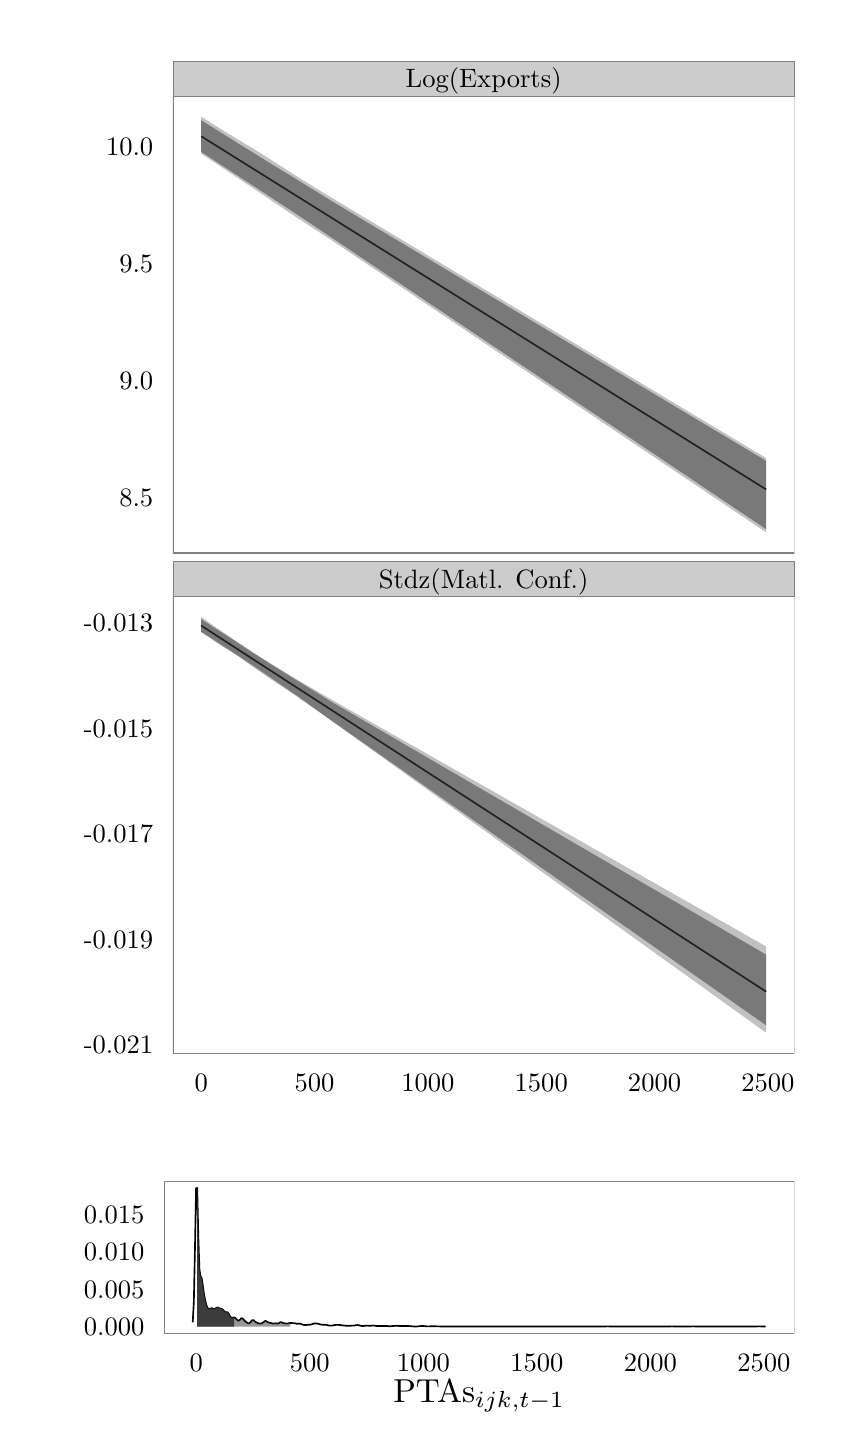
\begin{tikzpicture}[x=1pt,y=1pt]
\definecolor[named]{fillColor}{rgb}{1.00,1.00,1.00}
\path[use as bounding box,fill=fillColor,fill opacity=0.00] (0,0) rectangle (289.08,505.89);
\begin{scope}
\path[clip] (  0.00,101.18) rectangle (289.08,505.89);
\definecolor[named]{drawColor}{rgb}{1.00,1.00,1.00}
\definecolor[named]{fillColor}{rgb}{1.00,1.00,1.00}

\path[draw=drawColor,line width= 0.6pt,line join=round,line cap=round,fill=fillColor] (  0.00,101.18) rectangle (289.08,505.89);
\end{scope}
\begin{scope}
\path[clip] ( 52.48,316.03) rectangle (277.03,481.21);
\definecolor[named]{fillColor}{rgb}{1.00,1.00,1.00}

\path[fill=fillColor] ( 52.48,316.03) rectangle (277.03,481.21);
\definecolor[named]{drawColor}{rgb}{0.00,0.00,0.00}

\path[draw=drawColor,line width= 0.6pt,line join=round] ( 62.69,466.65) --
	( 62.94,466.50) --
	( 63.35,466.24) --
	( 64.08,465.78) --
	( 64.57,465.47) --
	( 65.31,465.01) --
	( 66.54,464.24) --
	( 68.26,463.17) --
	( 70.06,462.04) --
	( 71.70,461.02) --
	( 73.75,459.74) --
	( 76.53,458.00) --
	( 81.12,455.13) --
	( 88.08,450.77) --
	( 96.93,445.24) --
	(109.87,437.15) --
	(266.83,339.03);
\definecolor[named]{fillColor}{rgb}{0.20,0.20,0.20}

\path[fill=fillColor,fill opacity=0.30] ( 62.69,473.70) --
	( 62.94,473.55) --
	( 63.35,473.29) --
	( 64.08,472.84) --
	( 64.57,472.53) --
	( 65.31,472.07) --
	( 66.54,471.30) --
	( 68.26,470.23) --
	( 70.06,469.11) --
	( 71.70,468.09) --
	( 73.75,466.85) --
	( 76.53,465.17) --
	( 81.12,462.40) --
	( 88.08,458.06) --
	( 96.93,452.35) --
	(109.87,444.38) --
	(266.83,350.37) --
	(266.83,323.54) --
	(109.87,429.03) --
	( 96.93,437.47) --
	( 88.08,443.41) --
	( 81.12,448.09) --
	( 76.53,451.17) --
	( 73.75,453.04) --
	( 71.70,454.37) --
	( 70.06,455.47) --
	( 68.26,456.67) --
	( 66.54,457.82) --
	( 65.31,458.64) --
	( 64.57,459.13) --
	( 64.08,459.46) --
	( 63.35,459.95) --
	( 62.94,460.23) --
	( 62.69,460.39) --
	cycle;
\definecolor[named]{fillColor}{rgb}{0.20,0.20,0.20}

\path[fill=fillColor,fill opacity=0.50] ( 62.69,472.42) --
	( 62.94,472.27) --
	( 63.35,472.01) --
	( 64.08,471.55) --
	( 64.57,471.25) --
	( 65.31,470.79) --
	( 66.54,470.02) --
	( 68.26,468.95) --
	( 70.06,467.82) --
	( 71.70,466.80) --
	( 73.75,465.52) --
	( 76.53,463.78) --
	( 81.12,460.94) --
	( 88.08,456.62) --
	( 96.93,451.22) --
	(109.87,443.21) --
	(266.83,349.35) --
	(266.83,324.69) --
	(109.87,430.00) --
	( 96.93,438.67) --
	( 88.08,444.45) --
	( 81.12,449.01) --
	( 76.53,451.98) --
	( 73.75,453.80) --
	( 71.70,455.14) --
	( 70.06,456.20) --
	( 68.26,457.38) --
	( 66.54,458.50) --
	( 65.31,459.31) --
	( 64.57,459.80) --
	( 64.08,460.11) --
	( 63.35,460.58) --
	( 62.94,460.85) --
	( 62.69,461.01) --
	cycle;
\definecolor[named]{drawColor}{rgb}{0.50,0.50,0.50}

\path[draw=drawColor,line width= 0.6pt,line join=round,line cap=round] ( 52.48,316.03) rectangle (277.03,481.21);
\end{scope}
\begin{scope}
\path[clip] ( 52.48,135.21) rectangle (277.03,300.39);
\definecolor[named]{fillColor}{rgb}{1.00,1.00,1.00}

\path[fill=fillColor] ( 52.48,135.21) rectangle (277.03,300.39);
\definecolor[named]{drawColor}{rgb}{0.00,0.00,0.00}

\path[draw=drawColor,line width= 0.6pt,line join=round] ( 62.69,289.82) --
	( 62.94,289.67) --
	( 63.35,289.40) --
	( 64.08,288.92) --
	( 64.57,288.60) --
	( 65.31,288.13) --
	( 66.54,287.33) --
	( 68.26,286.22) --
	( 70.06,285.05) --
	( 71.70,283.99) --
	( 73.75,282.66) --
	( 76.53,280.86) --
	( 81.12,277.88) --
	( 88.08,273.37) --
	( 96.93,267.64) --
	(109.87,259.26) --
	(266.83,157.57);
\definecolor[named]{fillColor}{rgb}{0.20,0.20,0.20}

\path[fill=fillColor,fill opacity=0.30] ( 62.69,292.88) --
	( 62.94,292.73) --
	( 63.35,292.49) --
	( 64.08,291.99) --
	( 64.57,291.64) --
	( 65.31,291.11) --
	( 66.54,290.23) --
	( 68.26,289.02) --
	( 70.06,287.81) --
	( 71.70,286.70) --
	( 73.75,285.31) --
	( 76.53,283.42) --
	( 81.12,280.41) --
	( 88.08,275.97) --
	( 96.93,270.57) --
	(109.87,263.04) --
	(266.83,173.89) --
	(266.83,142.72) --
	(109.87,255.37) --
	( 96.93,264.45) --
	( 88.08,270.33) --
	( 81.12,275.14) --
	( 76.53,278.39) --
	( 73.75,280.32) --
	( 71.70,281.52) --
	( 70.06,282.45) --
	( 68.26,283.65) --
	( 66.54,284.82) --
	( 65.31,285.65) --
	( 64.57,286.15) --
	( 64.08,286.48) --
	( 63.35,286.97) --
	( 62.94,287.22) --
	( 62.69,287.36) --
	cycle;
\definecolor[named]{fillColor}{rgb}{0.20,0.20,0.20}

\path[fill=fillColor,fill opacity=0.50] ( 62.69,292.18) --
	( 62.94,292.01) --
	( 63.35,291.73) --
	( 64.08,291.25) --
	( 64.57,290.93) --
	( 65.31,290.45) --
	( 66.54,289.65) --
	( 68.26,288.54) --
	( 70.06,287.38) --
	( 71.70,286.32) --
	( 73.75,285.00) --
	( 76.53,283.19) --
	( 81.12,280.14) --
	( 88.08,275.72) --
	( 96.93,270.24) --
	(109.87,262.25) --
	(266.83,170.94) --
	(266.83,145.40) --
	(109.87,255.46) --
	( 96.93,264.75) --
	( 88.08,270.83) --
	( 81.12,275.56) --
	( 76.53,278.64) --
	( 73.75,280.40) --
	( 71.70,281.76) --
	( 70.06,282.86) --
	( 68.26,284.03) --
	( 66.54,285.14) --
	( 65.31,285.95) --
	( 64.57,286.41) --
	( 64.08,286.71) --
	( 63.35,287.18) --
	( 62.94,287.45) --
	( 62.69,287.61) --
	cycle;
\definecolor[named]{drawColor}{rgb}{0.50,0.50,0.50}

\path[draw=drawColor,line width= 0.6pt,line join=round,line cap=round] ( 52.48,135.21) rectangle (277.03,300.39);
\end{scope}
\begin{scope}
\path[clip] (  0.00,  0.00) rectangle (289.08,505.89);
\definecolor[named]{drawColor}{rgb}{0.50,0.50,0.50}
\definecolor[named]{fillColor}{rgb}{0.80,0.80,0.80}

\path[draw=drawColor,line width= 0.2pt,line join=round,line cap=round,fill=fillColor] ( 52.48,481.21) rectangle (277.03,493.84);
\definecolor[named]{drawColor}{rgb}{0.00,0.00,0.00}

\node[text=drawColor,anchor=base,inner sep=0pt, outer sep=0pt, scale=  0.96] at (164.76,484.22) {Log(Exports)};
\end{scope}
\begin{scope}
\path[clip] (  0.00,  0.00) rectangle (289.08,505.89);
\definecolor[named]{drawColor}{rgb}{0.50,0.50,0.50}
\definecolor[named]{fillColor}{rgb}{0.80,0.80,0.80}

\path[draw=drawColor,line width= 0.2pt,line join=round,line cap=round,fill=fillColor] ( 52.48,300.39) rectangle (277.03,313.02);
\definecolor[named]{drawColor}{rgb}{0.00,0.00,0.00}

\node[text=drawColor,anchor=base,inner sep=0pt, outer sep=0pt, scale=  0.96] at (164.76,303.40) {Stdz(Matl. Conf.)};
\end{scope}
\begin{scope}
\path[clip] (  0.00,  0.00) rectangle (289.08,505.89);
\definecolor[named]{drawColor}{rgb}{0.00,0.00,0.00}

\node[text=drawColor,anchor=base east,inner sep=0pt, outer sep=0pt, scale=  0.96] at ( 45.37,332.92) {8.5};

\node[text=drawColor,anchor=base east,inner sep=0pt, outer sep=0pt, scale=  0.96] at ( 45.37,375.13) {9.0};

\node[text=drawColor,anchor=base east,inner sep=0pt, outer sep=0pt, scale=  0.96] at ( 45.37,417.35) {9.5};

\node[text=drawColor,anchor=base east,inner sep=0pt, outer sep=0pt, scale=  0.96] at ( 45.37,459.56) {10.0};
\end{scope}
\begin{scope}
\path[clip] (  0.00,  0.00) rectangle (289.08,505.89);
\definecolor[named]{drawColor}{rgb}{0.00,0.00,0.00}

\node[text=drawColor,anchor=base east,inner sep=0pt, outer sep=0pt, scale=  0.96] at ( 45.37,135.03) {-0.021};

\node[text=drawColor,anchor=base east,inner sep=0pt, outer sep=0pt, scale=  0.96] at ( 45.37,173.19) {-0.019};

\node[text=drawColor,anchor=base east,inner sep=0pt, outer sep=0pt, scale=  0.96] at ( 45.37,211.34) {-0.017};

\node[text=drawColor,anchor=base east,inner sep=0pt, outer sep=0pt, scale=  0.96] at ( 45.37,249.50) {-0.015};

\node[text=drawColor,anchor=base east,inner sep=0pt, outer sep=0pt, scale=  0.96] at ( 45.37,287.65) {-0.013};
\end{scope}
\begin{scope}
\path[clip] (  0.00,  0.00) rectangle (289.08,505.89);
\definecolor[named]{drawColor}{rgb}{0.00,0.00,0.00}

\node[text=drawColor,anchor=base,inner sep=0pt, outer sep=0pt, scale=  0.96] at ( 62.69,121.49) {0};

\node[text=drawColor,anchor=base,inner sep=0pt, outer sep=0pt, scale=  0.96] at (103.65,121.49) {500};

\node[text=drawColor,anchor=base,inner sep=0pt, outer sep=0pt, scale=  0.96] at (144.61,121.49) {1000};

\node[text=drawColor,anchor=base,inner sep=0pt, outer sep=0pt, scale=  0.96] at (185.57,121.49) {1500};

\node[text=drawColor,anchor=base,inner sep=0pt, outer sep=0pt, scale=  0.96] at (226.52,121.49) {2000};

\node[text=drawColor,anchor=base,inner sep=0pt, outer sep=0pt, scale=  0.96] at (267.48,121.49) {2500};
\end{scope}
\begin{scope}
\path[clip] (  0.00,  0.00) rectangle (289.08,101.18);
\definecolor[named]{drawColor}{rgb}{1.00,1.00,1.00}
\definecolor[named]{fillColor}{rgb}{1.00,1.00,1.00}

\path[draw=drawColor,line width= 0.6pt,line join=round,line cap=round,fill=fillColor] ( -0.00,  0.00) rectangle (289.08,101.18);
\end{scope}
\begin{scope}
\path[clip] ( 49.28, 34.03) rectangle (277.04, 89.13);
\definecolor[named]{fillColor}{rgb}{1.00,1.00,1.00}

\path[fill=fillColor] ( 49.28, 34.03) rectangle (277.04, 89.13);
\definecolor[named]{drawColor}{rgb}{0.00,0.00,0.00}

\path[draw=drawColor,line width= 0.6pt,line join=round] ( 59.64, 38.05) --
	( 60.04, 45.39) --
	( 60.45, 64.85) --
	( 60.85, 86.49) --
	( 61.26, 86.63) --
	( 61.66, 69.17) --
	( 62.07, 57.11) --
	( 62.47, 54.76) --
	( 62.88, 53.97) --
	( 63.28, 51.42) --
	( 63.69, 48.50) --
	( 64.09, 46.23) --
	( 64.50, 44.54) --
	( 64.90, 43.44) --
	( 65.31, 43.00) --
	( 65.71, 42.85) --
	( 66.12, 43.03) --
	( 66.52, 43.25) --
	( 66.93, 42.98) --
	( 67.33, 42.78) --
	( 67.74, 42.97) --
	( 68.15, 43.27) --
	( 68.55, 43.45) --
	( 68.96, 43.34) --
	( 69.36, 43.10) --
	( 69.77, 42.99) --
	( 70.17, 42.90) --
	( 70.58, 42.58) --
	( 70.98, 42.09) --
	( 71.39, 41.76) --
	( 71.79, 41.75) --
	( 72.20, 41.71) --
	( 72.60, 41.19) --
	( 73.01, 40.38) --
	( 73.41, 39.86) --
	( 73.82, 39.74) --
	( 74.22, 39.79) --
	( 74.63, 39.79) --
	( 75.03, 39.62) --
	( 75.44, 39.22) --
	( 75.84, 38.78) --
	( 76.25, 38.63) --
	( 76.65, 38.91) --
	( 77.06, 39.40) --
	( 77.46, 39.57) --
	( 77.87, 39.24) --
	( 78.27, 38.74) --
	( 78.68, 38.34) --
	( 79.09, 38.05) --
	( 79.49, 37.81) --
	( 79.90, 37.72) --
	( 80.30, 37.87) --
	( 80.71, 38.33) --
	( 81.11, 38.84) --
	( 81.52, 38.88) --
	( 81.92, 38.51) --
	( 82.33, 38.20) --
	( 82.73, 37.99) --
	( 83.14, 37.79) --
	( 83.54, 37.66) --
	( 83.95, 37.62) --
	( 84.35, 37.65) --
	( 84.76, 37.79) --
	( 85.16, 38.04) --
	( 85.57, 38.41) --
	( 85.97, 38.60) --
	( 86.38, 38.39) --
	( 86.78, 38.11) --
	( 87.19, 37.98) --
	( 87.59, 37.88) --
	( 88.00, 37.77) --
	( 88.40, 37.67) --
	( 88.81, 37.64) --
	( 89.21, 37.69) --
	( 89.62, 37.71) --
	( 90.02, 37.64) --
	( 90.43, 37.64) --
	( 90.84, 37.81) --
	( 91.24, 38.06) --
	( 91.65, 38.11) --
	( 92.05, 37.92) --
	( 92.46, 37.76) --
	( 92.86, 37.72) --
	( 93.27, 37.65) --
	( 93.67, 37.58) --
	( 94.08, 37.64) --
	( 94.48, 37.78) --
	( 94.89, 37.84) --
	( 95.29, 37.80) --
	( 95.70, 37.78) --
	( 96.10, 37.79) --
	( 96.51, 37.75) --
	( 96.91, 37.64) --
	( 97.32, 37.53) --
	( 97.72, 37.54) --
	( 98.13, 37.61) --
	( 98.53, 37.56) --
	( 98.94, 37.39) --
	( 99.34, 37.23) --
	( 99.75, 37.13) --
	(100.15, 37.11) --
	(100.56, 37.11) --
	(100.96, 37.14) --
	(101.37, 37.17) --
	(101.78, 37.19) --
	(102.18, 37.23) --
	(102.59, 37.33) --
	(102.99, 37.49) --
	(103.40, 37.62) --
	(103.80, 37.65) --
	(104.21, 37.62) --
	(104.61, 37.61) --
	(105.02, 37.53) --
	(105.42, 37.39) --
	(105.83, 37.28) --
	(106.23, 37.23) --
	(106.64, 37.20) --
	(107.04, 37.20) --
	(107.45, 37.21) --
	(107.85, 37.16) --
	(108.26, 37.05) --
	(108.66, 36.93) --
	(109.07, 36.88) --
	(109.47, 36.87) --
	(109.88, 36.89) --
	(110.28, 36.96) --
	(110.69, 37.05) --
	(111.09, 37.11) --
	(111.50, 37.13) --
	(111.90, 37.13) --
	(112.31, 37.13) --
	(112.71, 37.12) --
	(113.12, 37.08) --
	(113.53, 36.99) --
	(113.93, 36.93) --
	(114.34, 36.91) --
	(114.74, 36.86) --
	(115.15, 36.82) --
	(115.55, 36.82) --
	(115.96, 36.85) --
	(116.36, 36.85) --
	(116.77, 36.85) --
	(117.17, 36.86) --
	(117.58, 36.88) --
	(117.98, 36.91) --
	(118.39, 36.99) --
	(118.79, 37.06) --
	(119.20, 37.08) --
	(119.60, 37.03) --
	(120.01, 36.93) --
	(120.41, 36.82) --
	(120.82, 36.75) --
	(121.22, 36.75) --
	(121.63, 36.79) --
	(122.03, 36.84) --
	(122.44, 36.86) --
	(122.84, 36.87) --
	(123.25, 36.85) --
	(123.65, 36.82) --
	(124.06, 36.83) --
	(124.47, 36.88) --
	(124.87, 36.90) --
	(125.28, 36.87) --
	(125.68, 36.80) --
	(126.09, 36.74) --
	(126.49, 36.72) --
	(126.90, 36.72) --
	(127.30, 36.71) --
	(127.71, 36.71) --
	(128.11, 36.72) --
	(128.52, 36.74) --
	(128.92, 36.76) --
	(129.33, 36.76) --
	(129.73, 36.75) --
	(130.14, 36.71) --
	(130.54, 36.67) --
	(130.95, 36.65) --
	(131.35, 36.68) --
	(131.76, 36.73) --
	(132.16, 36.76) --
	(132.57, 36.77) --
	(132.97, 36.80) --
	(133.38, 36.81) --
	(133.78, 36.78) --
	(134.19, 36.76) --
	(134.59, 36.74) --
	(135.00, 36.73) --
	(135.40, 36.73) --
	(135.81, 36.73) --
	(136.22, 36.72) --
	(136.62, 36.73) --
	(137.03, 36.75) --
	(137.43, 36.73) --
	(137.84, 36.71) --
	(138.24, 36.69) --
	(138.65, 36.64) --
	(139.05, 36.60) --
	(139.46, 36.58) --
	(139.86, 36.57) --
	(140.27, 36.57) --
	(140.67, 36.59) --
	(141.08, 36.61) --
	(141.48, 36.65) --
	(141.89, 36.71) --
	(142.29, 36.74) --
	(142.70, 36.73) --
	(143.10, 36.72) --
	(143.51, 36.69) --
	(143.91, 36.64) --
	(144.32, 36.60) --
	(144.72, 36.60) --
	(145.13, 36.61) --
	(145.53, 36.63) --
	(145.94, 36.64) --
	(146.34, 36.64) --
	(146.75, 36.64) --
	(147.16, 36.64) --
	(147.56, 36.62) --
	(147.97, 36.61) --
	(148.37, 36.60) --
	(148.78, 36.59) --
	(149.18, 36.57) --
	(149.59, 36.57) --
	(149.99, 36.57) --
	(150.40, 36.58) --
	(150.80, 36.58) --
	(151.21, 36.57) --
	(151.61, 36.57) --
	(152.02, 36.57) --
	(152.42, 36.56) --
	(152.83, 36.55) --
	(153.23, 36.54) --
	(153.64, 36.54) --
	(154.04, 36.54) --
	(154.45, 36.54) --
	(154.85, 36.54) --
	(155.26, 36.54) --
	(155.66, 36.54) --
	(156.07, 36.54) --
	(156.47, 36.54) --
	(156.88, 36.54) --
	(157.28, 36.54) --
	(157.69, 36.54) --
	(158.09, 36.54) --
	(158.50, 36.54) --
	(158.91, 36.54) --
	(159.31, 36.54) --
	(159.72, 36.54) --
	(160.12, 36.54) --
	(160.53, 36.54) --
	(160.93, 36.54) --
	(161.34, 36.54) --
	(161.74, 36.54) --
	(162.15, 36.55) --
	(162.55, 36.56) --
	(162.96, 36.56) --
	(163.36, 36.57) --
	(163.77, 36.56) --
	(164.17, 36.56) --
	(164.58, 36.55) --
	(164.98, 36.55) --
	(165.39, 36.54) --
	(165.79, 36.54) --
	(166.20, 36.55) --
	(166.60, 36.56) --
	(167.01, 36.58) --
	(167.41, 36.58) --
	(167.82, 36.58) --
	(168.22, 36.57) --
	(168.63, 36.56) --
	(169.03, 36.56) --
	(169.44, 36.55) --
	(169.85, 36.55) --
	(170.25, 36.55) --
	(170.66, 36.55) --
	(171.06, 36.55) --
	(171.47, 36.55) --
	(171.87, 36.55) --
	(172.28, 36.54) --
	(172.68, 36.54) --
	(173.09, 36.54) --
	(173.49, 36.54) --
	(173.90, 36.54) --
	(174.30, 36.54) --
	(174.71, 36.54) --
	(175.11, 36.54) --
	(175.52, 36.54) --
	(175.92, 36.54) --
	(176.33, 36.54) --
	(176.73, 36.54) --
	(177.14, 36.54) --
	(177.54, 36.54) --
	(177.95, 36.54) --
	(178.35, 36.54) --
	(178.76, 36.54) --
	(179.16, 36.54) --
	(179.57, 36.54) --
	(179.97, 36.54) --
	(180.38, 36.54) --
	(180.78, 36.54) --
	(181.19, 36.54) --
	(181.60, 36.54) --
	(182.00, 36.54) --
	(182.41, 36.54) --
	(182.81, 36.54) --
	(183.22, 36.54) --
	(183.62, 36.54) --
	(184.03, 36.54) --
	(184.43, 36.54) --
	(184.84, 36.54) --
	(185.24, 36.55) --
	(185.65, 36.55) --
	(186.05, 36.55) --
	(186.46, 36.54) --
	(186.86, 36.54) --
	(187.27, 36.54) --
	(187.67, 36.55) --
	(188.08, 36.55) --
	(188.48, 36.55) --
	(188.89, 36.56) --
	(189.29, 36.56) --
	(189.70, 36.56) --
	(190.10, 36.56) --
	(190.51, 36.55) --
	(190.91, 36.55) --
	(191.32, 36.54) --
	(191.72, 36.54) --
	(192.13, 36.54) --
	(192.54, 36.54) --
	(192.94, 36.54) --
	(193.35, 36.54) --
	(193.75, 36.54) --
	(194.16, 36.54) --
	(194.56, 36.54) --
	(194.97, 36.54) --
	(195.37, 36.54) --
	(195.78, 36.54) --
	(196.18, 36.54) --
	(196.59, 36.54) --
	(196.99, 36.54) --
	(197.40, 36.54) --
	(197.80, 36.54) --
	(198.21, 36.54) --
	(198.61, 36.54) --
	(199.02, 36.54) --
	(199.42, 36.54) --
	(199.83, 36.54) --
	(200.23, 36.54) --
	(200.64, 36.54) --
	(201.04, 36.54) --
	(201.45, 36.54) --
	(201.85, 36.54) --
	(202.26, 36.54) --
	(202.66, 36.54) --
	(203.07, 36.54) --
	(203.47, 36.54) --
	(203.88, 36.54) --
	(204.29, 36.54) --
	(204.69, 36.54) --
	(205.10, 36.54) --
	(205.50, 36.54) --
	(205.91, 36.54) --
	(206.31, 36.55) --
	(206.72, 36.56) --
	(207.12, 36.57) --
	(207.53, 36.58) --
	(207.93, 36.57) --
	(208.34, 36.57) --
	(208.74, 36.57) --
	(209.15, 36.59) --
	(209.55, 36.60) --
	(209.96, 36.59) --
	(210.36, 36.57) --
	(210.77, 36.55) --
	(211.17, 36.54) --
	(211.58, 36.54) --
	(211.98, 36.54) --
	(212.39, 36.54) --
	(212.79, 36.54) --
	(213.20, 36.54) --
	(213.60, 36.54) --
	(214.01, 36.54) --
	(214.41, 36.54) --
	(214.82, 36.54) --
	(215.23, 36.54) --
	(215.63, 36.54) --
	(216.04, 36.54) --
	(216.44, 36.54) --
	(216.85, 36.54) --
	(217.25, 36.54) --
	(217.66, 36.54) --
	(218.06, 36.54) --
	(218.47, 36.54) --
	(218.87, 36.54) --
	(219.28, 36.54) --
	(219.68, 36.54) --
	(220.09, 36.54) --
	(220.49, 36.54) --
	(220.90, 36.54) --
	(221.30, 36.54) --
	(221.71, 36.54) --
	(222.11, 36.54) --
	(222.52, 36.54) --
	(222.92, 36.54) --
	(223.33, 36.54) --
	(223.73, 36.54) --
	(224.14, 36.54) --
	(224.54, 36.55) --
	(224.95, 36.55) --
	(225.35, 36.55) --
	(225.76, 36.54) --
	(226.16, 36.54) --
	(226.57, 36.54) --
	(226.98, 36.54) --
	(227.38, 36.54) --
	(227.79, 36.54) --
	(228.19, 36.54) --
	(228.60, 36.54) --
	(229.00, 36.54) --
	(229.41, 36.55) --
	(229.81, 36.56) --
	(230.22, 36.57) --
	(230.62, 36.57) --
	(231.03, 36.56) --
	(231.43, 36.56) --
	(231.84, 36.57) --
	(232.24, 36.58) --
	(232.65, 36.59) --
	(233.05, 36.59) --
	(233.46, 36.58) --
	(233.86, 36.56) --
	(234.27, 36.55) --
	(234.67, 36.54) --
	(235.08, 36.54) --
	(235.48, 36.54) --
	(235.89, 36.54) --
	(236.29, 36.54) --
	(236.70, 36.54) --
	(237.10, 36.54) --
	(237.51, 36.54) --
	(237.92, 36.54) --
	(238.32, 36.54) --
	(238.73, 36.55) --
	(239.13, 36.56) --
	(239.54, 36.57) --
	(239.94, 36.59) --
	(240.35, 36.61) --
	(240.75, 36.60) --
	(241.16, 36.57) --
	(241.56, 36.55) --
	(241.97, 36.54) --
	(242.37, 36.54) --
	(242.78, 36.54) --
	(243.18, 36.54) --
	(243.59, 36.54) --
	(243.99, 36.54) --
	(244.40, 36.54) --
	(244.80, 36.54) --
	(245.21, 36.54) --
	(245.61, 36.54) --
	(246.02, 36.54) --
	(246.42, 36.54) --
	(246.83, 36.54) --
	(247.23, 36.54) --
	(247.64, 36.54) --
	(248.04, 36.54) --
	(248.45, 36.54) --
	(248.85, 36.54) --
	(249.26, 36.54) --
	(249.67, 36.54) --
	(250.07, 36.54) --
	(250.48, 36.54) --
	(250.88, 36.54) --
	(251.29, 36.54) --
	(251.69, 36.54) --
	(252.10, 36.54) --
	(252.50, 36.54) --
	(252.91, 36.54) --
	(253.31, 36.54) --
	(253.72, 36.54) --
	(254.12, 36.54) --
	(254.53, 36.54) --
	(254.93, 36.54) --
	(255.34, 36.54) --
	(255.74, 36.55) --
	(256.15, 36.55) --
	(256.55, 36.55) --
	(256.96, 36.55) --
	(257.36, 36.54) --
	(257.77, 36.54) --
	(258.17, 36.54) --
	(258.58, 36.54) --
	(258.98, 36.54) --
	(259.39, 36.54) --
	(259.79, 36.54) --
	(260.20, 36.54) --
	(260.61, 36.54) --
	(261.01, 36.54) --
	(261.42, 36.54) --
	(261.82, 36.54) --
	(262.23, 36.54) --
	(262.63, 36.55) --
	(263.04, 36.56) --
	(263.44, 36.57) --
	(263.85, 36.60) --
	(264.25, 36.61) --
	(264.66, 36.60) --
	(265.06, 36.58) --
	(265.47, 36.56) --
	(265.87, 36.55) --
	(266.28, 36.54) --
	(266.68, 36.54);
\definecolor[named]{fillColor}{rgb}{0.20,0.20,0.20}

\path[fill=fillColor,fill opacity=0.50] ( 61.26, 86.63) --
	( 61.66, 69.17) --
	( 62.07, 57.11) --
	( 62.47, 54.76) --
	( 62.88, 53.97) --
	( 63.28, 51.42) --
	( 63.69, 48.50) --
	( 64.09, 46.23) --
	( 64.50, 44.54) --
	( 64.90, 43.44) --
	( 65.31, 43.00) --
	( 65.71, 42.85) --
	( 66.12, 43.03) --
	( 66.52, 43.25) --
	( 66.93, 42.98) --
	( 67.33, 42.78) --
	( 67.74, 42.97) --
	( 68.15, 43.27) --
	( 68.55, 43.45) --
	( 68.96, 43.34) --
	( 69.36, 43.10) --
	( 69.77, 42.99) --
	( 70.17, 42.90) --
	( 70.58, 42.58) --
	( 70.98, 42.09) --
	( 71.39, 41.76) --
	( 71.79, 41.75) --
	( 72.20, 41.71) --
	( 72.60, 41.19) --
	( 73.01, 40.38) --
	( 73.41, 39.86) --
	( 73.82, 39.74) --
	( 74.22, 39.79) --
	( 74.63, 39.79) --
	( 75.03, 39.62) --
	( 75.44, 39.22) --
	( 75.84, 38.78) --
	( 76.25, 38.63) --
	( 76.65, 38.91) --
	( 77.06, 39.40) --
	( 77.46, 39.57) --
	( 77.87, 39.24) --
	( 78.27, 38.74) --
	( 78.68, 38.34) --
	( 79.09, 38.05) --
	( 79.49, 37.81) --
	( 79.90, 37.72) --
	( 80.30, 37.87) --
	( 80.71, 38.33) --
	( 81.11, 38.84) --
	( 81.52, 38.88) --
	( 81.92, 38.51) --
	( 82.33, 38.20) --
	( 82.73, 37.99) --
	( 83.14, 37.79) --
	( 83.54, 37.66) --
	( 83.95, 37.62) --
	( 84.35, 37.65) --
	( 84.76, 37.79) --
	( 85.16, 38.04) --
	( 85.57, 38.41) --
	( 85.97, 38.60) --
	( 86.38, 38.39) --
	( 86.78, 38.11) --
	( 87.19, 37.98) --
	( 87.59, 37.88) --
	( 88.00, 37.77) --
	( 88.40, 37.67) --
	( 88.81, 37.64) --
	( 89.21, 37.69) --
	( 89.62, 37.71) --
	( 90.02, 37.64) --
	( 90.43, 37.64) --
	( 90.84, 37.81) --
	( 91.24, 38.06) --
	( 91.65, 38.11) --
	( 92.05, 37.92) --
	( 92.46, 37.76) --
	( 92.86, 37.72) --
	( 93.27, 37.65) --
	( 93.67, 37.58) --
	( 94.08, 37.64) --
	( 94.48, 37.78) --
	( 94.89, 37.84) --
	( 94.89, 36.54) --
	( 94.48, 36.54) --
	( 94.08, 36.54) --
	( 93.67, 36.54) --
	( 93.27, 36.54) --
	( 92.86, 36.54) --
	( 92.46, 36.54) --
	( 92.05, 36.54) --
	( 91.65, 36.54) --
	( 91.24, 36.54) --
	( 90.84, 36.54) --
	( 90.43, 36.54) --
	( 90.02, 36.54) --
	( 89.62, 36.54) --
	( 89.21, 36.54) --
	( 88.81, 36.54) --
	( 88.40, 36.54) --
	( 88.00, 36.54) --
	( 87.59, 36.54) --
	( 87.19, 36.54) --
	( 86.78, 36.54) --
	( 86.38, 36.54) --
	( 85.97, 36.54) --
	( 85.57, 36.54) --
	( 85.16, 36.54) --
	( 84.76, 36.54) --
	( 84.35, 36.54) --
	( 83.95, 36.54) --
	( 83.54, 36.54) --
	( 83.14, 36.54) --
	( 82.73, 36.54) --
	( 82.33, 36.54) --
	( 81.92, 36.54) --
	( 81.52, 36.54) --
	( 81.11, 36.54) --
	( 80.71, 36.54) --
	( 80.30, 36.54) --
	( 79.90, 36.54) --
	( 79.49, 36.54) --
	( 79.09, 36.54) --
	( 78.68, 36.54) --
	( 78.27, 36.54) --
	( 77.87, 36.54) --
	( 77.46, 36.54) --
	( 77.06, 36.54) --
	( 76.65, 36.54) --
	( 76.25, 36.54) --
	( 75.84, 36.54) --
	( 75.44, 36.54) --
	( 75.03, 36.54) --
	( 74.63, 36.54) --
	( 74.22, 36.54) --
	( 73.82, 36.54) --
	( 73.41, 36.54) --
	( 73.01, 36.54) --
	( 72.60, 36.54) --
	( 72.20, 36.54) --
	( 71.79, 36.54) --
	( 71.39, 36.54) --
	( 70.98, 36.54) --
	( 70.58, 36.54) --
	( 70.17, 36.54) --
	( 69.77, 36.54) --
	( 69.36, 36.54) --
	( 68.96, 36.54) --
	( 68.55, 36.54) --
	( 68.15, 36.54) --
	( 67.74, 36.54) --
	( 67.33, 36.54) --
	( 66.93, 36.54) --
	( 66.52, 36.54) --
	( 66.12, 36.54) --
	( 65.71, 36.54) --
	( 65.31, 36.54) --
	( 64.90, 36.54) --
	( 64.50, 36.54) --
	( 64.09, 36.54) --
	( 63.69, 36.54) --
	( 63.28, 36.54) --
	( 62.88, 36.54) --
	( 62.47, 36.54) --
	( 62.07, 36.54) --
	( 61.66, 36.54) --
	( 61.26, 36.54) --
	cycle;
\definecolor[named]{fillColor}{rgb}{0.20,0.20,0.20}

\path[fill=fillColor,fill opacity=0.90] ( 61.26, 86.63) --
	( 61.66, 69.17) --
	( 62.07, 57.11) --
	( 62.47, 54.76) --
	( 62.88, 53.97) --
	( 63.28, 51.42) --
	( 63.69, 48.50) --
	( 64.09, 46.23) --
	( 64.50, 44.54) --
	( 64.90, 43.44) --
	( 65.31, 43.00) --
	( 65.71, 42.85) --
	( 66.12, 43.03) --
	( 66.52, 43.25) --
	( 66.93, 42.98) --
	( 67.33, 42.78) --
	( 67.74, 42.97) --
	( 68.15, 43.27) --
	( 68.55, 43.45) --
	( 68.96, 43.34) --
	( 69.36, 43.10) --
	( 69.77, 42.99) --
	( 70.17, 42.90) --
	( 70.58, 42.58) --
	( 70.98, 42.09) --
	( 71.39, 41.76) --
	( 71.79, 41.75) --
	( 72.20, 41.71) --
	( 72.60, 41.19) --
	( 73.01, 40.38) --
	( 73.41, 39.86) --
	( 73.82, 39.74) --
	( 74.22, 39.79) --
	( 74.63, 39.79) --
	( 74.63, 36.54) --
	( 74.22, 36.54) --
	( 73.82, 36.54) --
	( 73.41, 36.54) --
	( 73.01, 36.54) --
	( 72.60, 36.54) --
	( 72.20, 36.54) --
	( 71.79, 36.54) --
	( 71.39, 36.54) --
	( 70.98, 36.54) --
	( 70.58, 36.54) --
	( 70.17, 36.54) --
	( 69.77, 36.54) --
	( 69.36, 36.54) --
	( 68.96, 36.54) --
	( 68.55, 36.54) --
	( 68.15, 36.54) --
	( 67.74, 36.54) --
	( 67.33, 36.54) --
	( 66.93, 36.54) --
	( 66.52, 36.54) --
	( 66.12, 36.54) --
	( 65.71, 36.54) --
	( 65.31, 36.54) --
	( 64.90, 36.54) --
	( 64.50, 36.54) --
	( 64.09, 36.54) --
	( 63.69, 36.54) --
	( 63.28, 36.54) --
	( 62.88, 36.54) --
	( 62.47, 36.54) --
	( 62.07, 36.54) --
	( 61.66, 36.54) --
	( 61.26, 36.54) --
	cycle;
\definecolor[named]{drawColor}{rgb}{0.50,0.50,0.50}

\path[draw=drawColor,line width= 0.6pt,line join=round,line cap=round] ( 49.28, 34.03) rectangle (277.04, 89.13);
\end{scope}
\begin{scope}
\path[clip] (  0.00,  0.00) rectangle (289.08,505.89);
\definecolor[named]{drawColor}{rgb}{0.00,0.00,0.00}

\node[text=drawColor,anchor=base east,inner sep=0pt, outer sep=0pt, scale=  0.96] at ( 42.17, 33.23) {0.000};

\node[text=drawColor,anchor=base east,inner sep=0pt, outer sep=0pt, scale=  0.96] at ( 42.17, 46.79) {0.005};

\node[text=drawColor,anchor=base east,inner sep=0pt, outer sep=0pt, scale=  0.96] at ( 42.17, 60.35) {0.010};

\node[text=drawColor,anchor=base east,inner sep=0pt, outer sep=0pt, scale=  0.96] at ( 42.17, 73.92) {0.015};
\end{scope}
\begin{scope}
\path[clip] (  0.00,  0.00) rectangle (289.08,505.89);
\definecolor[named]{drawColor}{rgb}{0.00,0.00,0.00}

\node[text=drawColor,anchor=base,inner sep=0pt, outer sep=0pt, scale=  0.96] at ( 60.93, 20.31) {0};

\node[text=drawColor,anchor=base,inner sep=0pt, outer sep=0pt, scale=  0.96] at (101.95, 20.31) {500};

\node[text=drawColor,anchor=base,inner sep=0pt, outer sep=0pt, scale=  0.96] at (142.98, 20.31) {1000};

\node[text=drawColor,anchor=base,inner sep=0pt, outer sep=0pt, scale=  0.96] at (184.00, 20.31) {1500};

\node[text=drawColor,anchor=base,inner sep=0pt, outer sep=0pt, scale=  0.96] at (225.02, 20.31) {2000};

\node[text=drawColor,anchor=base,inner sep=0pt, outer sep=0pt, scale=  0.96] at (266.04, 20.31) {2500};
\end{scope}
\begin{scope}
\path[clip] (  0.00,  0.00) rectangle (289.08,505.89);
\definecolor[named]{drawColor}{rgb}{0.00,0.00,0.00}

\node[text=drawColor,anchor=base,inner sep=0pt, outer sep=0pt, scale=  1.20] at (163.16,  9.03) {PTAs$_{ijk, t-1}$};
\end{scope}
\end{tikzpicture}
}  &
      \resizebox{.38\textwidth}{!}{% Created by tikzDevice version 0.7.0 on 2015-07-01 08:58:18
% !TEX encoding = UTF-8 Unicode
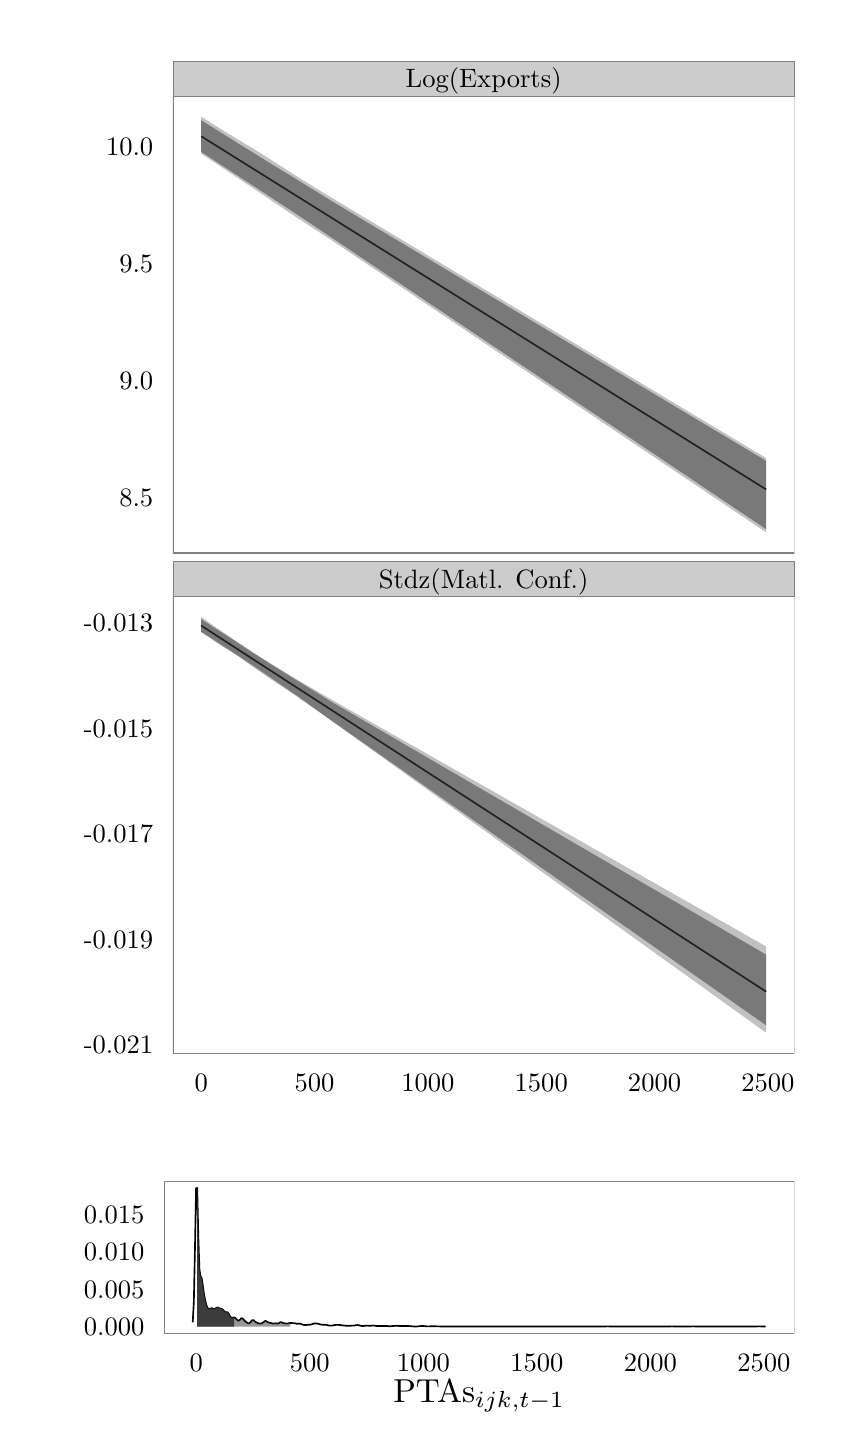
\begin{tikzpicture}[x=1pt,y=1pt]
\definecolor[named]{fillColor}{rgb}{1.00,1.00,1.00}
\path[use as bounding box,fill=fillColor,fill opacity=0.00] (0,0) rectangle (289.08,505.89);
\begin{scope}
\path[clip] (  0.00,101.18) rectangle (289.08,505.89);
\definecolor[named]{drawColor}{rgb}{1.00,1.00,1.00}
\definecolor[named]{fillColor}{rgb}{1.00,1.00,1.00}

\path[draw=drawColor,line width= 0.6pt,line join=round,line cap=round,fill=fillColor] (  0.00,101.18) rectangle (289.08,505.89);
\end{scope}
\begin{scope}
\path[clip] ( 52.48,316.03) rectangle (277.03,481.21);
\definecolor[named]{fillColor}{rgb}{1.00,1.00,1.00}

\path[fill=fillColor] ( 52.48,316.03) rectangle (277.03,481.21);
\definecolor[named]{drawColor}{rgb}{0.00,0.00,0.00}

\path[draw=drawColor,line width= 0.6pt,line join=round] ( 62.69,466.65) --
	( 62.94,466.50) --
	( 63.35,466.24) --
	( 64.08,465.78) --
	( 64.57,465.47) --
	( 65.31,465.01) --
	( 66.54,464.24) --
	( 68.26,463.17) --
	( 70.06,462.04) --
	( 71.70,461.02) --
	( 73.75,459.74) --
	( 76.53,458.00) --
	( 81.12,455.13) --
	( 88.08,450.77) --
	( 96.93,445.24) --
	(109.87,437.15) --
	(266.83,339.03);
\definecolor[named]{fillColor}{rgb}{0.20,0.20,0.20}

\path[fill=fillColor,fill opacity=0.30] ( 62.69,473.70) --
	( 62.94,473.55) --
	( 63.35,473.29) --
	( 64.08,472.84) --
	( 64.57,472.53) --
	( 65.31,472.07) --
	( 66.54,471.30) --
	( 68.26,470.23) --
	( 70.06,469.11) --
	( 71.70,468.09) --
	( 73.75,466.85) --
	( 76.53,465.17) --
	( 81.12,462.40) --
	( 88.08,458.06) --
	( 96.93,452.35) --
	(109.87,444.38) --
	(266.83,350.37) --
	(266.83,323.54) --
	(109.87,429.03) --
	( 96.93,437.47) --
	( 88.08,443.41) --
	( 81.12,448.09) --
	( 76.53,451.17) --
	( 73.75,453.04) --
	( 71.70,454.37) --
	( 70.06,455.47) --
	( 68.26,456.67) --
	( 66.54,457.82) --
	( 65.31,458.64) --
	( 64.57,459.13) --
	( 64.08,459.46) --
	( 63.35,459.95) --
	( 62.94,460.23) --
	( 62.69,460.39) --
	cycle;
\definecolor[named]{fillColor}{rgb}{0.20,0.20,0.20}

\path[fill=fillColor,fill opacity=0.50] ( 62.69,472.42) --
	( 62.94,472.27) --
	( 63.35,472.01) --
	( 64.08,471.55) --
	( 64.57,471.25) --
	( 65.31,470.79) --
	( 66.54,470.02) --
	( 68.26,468.95) --
	( 70.06,467.82) --
	( 71.70,466.80) --
	( 73.75,465.52) --
	( 76.53,463.78) --
	( 81.12,460.94) --
	( 88.08,456.62) --
	( 96.93,451.22) --
	(109.87,443.21) --
	(266.83,349.35) --
	(266.83,324.69) --
	(109.87,430.00) --
	( 96.93,438.67) --
	( 88.08,444.45) --
	( 81.12,449.01) --
	( 76.53,451.98) --
	( 73.75,453.80) --
	( 71.70,455.14) --
	( 70.06,456.20) --
	( 68.26,457.38) --
	( 66.54,458.50) --
	( 65.31,459.31) --
	( 64.57,459.80) --
	( 64.08,460.11) --
	( 63.35,460.58) --
	( 62.94,460.85) --
	( 62.69,461.01) --
	cycle;
\definecolor[named]{drawColor}{rgb}{0.50,0.50,0.50}

\path[draw=drawColor,line width= 0.6pt,line join=round,line cap=round] ( 52.48,316.03) rectangle (277.03,481.21);
\end{scope}
\begin{scope}
\path[clip] ( 52.48,135.21) rectangle (277.03,300.39);
\definecolor[named]{fillColor}{rgb}{1.00,1.00,1.00}

\path[fill=fillColor] ( 52.48,135.21) rectangle (277.03,300.39);
\definecolor[named]{drawColor}{rgb}{0.00,0.00,0.00}

\path[draw=drawColor,line width= 0.6pt,line join=round] ( 62.69,289.82) --
	( 62.94,289.67) --
	( 63.35,289.40) --
	( 64.08,288.92) --
	( 64.57,288.60) --
	( 65.31,288.13) --
	( 66.54,287.33) --
	( 68.26,286.22) --
	( 70.06,285.05) --
	( 71.70,283.99) --
	( 73.75,282.66) --
	( 76.53,280.86) --
	( 81.12,277.88) --
	( 88.08,273.37) --
	( 96.93,267.64) --
	(109.87,259.26) --
	(266.83,157.57);
\definecolor[named]{fillColor}{rgb}{0.20,0.20,0.20}

\path[fill=fillColor,fill opacity=0.30] ( 62.69,292.88) --
	( 62.94,292.73) --
	( 63.35,292.49) --
	( 64.08,291.99) --
	( 64.57,291.64) --
	( 65.31,291.11) --
	( 66.54,290.23) --
	( 68.26,289.02) --
	( 70.06,287.81) --
	( 71.70,286.70) --
	( 73.75,285.31) --
	( 76.53,283.42) --
	( 81.12,280.41) --
	( 88.08,275.97) --
	( 96.93,270.57) --
	(109.87,263.04) --
	(266.83,173.89) --
	(266.83,142.72) --
	(109.87,255.37) --
	( 96.93,264.45) --
	( 88.08,270.33) --
	( 81.12,275.14) --
	( 76.53,278.39) --
	( 73.75,280.32) --
	( 71.70,281.52) --
	( 70.06,282.45) --
	( 68.26,283.65) --
	( 66.54,284.82) --
	( 65.31,285.65) --
	( 64.57,286.15) --
	( 64.08,286.48) --
	( 63.35,286.97) --
	( 62.94,287.22) --
	( 62.69,287.36) --
	cycle;
\definecolor[named]{fillColor}{rgb}{0.20,0.20,0.20}

\path[fill=fillColor,fill opacity=0.50] ( 62.69,292.18) --
	( 62.94,292.01) --
	( 63.35,291.73) --
	( 64.08,291.25) --
	( 64.57,290.93) --
	( 65.31,290.45) --
	( 66.54,289.65) --
	( 68.26,288.54) --
	( 70.06,287.38) --
	( 71.70,286.32) --
	( 73.75,285.00) --
	( 76.53,283.19) --
	( 81.12,280.14) --
	( 88.08,275.72) --
	( 96.93,270.24) --
	(109.87,262.25) --
	(266.83,170.94) --
	(266.83,145.40) --
	(109.87,255.46) --
	( 96.93,264.75) --
	( 88.08,270.83) --
	( 81.12,275.56) --
	( 76.53,278.64) --
	( 73.75,280.40) --
	( 71.70,281.76) --
	( 70.06,282.86) --
	( 68.26,284.03) --
	( 66.54,285.14) --
	( 65.31,285.95) --
	( 64.57,286.41) --
	( 64.08,286.71) --
	( 63.35,287.18) --
	( 62.94,287.45) --
	( 62.69,287.61) --
	cycle;
\definecolor[named]{drawColor}{rgb}{0.50,0.50,0.50}

\path[draw=drawColor,line width= 0.6pt,line join=round,line cap=round] ( 52.48,135.21) rectangle (277.03,300.39);
\end{scope}
\begin{scope}
\path[clip] (  0.00,  0.00) rectangle (289.08,505.89);
\definecolor[named]{drawColor}{rgb}{0.50,0.50,0.50}
\definecolor[named]{fillColor}{rgb}{0.80,0.80,0.80}

\path[draw=drawColor,line width= 0.2pt,line join=round,line cap=round,fill=fillColor] ( 52.48,481.21) rectangle (277.03,493.84);
\definecolor[named]{drawColor}{rgb}{0.00,0.00,0.00}

\node[text=drawColor,anchor=base,inner sep=0pt, outer sep=0pt, scale=  0.96] at (164.76,484.22) {Log(Exports)};
\end{scope}
\begin{scope}
\path[clip] (  0.00,  0.00) rectangle (289.08,505.89);
\definecolor[named]{drawColor}{rgb}{0.50,0.50,0.50}
\definecolor[named]{fillColor}{rgb}{0.80,0.80,0.80}

\path[draw=drawColor,line width= 0.2pt,line join=round,line cap=round,fill=fillColor] ( 52.48,300.39) rectangle (277.03,313.02);
\definecolor[named]{drawColor}{rgb}{0.00,0.00,0.00}

\node[text=drawColor,anchor=base,inner sep=0pt, outer sep=0pt, scale=  0.96] at (164.76,303.40) {Stdz(Matl. Conf.)};
\end{scope}
\begin{scope}
\path[clip] (  0.00,  0.00) rectangle (289.08,505.89);
\definecolor[named]{drawColor}{rgb}{0.00,0.00,0.00}

\node[text=drawColor,anchor=base east,inner sep=0pt, outer sep=0pt, scale=  0.96] at ( 45.37,332.92) {8.5};

\node[text=drawColor,anchor=base east,inner sep=0pt, outer sep=0pt, scale=  0.96] at ( 45.37,375.13) {9.0};

\node[text=drawColor,anchor=base east,inner sep=0pt, outer sep=0pt, scale=  0.96] at ( 45.37,417.35) {9.5};

\node[text=drawColor,anchor=base east,inner sep=0pt, outer sep=0pt, scale=  0.96] at ( 45.37,459.56) {10.0};
\end{scope}
\begin{scope}
\path[clip] (  0.00,  0.00) rectangle (289.08,505.89);
\definecolor[named]{drawColor}{rgb}{0.00,0.00,0.00}

\node[text=drawColor,anchor=base east,inner sep=0pt, outer sep=0pt, scale=  0.96] at ( 45.37,135.03) {-0.021};

\node[text=drawColor,anchor=base east,inner sep=0pt, outer sep=0pt, scale=  0.96] at ( 45.37,173.19) {-0.019};

\node[text=drawColor,anchor=base east,inner sep=0pt, outer sep=0pt, scale=  0.96] at ( 45.37,211.34) {-0.017};

\node[text=drawColor,anchor=base east,inner sep=0pt, outer sep=0pt, scale=  0.96] at ( 45.37,249.50) {-0.015};

\node[text=drawColor,anchor=base east,inner sep=0pt, outer sep=0pt, scale=  0.96] at ( 45.37,287.65) {-0.013};
\end{scope}
\begin{scope}
\path[clip] (  0.00,  0.00) rectangle (289.08,505.89);
\definecolor[named]{drawColor}{rgb}{0.00,0.00,0.00}

\node[text=drawColor,anchor=base,inner sep=0pt, outer sep=0pt, scale=  0.96] at ( 62.69,121.49) {0};

\node[text=drawColor,anchor=base,inner sep=0pt, outer sep=0pt, scale=  0.96] at (103.65,121.49) {500};

\node[text=drawColor,anchor=base,inner sep=0pt, outer sep=0pt, scale=  0.96] at (144.61,121.49) {1000};

\node[text=drawColor,anchor=base,inner sep=0pt, outer sep=0pt, scale=  0.96] at (185.57,121.49) {1500};

\node[text=drawColor,anchor=base,inner sep=0pt, outer sep=0pt, scale=  0.96] at (226.52,121.49) {2000};

\node[text=drawColor,anchor=base,inner sep=0pt, outer sep=0pt, scale=  0.96] at (267.48,121.49) {2500};
\end{scope}
\begin{scope}
\path[clip] (  0.00,  0.00) rectangle (289.08,101.18);
\definecolor[named]{drawColor}{rgb}{1.00,1.00,1.00}
\definecolor[named]{fillColor}{rgb}{1.00,1.00,1.00}

\path[draw=drawColor,line width= 0.6pt,line join=round,line cap=round,fill=fillColor] ( -0.00,  0.00) rectangle (289.08,101.18);
\end{scope}
\begin{scope}
\path[clip] ( 49.28, 34.03) rectangle (277.04, 89.13);
\definecolor[named]{fillColor}{rgb}{1.00,1.00,1.00}

\path[fill=fillColor] ( 49.28, 34.03) rectangle (277.04, 89.13);
\definecolor[named]{drawColor}{rgb}{0.00,0.00,0.00}

\path[draw=drawColor,line width= 0.6pt,line join=round] ( 59.64, 38.05) --
	( 60.04, 45.39) --
	( 60.45, 64.85) --
	( 60.85, 86.49) --
	( 61.26, 86.63) --
	( 61.66, 69.17) --
	( 62.07, 57.11) --
	( 62.47, 54.76) --
	( 62.88, 53.97) --
	( 63.28, 51.42) --
	( 63.69, 48.50) --
	( 64.09, 46.23) --
	( 64.50, 44.54) --
	( 64.90, 43.44) --
	( 65.31, 43.00) --
	( 65.71, 42.85) --
	( 66.12, 43.03) --
	( 66.52, 43.25) --
	( 66.93, 42.98) --
	( 67.33, 42.78) --
	( 67.74, 42.97) --
	( 68.15, 43.27) --
	( 68.55, 43.45) --
	( 68.96, 43.34) --
	( 69.36, 43.10) --
	( 69.77, 42.99) --
	( 70.17, 42.90) --
	( 70.58, 42.58) --
	( 70.98, 42.09) --
	( 71.39, 41.76) --
	( 71.79, 41.75) --
	( 72.20, 41.71) --
	( 72.60, 41.19) --
	( 73.01, 40.38) --
	( 73.41, 39.86) --
	( 73.82, 39.74) --
	( 74.22, 39.79) --
	( 74.63, 39.79) --
	( 75.03, 39.62) --
	( 75.44, 39.22) --
	( 75.84, 38.78) --
	( 76.25, 38.63) --
	( 76.65, 38.91) --
	( 77.06, 39.40) --
	( 77.46, 39.57) --
	( 77.87, 39.24) --
	( 78.27, 38.74) --
	( 78.68, 38.34) --
	( 79.09, 38.05) --
	( 79.49, 37.81) --
	( 79.90, 37.72) --
	( 80.30, 37.87) --
	( 80.71, 38.33) --
	( 81.11, 38.84) --
	( 81.52, 38.88) --
	( 81.92, 38.51) --
	( 82.33, 38.20) --
	( 82.73, 37.99) --
	( 83.14, 37.79) --
	( 83.54, 37.66) --
	( 83.95, 37.62) --
	( 84.35, 37.65) --
	( 84.76, 37.79) --
	( 85.16, 38.04) --
	( 85.57, 38.41) --
	( 85.97, 38.60) --
	( 86.38, 38.39) --
	( 86.78, 38.11) --
	( 87.19, 37.98) --
	( 87.59, 37.88) --
	( 88.00, 37.77) --
	( 88.40, 37.67) --
	( 88.81, 37.64) --
	( 89.21, 37.69) --
	( 89.62, 37.71) --
	( 90.02, 37.64) --
	( 90.43, 37.64) --
	( 90.84, 37.81) --
	( 91.24, 38.06) --
	( 91.65, 38.11) --
	( 92.05, 37.92) --
	( 92.46, 37.76) --
	( 92.86, 37.72) --
	( 93.27, 37.65) --
	( 93.67, 37.58) --
	( 94.08, 37.64) --
	( 94.48, 37.78) --
	( 94.89, 37.84) --
	( 95.29, 37.80) --
	( 95.70, 37.78) --
	( 96.10, 37.79) --
	( 96.51, 37.75) --
	( 96.91, 37.64) --
	( 97.32, 37.53) --
	( 97.72, 37.54) --
	( 98.13, 37.61) --
	( 98.53, 37.56) --
	( 98.94, 37.39) --
	( 99.34, 37.23) --
	( 99.75, 37.13) --
	(100.15, 37.11) --
	(100.56, 37.11) --
	(100.96, 37.14) --
	(101.37, 37.17) --
	(101.78, 37.19) --
	(102.18, 37.23) --
	(102.59, 37.33) --
	(102.99, 37.49) --
	(103.40, 37.62) --
	(103.80, 37.65) --
	(104.21, 37.62) --
	(104.61, 37.61) --
	(105.02, 37.53) --
	(105.42, 37.39) --
	(105.83, 37.28) --
	(106.23, 37.23) --
	(106.64, 37.20) --
	(107.04, 37.20) --
	(107.45, 37.21) --
	(107.85, 37.16) --
	(108.26, 37.05) --
	(108.66, 36.93) --
	(109.07, 36.88) --
	(109.47, 36.87) --
	(109.88, 36.89) --
	(110.28, 36.96) --
	(110.69, 37.05) --
	(111.09, 37.11) --
	(111.50, 37.13) --
	(111.90, 37.13) --
	(112.31, 37.13) --
	(112.71, 37.12) --
	(113.12, 37.08) --
	(113.53, 36.99) --
	(113.93, 36.93) --
	(114.34, 36.91) --
	(114.74, 36.86) --
	(115.15, 36.82) --
	(115.55, 36.82) --
	(115.96, 36.85) --
	(116.36, 36.85) --
	(116.77, 36.85) --
	(117.17, 36.86) --
	(117.58, 36.88) --
	(117.98, 36.91) --
	(118.39, 36.99) --
	(118.79, 37.06) --
	(119.20, 37.08) --
	(119.60, 37.03) --
	(120.01, 36.93) --
	(120.41, 36.82) --
	(120.82, 36.75) --
	(121.22, 36.75) --
	(121.63, 36.79) --
	(122.03, 36.84) --
	(122.44, 36.86) --
	(122.84, 36.87) --
	(123.25, 36.85) --
	(123.65, 36.82) --
	(124.06, 36.83) --
	(124.47, 36.88) --
	(124.87, 36.90) --
	(125.28, 36.87) --
	(125.68, 36.80) --
	(126.09, 36.74) --
	(126.49, 36.72) --
	(126.90, 36.72) --
	(127.30, 36.71) --
	(127.71, 36.71) --
	(128.11, 36.72) --
	(128.52, 36.74) --
	(128.92, 36.76) --
	(129.33, 36.76) --
	(129.73, 36.75) --
	(130.14, 36.71) --
	(130.54, 36.67) --
	(130.95, 36.65) --
	(131.35, 36.68) --
	(131.76, 36.73) --
	(132.16, 36.76) --
	(132.57, 36.77) --
	(132.97, 36.80) --
	(133.38, 36.81) --
	(133.78, 36.78) --
	(134.19, 36.76) --
	(134.59, 36.74) --
	(135.00, 36.73) --
	(135.40, 36.73) --
	(135.81, 36.73) --
	(136.22, 36.72) --
	(136.62, 36.73) --
	(137.03, 36.75) --
	(137.43, 36.73) --
	(137.84, 36.71) --
	(138.24, 36.69) --
	(138.65, 36.64) --
	(139.05, 36.60) --
	(139.46, 36.58) --
	(139.86, 36.57) --
	(140.27, 36.57) --
	(140.67, 36.59) --
	(141.08, 36.61) --
	(141.48, 36.65) --
	(141.89, 36.71) --
	(142.29, 36.74) --
	(142.70, 36.73) --
	(143.10, 36.72) --
	(143.51, 36.69) --
	(143.91, 36.64) --
	(144.32, 36.60) --
	(144.72, 36.60) --
	(145.13, 36.61) --
	(145.53, 36.63) --
	(145.94, 36.64) --
	(146.34, 36.64) --
	(146.75, 36.64) --
	(147.16, 36.64) --
	(147.56, 36.62) --
	(147.97, 36.61) --
	(148.37, 36.60) --
	(148.78, 36.59) --
	(149.18, 36.57) --
	(149.59, 36.57) --
	(149.99, 36.57) --
	(150.40, 36.58) --
	(150.80, 36.58) --
	(151.21, 36.57) --
	(151.61, 36.57) --
	(152.02, 36.57) --
	(152.42, 36.56) --
	(152.83, 36.55) --
	(153.23, 36.54) --
	(153.64, 36.54) --
	(154.04, 36.54) --
	(154.45, 36.54) --
	(154.85, 36.54) --
	(155.26, 36.54) --
	(155.66, 36.54) --
	(156.07, 36.54) --
	(156.47, 36.54) --
	(156.88, 36.54) --
	(157.28, 36.54) --
	(157.69, 36.54) --
	(158.09, 36.54) --
	(158.50, 36.54) --
	(158.91, 36.54) --
	(159.31, 36.54) --
	(159.72, 36.54) --
	(160.12, 36.54) --
	(160.53, 36.54) --
	(160.93, 36.54) --
	(161.34, 36.54) --
	(161.74, 36.54) --
	(162.15, 36.55) --
	(162.55, 36.56) --
	(162.96, 36.56) --
	(163.36, 36.57) --
	(163.77, 36.56) --
	(164.17, 36.56) --
	(164.58, 36.55) --
	(164.98, 36.55) --
	(165.39, 36.54) --
	(165.79, 36.54) --
	(166.20, 36.55) --
	(166.60, 36.56) --
	(167.01, 36.58) --
	(167.41, 36.58) --
	(167.82, 36.58) --
	(168.22, 36.57) --
	(168.63, 36.56) --
	(169.03, 36.56) --
	(169.44, 36.55) --
	(169.85, 36.55) --
	(170.25, 36.55) --
	(170.66, 36.55) --
	(171.06, 36.55) --
	(171.47, 36.55) --
	(171.87, 36.55) --
	(172.28, 36.54) --
	(172.68, 36.54) --
	(173.09, 36.54) --
	(173.49, 36.54) --
	(173.90, 36.54) --
	(174.30, 36.54) --
	(174.71, 36.54) --
	(175.11, 36.54) --
	(175.52, 36.54) --
	(175.92, 36.54) --
	(176.33, 36.54) --
	(176.73, 36.54) --
	(177.14, 36.54) --
	(177.54, 36.54) --
	(177.95, 36.54) --
	(178.35, 36.54) --
	(178.76, 36.54) --
	(179.16, 36.54) --
	(179.57, 36.54) --
	(179.97, 36.54) --
	(180.38, 36.54) --
	(180.78, 36.54) --
	(181.19, 36.54) --
	(181.60, 36.54) --
	(182.00, 36.54) --
	(182.41, 36.54) --
	(182.81, 36.54) --
	(183.22, 36.54) --
	(183.62, 36.54) --
	(184.03, 36.54) --
	(184.43, 36.54) --
	(184.84, 36.54) --
	(185.24, 36.55) --
	(185.65, 36.55) --
	(186.05, 36.55) --
	(186.46, 36.54) --
	(186.86, 36.54) --
	(187.27, 36.54) --
	(187.67, 36.55) --
	(188.08, 36.55) --
	(188.48, 36.55) --
	(188.89, 36.56) --
	(189.29, 36.56) --
	(189.70, 36.56) --
	(190.10, 36.56) --
	(190.51, 36.55) --
	(190.91, 36.55) --
	(191.32, 36.54) --
	(191.72, 36.54) --
	(192.13, 36.54) --
	(192.54, 36.54) --
	(192.94, 36.54) --
	(193.35, 36.54) --
	(193.75, 36.54) --
	(194.16, 36.54) --
	(194.56, 36.54) --
	(194.97, 36.54) --
	(195.37, 36.54) --
	(195.78, 36.54) --
	(196.18, 36.54) --
	(196.59, 36.54) --
	(196.99, 36.54) --
	(197.40, 36.54) --
	(197.80, 36.54) --
	(198.21, 36.54) --
	(198.61, 36.54) --
	(199.02, 36.54) --
	(199.42, 36.54) --
	(199.83, 36.54) --
	(200.23, 36.54) --
	(200.64, 36.54) --
	(201.04, 36.54) --
	(201.45, 36.54) --
	(201.85, 36.54) --
	(202.26, 36.54) --
	(202.66, 36.54) --
	(203.07, 36.54) --
	(203.47, 36.54) --
	(203.88, 36.54) --
	(204.29, 36.54) --
	(204.69, 36.54) --
	(205.10, 36.54) --
	(205.50, 36.54) --
	(205.91, 36.54) --
	(206.31, 36.55) --
	(206.72, 36.56) --
	(207.12, 36.57) --
	(207.53, 36.58) --
	(207.93, 36.57) --
	(208.34, 36.57) --
	(208.74, 36.57) --
	(209.15, 36.59) --
	(209.55, 36.60) --
	(209.96, 36.59) --
	(210.36, 36.57) --
	(210.77, 36.55) --
	(211.17, 36.54) --
	(211.58, 36.54) --
	(211.98, 36.54) --
	(212.39, 36.54) --
	(212.79, 36.54) --
	(213.20, 36.54) --
	(213.60, 36.54) --
	(214.01, 36.54) --
	(214.41, 36.54) --
	(214.82, 36.54) --
	(215.23, 36.54) --
	(215.63, 36.54) --
	(216.04, 36.54) --
	(216.44, 36.54) --
	(216.85, 36.54) --
	(217.25, 36.54) --
	(217.66, 36.54) --
	(218.06, 36.54) --
	(218.47, 36.54) --
	(218.87, 36.54) --
	(219.28, 36.54) --
	(219.68, 36.54) --
	(220.09, 36.54) --
	(220.49, 36.54) --
	(220.90, 36.54) --
	(221.30, 36.54) --
	(221.71, 36.54) --
	(222.11, 36.54) --
	(222.52, 36.54) --
	(222.92, 36.54) --
	(223.33, 36.54) --
	(223.73, 36.54) --
	(224.14, 36.54) --
	(224.54, 36.55) --
	(224.95, 36.55) --
	(225.35, 36.55) --
	(225.76, 36.54) --
	(226.16, 36.54) --
	(226.57, 36.54) --
	(226.98, 36.54) --
	(227.38, 36.54) --
	(227.79, 36.54) --
	(228.19, 36.54) --
	(228.60, 36.54) --
	(229.00, 36.54) --
	(229.41, 36.55) --
	(229.81, 36.56) --
	(230.22, 36.57) --
	(230.62, 36.57) --
	(231.03, 36.56) --
	(231.43, 36.56) --
	(231.84, 36.57) --
	(232.24, 36.58) --
	(232.65, 36.59) --
	(233.05, 36.59) --
	(233.46, 36.58) --
	(233.86, 36.56) --
	(234.27, 36.55) --
	(234.67, 36.54) --
	(235.08, 36.54) --
	(235.48, 36.54) --
	(235.89, 36.54) --
	(236.29, 36.54) --
	(236.70, 36.54) --
	(237.10, 36.54) --
	(237.51, 36.54) --
	(237.92, 36.54) --
	(238.32, 36.54) --
	(238.73, 36.55) --
	(239.13, 36.56) --
	(239.54, 36.57) --
	(239.94, 36.59) --
	(240.35, 36.61) --
	(240.75, 36.60) --
	(241.16, 36.57) --
	(241.56, 36.55) --
	(241.97, 36.54) --
	(242.37, 36.54) --
	(242.78, 36.54) --
	(243.18, 36.54) --
	(243.59, 36.54) --
	(243.99, 36.54) --
	(244.40, 36.54) --
	(244.80, 36.54) --
	(245.21, 36.54) --
	(245.61, 36.54) --
	(246.02, 36.54) --
	(246.42, 36.54) --
	(246.83, 36.54) --
	(247.23, 36.54) --
	(247.64, 36.54) --
	(248.04, 36.54) --
	(248.45, 36.54) --
	(248.85, 36.54) --
	(249.26, 36.54) --
	(249.67, 36.54) --
	(250.07, 36.54) --
	(250.48, 36.54) --
	(250.88, 36.54) --
	(251.29, 36.54) --
	(251.69, 36.54) --
	(252.10, 36.54) --
	(252.50, 36.54) --
	(252.91, 36.54) --
	(253.31, 36.54) --
	(253.72, 36.54) --
	(254.12, 36.54) --
	(254.53, 36.54) --
	(254.93, 36.54) --
	(255.34, 36.54) --
	(255.74, 36.55) --
	(256.15, 36.55) --
	(256.55, 36.55) --
	(256.96, 36.55) --
	(257.36, 36.54) --
	(257.77, 36.54) --
	(258.17, 36.54) --
	(258.58, 36.54) --
	(258.98, 36.54) --
	(259.39, 36.54) --
	(259.79, 36.54) --
	(260.20, 36.54) --
	(260.61, 36.54) --
	(261.01, 36.54) --
	(261.42, 36.54) --
	(261.82, 36.54) --
	(262.23, 36.54) --
	(262.63, 36.55) --
	(263.04, 36.56) --
	(263.44, 36.57) --
	(263.85, 36.60) --
	(264.25, 36.61) --
	(264.66, 36.60) --
	(265.06, 36.58) --
	(265.47, 36.56) --
	(265.87, 36.55) --
	(266.28, 36.54) --
	(266.68, 36.54);
\definecolor[named]{fillColor}{rgb}{0.20,0.20,0.20}

\path[fill=fillColor,fill opacity=0.50] ( 61.26, 86.63) --
	( 61.66, 69.17) --
	( 62.07, 57.11) --
	( 62.47, 54.76) --
	( 62.88, 53.97) --
	( 63.28, 51.42) --
	( 63.69, 48.50) --
	( 64.09, 46.23) --
	( 64.50, 44.54) --
	( 64.90, 43.44) --
	( 65.31, 43.00) --
	( 65.71, 42.85) --
	( 66.12, 43.03) --
	( 66.52, 43.25) --
	( 66.93, 42.98) --
	( 67.33, 42.78) --
	( 67.74, 42.97) --
	( 68.15, 43.27) --
	( 68.55, 43.45) --
	( 68.96, 43.34) --
	( 69.36, 43.10) --
	( 69.77, 42.99) --
	( 70.17, 42.90) --
	( 70.58, 42.58) --
	( 70.98, 42.09) --
	( 71.39, 41.76) --
	( 71.79, 41.75) --
	( 72.20, 41.71) --
	( 72.60, 41.19) --
	( 73.01, 40.38) --
	( 73.41, 39.86) --
	( 73.82, 39.74) --
	( 74.22, 39.79) --
	( 74.63, 39.79) --
	( 75.03, 39.62) --
	( 75.44, 39.22) --
	( 75.84, 38.78) --
	( 76.25, 38.63) --
	( 76.65, 38.91) --
	( 77.06, 39.40) --
	( 77.46, 39.57) --
	( 77.87, 39.24) --
	( 78.27, 38.74) --
	( 78.68, 38.34) --
	( 79.09, 38.05) --
	( 79.49, 37.81) --
	( 79.90, 37.72) --
	( 80.30, 37.87) --
	( 80.71, 38.33) --
	( 81.11, 38.84) --
	( 81.52, 38.88) --
	( 81.92, 38.51) --
	( 82.33, 38.20) --
	( 82.73, 37.99) --
	( 83.14, 37.79) --
	( 83.54, 37.66) --
	( 83.95, 37.62) --
	( 84.35, 37.65) --
	( 84.76, 37.79) --
	( 85.16, 38.04) --
	( 85.57, 38.41) --
	( 85.97, 38.60) --
	( 86.38, 38.39) --
	( 86.78, 38.11) --
	( 87.19, 37.98) --
	( 87.59, 37.88) --
	( 88.00, 37.77) --
	( 88.40, 37.67) --
	( 88.81, 37.64) --
	( 89.21, 37.69) --
	( 89.62, 37.71) --
	( 90.02, 37.64) --
	( 90.43, 37.64) --
	( 90.84, 37.81) --
	( 91.24, 38.06) --
	( 91.65, 38.11) --
	( 92.05, 37.92) --
	( 92.46, 37.76) --
	( 92.86, 37.72) --
	( 93.27, 37.65) --
	( 93.67, 37.58) --
	( 94.08, 37.64) --
	( 94.48, 37.78) --
	( 94.89, 37.84) --
	( 94.89, 36.54) --
	( 94.48, 36.54) --
	( 94.08, 36.54) --
	( 93.67, 36.54) --
	( 93.27, 36.54) --
	( 92.86, 36.54) --
	( 92.46, 36.54) --
	( 92.05, 36.54) --
	( 91.65, 36.54) --
	( 91.24, 36.54) --
	( 90.84, 36.54) --
	( 90.43, 36.54) --
	( 90.02, 36.54) --
	( 89.62, 36.54) --
	( 89.21, 36.54) --
	( 88.81, 36.54) --
	( 88.40, 36.54) --
	( 88.00, 36.54) --
	( 87.59, 36.54) --
	( 87.19, 36.54) --
	( 86.78, 36.54) --
	( 86.38, 36.54) --
	( 85.97, 36.54) --
	( 85.57, 36.54) --
	( 85.16, 36.54) --
	( 84.76, 36.54) --
	( 84.35, 36.54) --
	( 83.95, 36.54) --
	( 83.54, 36.54) --
	( 83.14, 36.54) --
	( 82.73, 36.54) --
	( 82.33, 36.54) --
	( 81.92, 36.54) --
	( 81.52, 36.54) --
	( 81.11, 36.54) --
	( 80.71, 36.54) --
	( 80.30, 36.54) --
	( 79.90, 36.54) --
	( 79.49, 36.54) --
	( 79.09, 36.54) --
	( 78.68, 36.54) --
	( 78.27, 36.54) --
	( 77.87, 36.54) --
	( 77.46, 36.54) --
	( 77.06, 36.54) --
	( 76.65, 36.54) --
	( 76.25, 36.54) --
	( 75.84, 36.54) --
	( 75.44, 36.54) --
	( 75.03, 36.54) --
	( 74.63, 36.54) --
	( 74.22, 36.54) --
	( 73.82, 36.54) --
	( 73.41, 36.54) --
	( 73.01, 36.54) --
	( 72.60, 36.54) --
	( 72.20, 36.54) --
	( 71.79, 36.54) --
	( 71.39, 36.54) --
	( 70.98, 36.54) --
	( 70.58, 36.54) --
	( 70.17, 36.54) --
	( 69.77, 36.54) --
	( 69.36, 36.54) --
	( 68.96, 36.54) --
	( 68.55, 36.54) --
	( 68.15, 36.54) --
	( 67.74, 36.54) --
	( 67.33, 36.54) --
	( 66.93, 36.54) --
	( 66.52, 36.54) --
	( 66.12, 36.54) --
	( 65.71, 36.54) --
	( 65.31, 36.54) --
	( 64.90, 36.54) --
	( 64.50, 36.54) --
	( 64.09, 36.54) --
	( 63.69, 36.54) --
	( 63.28, 36.54) --
	( 62.88, 36.54) --
	( 62.47, 36.54) --
	( 62.07, 36.54) --
	( 61.66, 36.54) --
	( 61.26, 36.54) --
	cycle;
\definecolor[named]{fillColor}{rgb}{0.20,0.20,0.20}

\path[fill=fillColor,fill opacity=0.90] ( 61.26, 86.63) --
	( 61.66, 69.17) --
	( 62.07, 57.11) --
	( 62.47, 54.76) --
	( 62.88, 53.97) --
	( 63.28, 51.42) --
	( 63.69, 48.50) --
	( 64.09, 46.23) --
	( 64.50, 44.54) --
	( 64.90, 43.44) --
	( 65.31, 43.00) --
	( 65.71, 42.85) --
	( 66.12, 43.03) --
	( 66.52, 43.25) --
	( 66.93, 42.98) --
	( 67.33, 42.78) --
	( 67.74, 42.97) --
	( 68.15, 43.27) --
	( 68.55, 43.45) --
	( 68.96, 43.34) --
	( 69.36, 43.10) --
	( 69.77, 42.99) --
	( 70.17, 42.90) --
	( 70.58, 42.58) --
	( 70.98, 42.09) --
	( 71.39, 41.76) --
	( 71.79, 41.75) --
	( 72.20, 41.71) --
	( 72.60, 41.19) --
	( 73.01, 40.38) --
	( 73.41, 39.86) --
	( 73.82, 39.74) --
	( 74.22, 39.79) --
	( 74.63, 39.79) --
	( 74.63, 36.54) --
	( 74.22, 36.54) --
	( 73.82, 36.54) --
	( 73.41, 36.54) --
	( 73.01, 36.54) --
	( 72.60, 36.54) --
	( 72.20, 36.54) --
	( 71.79, 36.54) --
	( 71.39, 36.54) --
	( 70.98, 36.54) --
	( 70.58, 36.54) --
	( 70.17, 36.54) --
	( 69.77, 36.54) --
	( 69.36, 36.54) --
	( 68.96, 36.54) --
	( 68.55, 36.54) --
	( 68.15, 36.54) --
	( 67.74, 36.54) --
	( 67.33, 36.54) --
	( 66.93, 36.54) --
	( 66.52, 36.54) --
	( 66.12, 36.54) --
	( 65.71, 36.54) --
	( 65.31, 36.54) --
	( 64.90, 36.54) --
	( 64.50, 36.54) --
	( 64.09, 36.54) --
	( 63.69, 36.54) --
	( 63.28, 36.54) --
	( 62.88, 36.54) --
	( 62.47, 36.54) --
	( 62.07, 36.54) --
	( 61.66, 36.54) --
	( 61.26, 36.54) --
	cycle;
\definecolor[named]{drawColor}{rgb}{0.50,0.50,0.50}

\path[draw=drawColor,line width= 0.6pt,line join=round,line cap=round] ( 49.28, 34.03) rectangle (277.04, 89.13);
\end{scope}
\begin{scope}
\path[clip] (  0.00,  0.00) rectangle (289.08,505.89);
\definecolor[named]{drawColor}{rgb}{0.00,0.00,0.00}

\node[text=drawColor,anchor=base east,inner sep=0pt, outer sep=0pt, scale=  0.96] at ( 42.17, 33.23) {0.000};

\node[text=drawColor,anchor=base east,inner sep=0pt, outer sep=0pt, scale=  0.96] at ( 42.17, 46.79) {0.005};

\node[text=drawColor,anchor=base east,inner sep=0pt, outer sep=0pt, scale=  0.96] at ( 42.17, 60.35) {0.010};

\node[text=drawColor,anchor=base east,inner sep=0pt, outer sep=0pt, scale=  0.96] at ( 42.17, 73.92) {0.015};
\end{scope}
\begin{scope}
\path[clip] (  0.00,  0.00) rectangle (289.08,505.89);
\definecolor[named]{drawColor}{rgb}{0.00,0.00,0.00}

\node[text=drawColor,anchor=base,inner sep=0pt, outer sep=0pt, scale=  0.96] at ( 60.93, 20.31) {0};

\node[text=drawColor,anchor=base,inner sep=0pt, outer sep=0pt, scale=  0.96] at (101.95, 20.31) {500};

\node[text=drawColor,anchor=base,inner sep=0pt, outer sep=0pt, scale=  0.96] at (142.98, 20.31) {1000};

\node[text=drawColor,anchor=base,inner sep=0pt, outer sep=0pt, scale=  0.96] at (184.00, 20.31) {1500};

\node[text=drawColor,anchor=base,inner sep=0pt, outer sep=0pt, scale=  0.96] at (225.02, 20.31) {2000};

\node[text=drawColor,anchor=base,inner sep=0pt, outer sep=0pt, scale=  0.96] at (266.04, 20.31) {2500};
\end{scope}
\begin{scope}
\path[clip] (  0.00,  0.00) rectangle (289.08,505.89);
\definecolor[named]{drawColor}{rgb}{0.00,0.00,0.00}

\node[text=drawColor,anchor=base,inner sep=0pt, outer sep=0pt, scale=  1.20] at (163.16,  9.03) {PTAs$_{ijk, t-1}$};
\end{scope}
\end{tikzpicture}
}  
    \end{tabular}
  \end{figure}
}
%%%%%%%%%%%%%%%%%%%%%%%%%%%%%%%%%%%%%%%%%%%%%%%%%%%%%%%%%%%%

%%%%%%%%%%%%%%%%%%%%%%%%%%%%%%%%%%%%%%%%%%%%%%%%%%%%%%%%%%%%
\frame
{
\frametitle{Aggregate Performance \& RMSE by i-j}
  % latex table generated in R 3.1.2 by xtable 1.7-4 package
% Mon Jun 29 06:43:03 2015
\begin{table}[ht]
\centering
\begin{tabular}{rrr}
  \hline
 & RMSE & R$^{2}$ \\ 
  \hline
Log(Exports) & 2.32 & 0.95 \\ 
  Std(Matl. Conf.) & 0.85 & 0.28 \\ 
   \hline
\end{tabular}
\end{table}

  \begin{figure}[ht]
  \centering
    \begin{tabular}{cc}
    \hspace*{-.63in}
      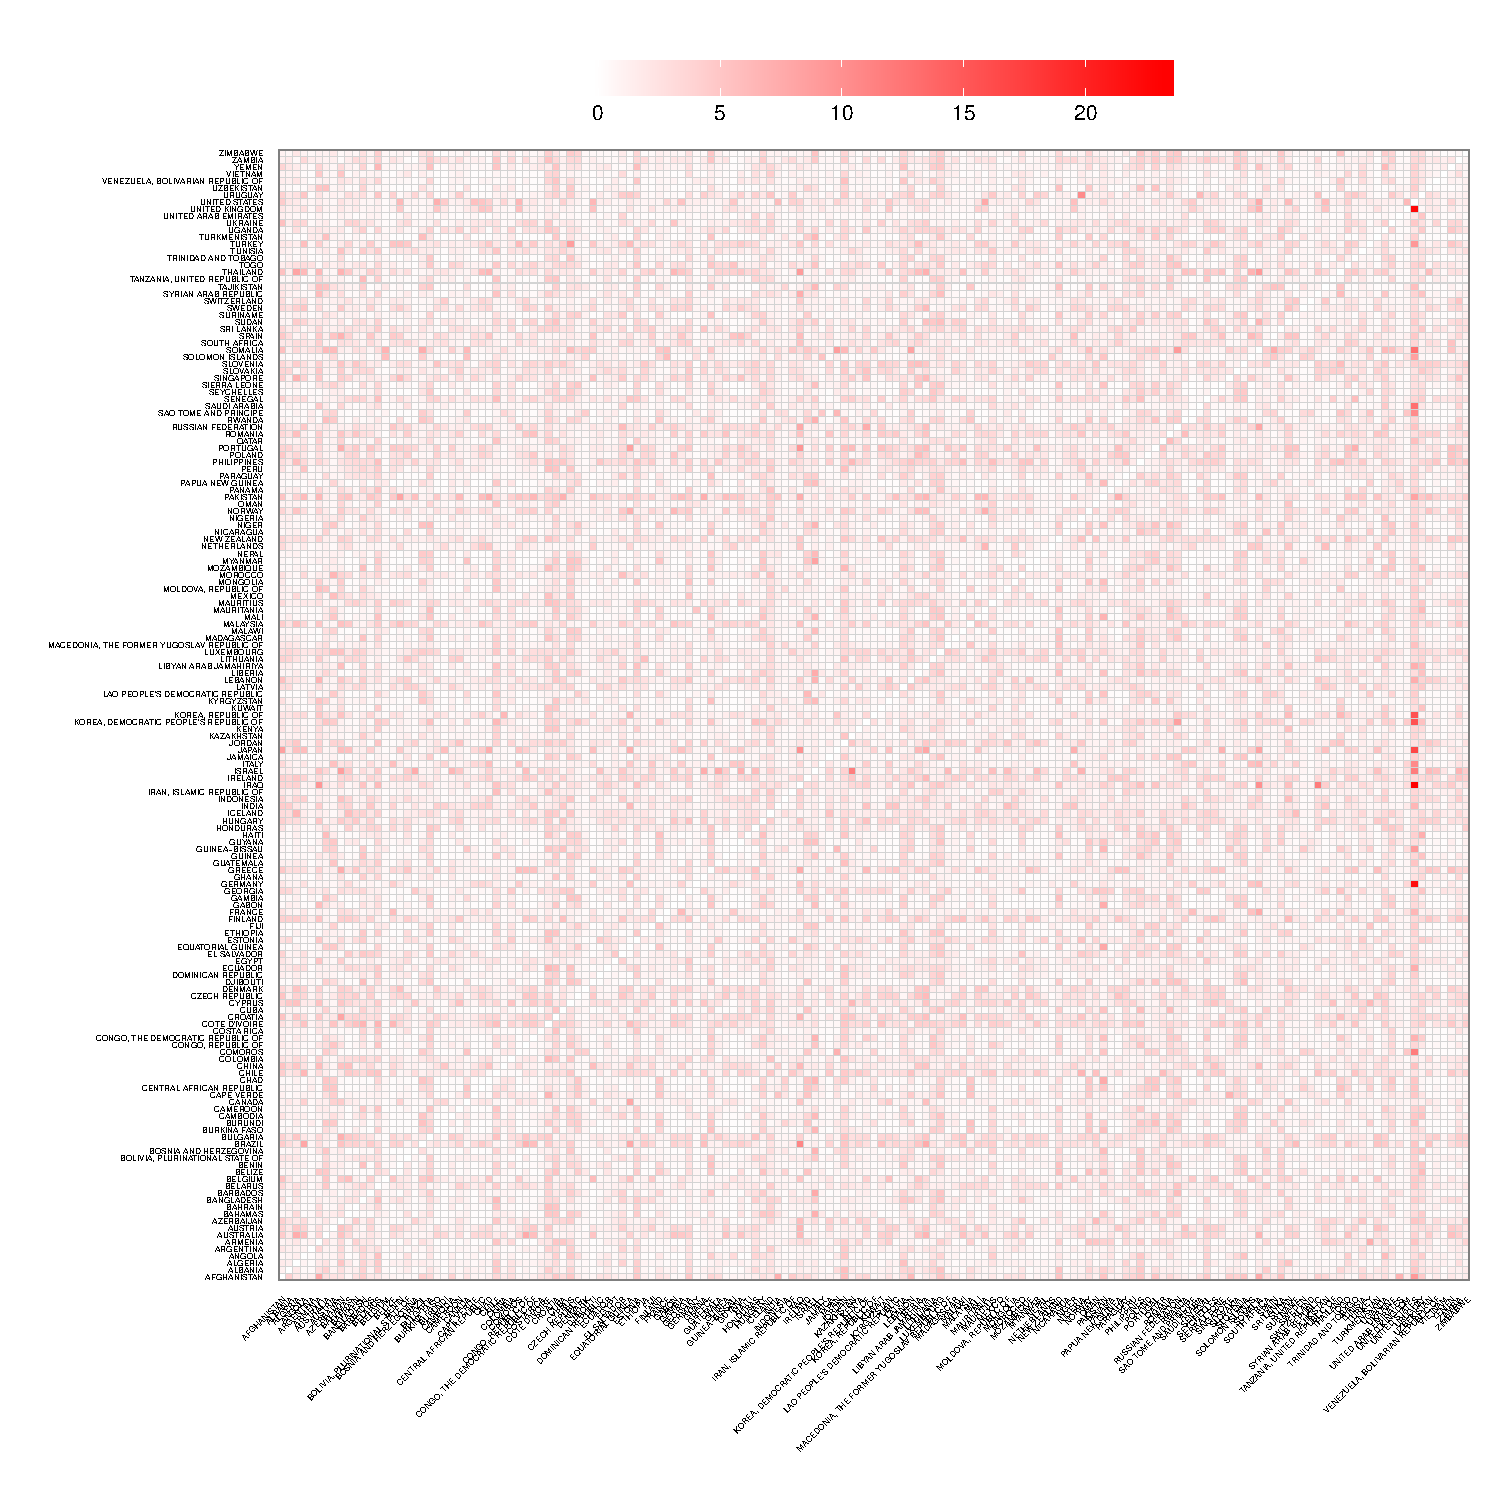
\includegraphics[width=.6\textwidth]{expiperf.pdf} & 
      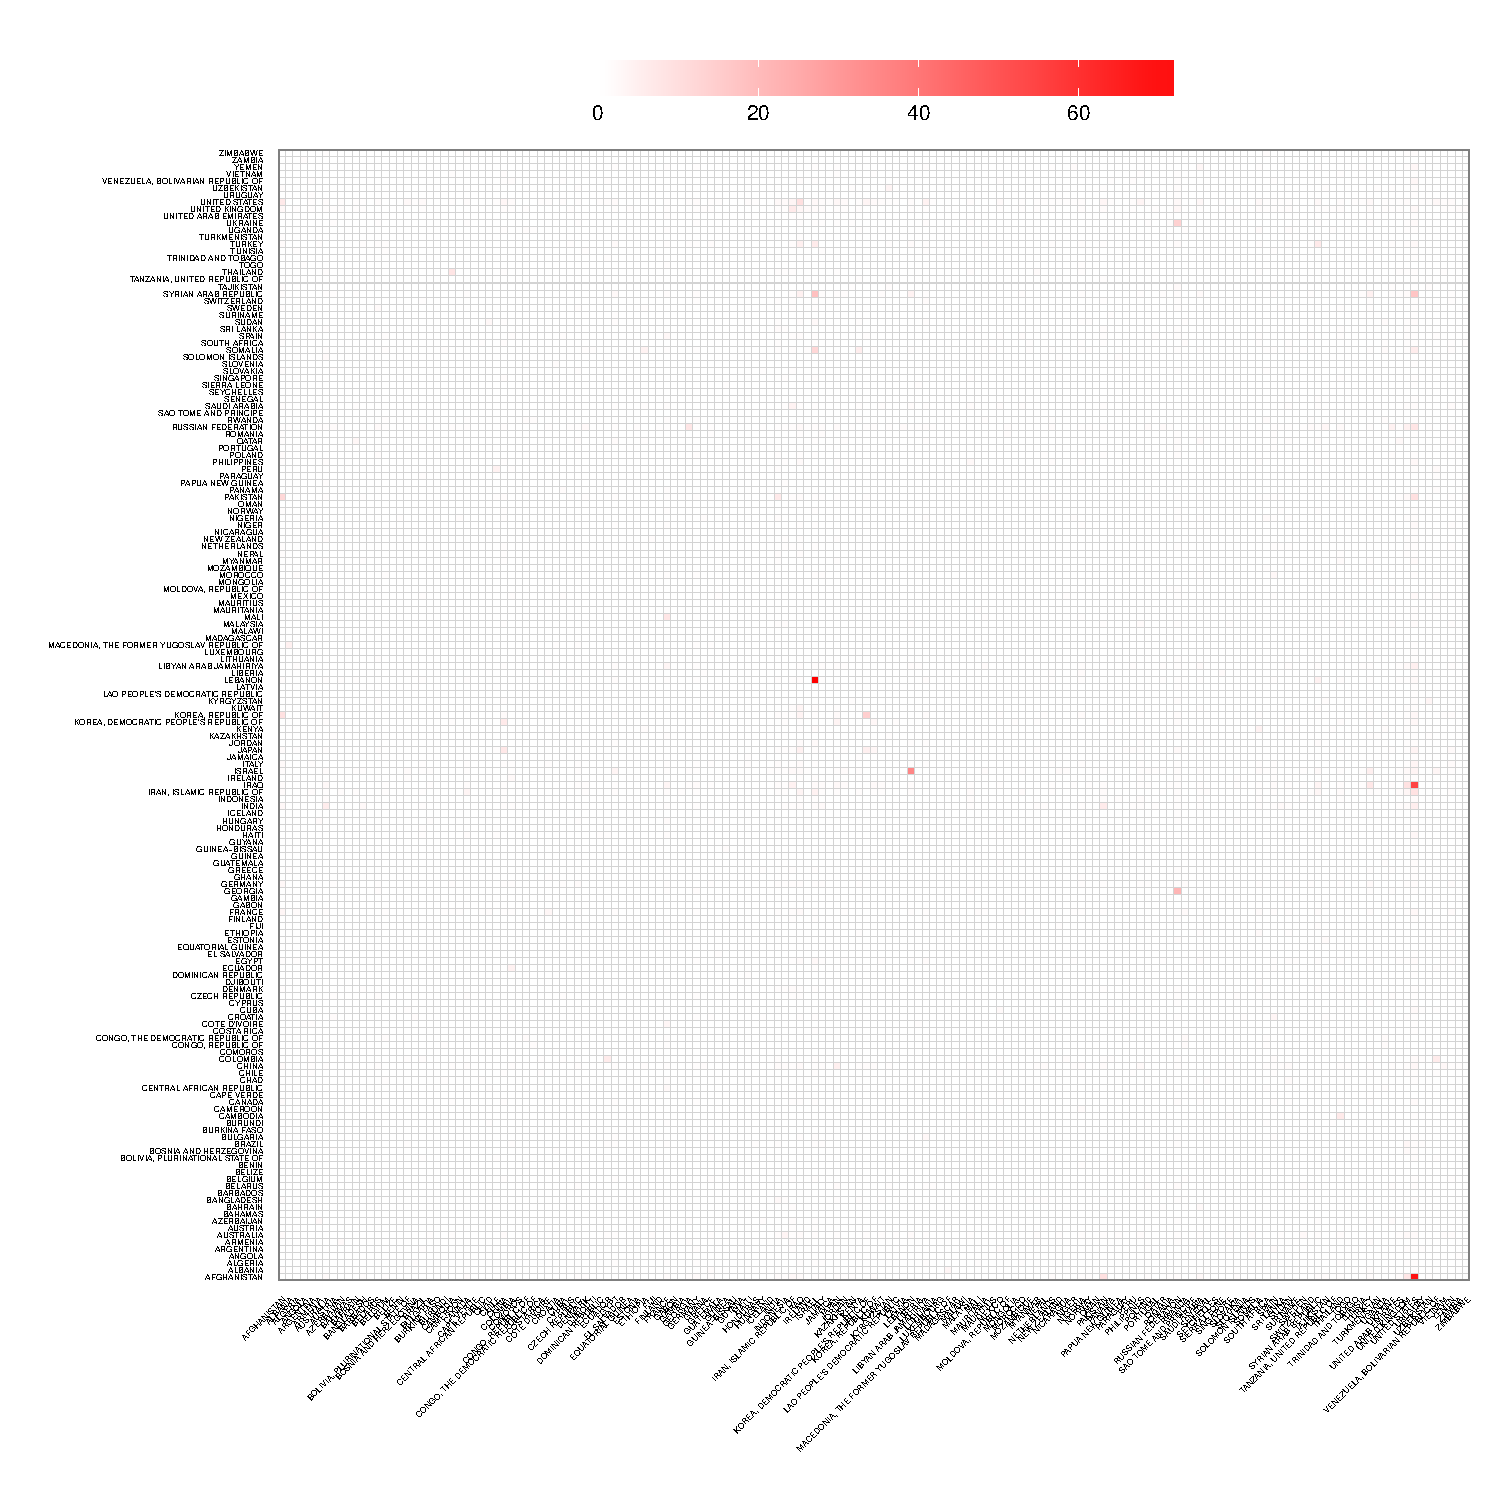
\includegraphics[width=.6\textwidth]{mconfiperf.pdf}
    \end{tabular}
  \end{figure}
}
%%%%%%%%%%%%%%%%%%%%%%%%%%%%%%%%%%%%%%%%%%%%%%%%%%%%%%%%%%%%

%%%%%%%%%%%%%%%%%%%%%%%%%%%%%%%%%%%%%%%%%%%%%%%%%%%%%%%%%%%%
\frame
{
\frametitle{Trace Plots for $\boldsymbol{\beta_{3}}$}
  \centering
  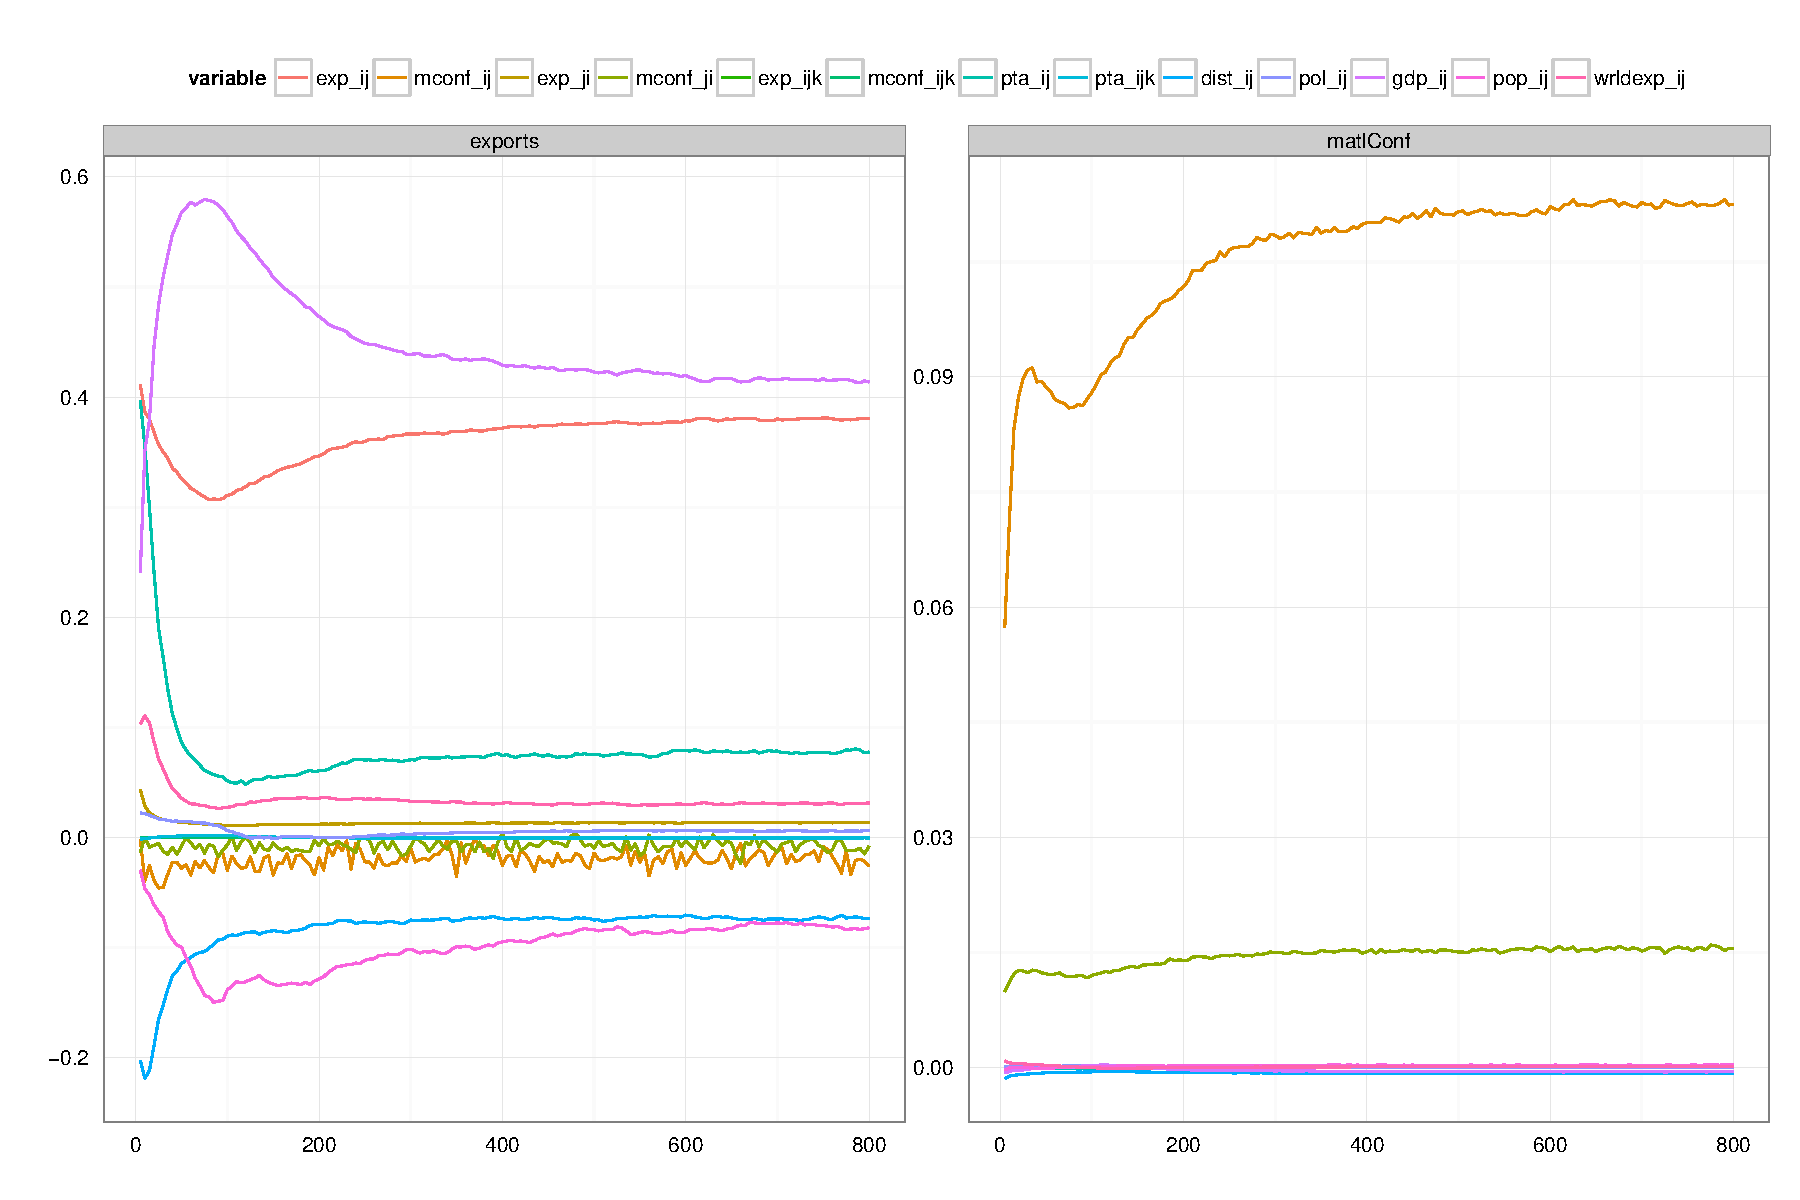
\includegraphics[width=1\textwidth]{trace.pdf}
}
%%%%%%%%%%%%%%%%%%%%%%%%%%%%%%%%%%%%%%%%%%%%%%%%%%%%%%%%%%%%

%%%%%%%%%%%%%%%%%%%%%%%%%%%%%%%%%%%%%%%%%%%%%%%%%%%%%%%%%%%%
\frame
{
  \frametitle{Comparison with directed dyadic model}
  \begin{itemize}
  \item Here I run a similar analysis using the standard directed dyadic (dd) framework
  \item The covariates for both models are the same 
  \item Instead of taking a vector autoregression approach, I just run two separate directed dyadic linear regressions
  \end{itemize}
} 
%%%%%%%%%%%%%%%%%%%%%%%%%%%%%%%%%%%%%%%%%%%%%%%%%%%%%%%%%%%%

%%%%%%%%%%%%%%%%%%%%%%%%%%%%%%%%%%%%%%%%%%%%%%%%%%%%%%%%%%%%
\frame
{
  \frametitle{dd Coefficient Results, std. errors in (), $^*$ sig. at $p< 0.05 $ }
  \vspace{-.3in}
  \tiny{\begin{table}[!ht]
\begin{tabular}{ l D{.}{.}{2}D{.}{.}{2} }

\hline 
  & \multicolumn{ 1 }{ c }{ Log(Exports) } & \multicolumn{ 1 }{ c }{ Std(Matl. Conf.) } \\ \hline

%                & Log(Exports)     & Std(Matl. Conf.)\\ 
exp\_ij         & 0.82 ^*          & -0.00 ^*        \\ 
                 & (0.00)           & (0.00)          \\ 
mconf\_ij       & -0.00            & 0.49 ^*         \\ 
                 & (0.00)           & (0.00)          \\ 
exp\_ji         & 0.06 ^*          & -0.00           \\ 
                 & (0.00)           & (0.00)          \\ 
mconf\_ji       & 0.00             & 0.03 ^*         \\ 
                 & (0.00)           & (0.00)          \\ 
exp\_ijk        & 0.00 ^*          & 0.00 ^*         \\ 
                 & (0.00)           & (0.00)          \\ 
mconf\_ijk      & -0.00 ^*         & 0.00 ^*         \\ 
                 & (0.00)           & (0.00)          \\ 
pta\_ij         & 0.10 ^*          & -0.00           \\ 
                 & (0.00)           & (0.00)          \\ 
pta\_ijk        & -0.00 ^*         & -0.00 ^*        \\ 
                 & (0.00)           & (0.00)          \\ 
dist\_ij        & -0.09 ^*         & -0.01 ^*        \\ 
                 & (0.00)           & (0.00)          \\ 
pol\_ij         & 0.01 ^*          & -0.00 ^*        \\ 
                 & (0.00)           & (0.00)          \\ 
gdp\_ij         & 0.13 ^*          & 0.01 ^*         \\ 
                 & (0.00)           & (0.00)          \\ 
pop\_ij         & -0.02 ^*         & 0.00 ^*         \\ 
                 & (0.00)           & (0.00)          \\ 
wrldexp\_ij     & 0.01 ^*          & -0.01 ^*        \\ 
                 & (0.00)           & (0.00)          
\\

$N$              & 4250400          & 4250400         \\ 
% $R^2$            & 0.89             & 0.26            \\ 
% adj. $R^2$       & 0.89             & 0.26            \\ 
% Resid. sd        & 2.37             & 0.86            
\\ \hline

% \multicolumn{3}{l}{\footnotesize{$^*$ indicates significance at $p< 0.05 $}}

\end{tabular}


\end{table}

}
}
%%%%%%%%%%%%%%%%%%%%%%%%%%%%%%%%%%%%%%%%%%%%%%%%%%%%%%%%%%%%

%%%%%%%%%%%%%%%%%%%%%%%%%%%%%%%%%%%%%%%%%%%%%%%%%%%%%%%%%%%%
\frame
{
\frametitle{DD Aggregate Performance \& RMSE by i-j}
  % latex table generated in R 3.1.2 by xtable 1.7-4 package
% Mon Jun 29 07:11:33 2015
\begin{table}[ht]
\centering
\begin{tabular}{rrr}
  \hline
 & RMSE & R$^{2}$ \\ 
  \hline
Log(Exports) & 2.37 & 0.89 \\ 
  Std(Matl. Conf.) & 0.86 & 0.26 \\ 
   \hline
\end{tabular}
\end{table}

  \begin{figure}[ht]
  \centering
    \begin{tabular}{cc}
      \hspace*{-.63in}
      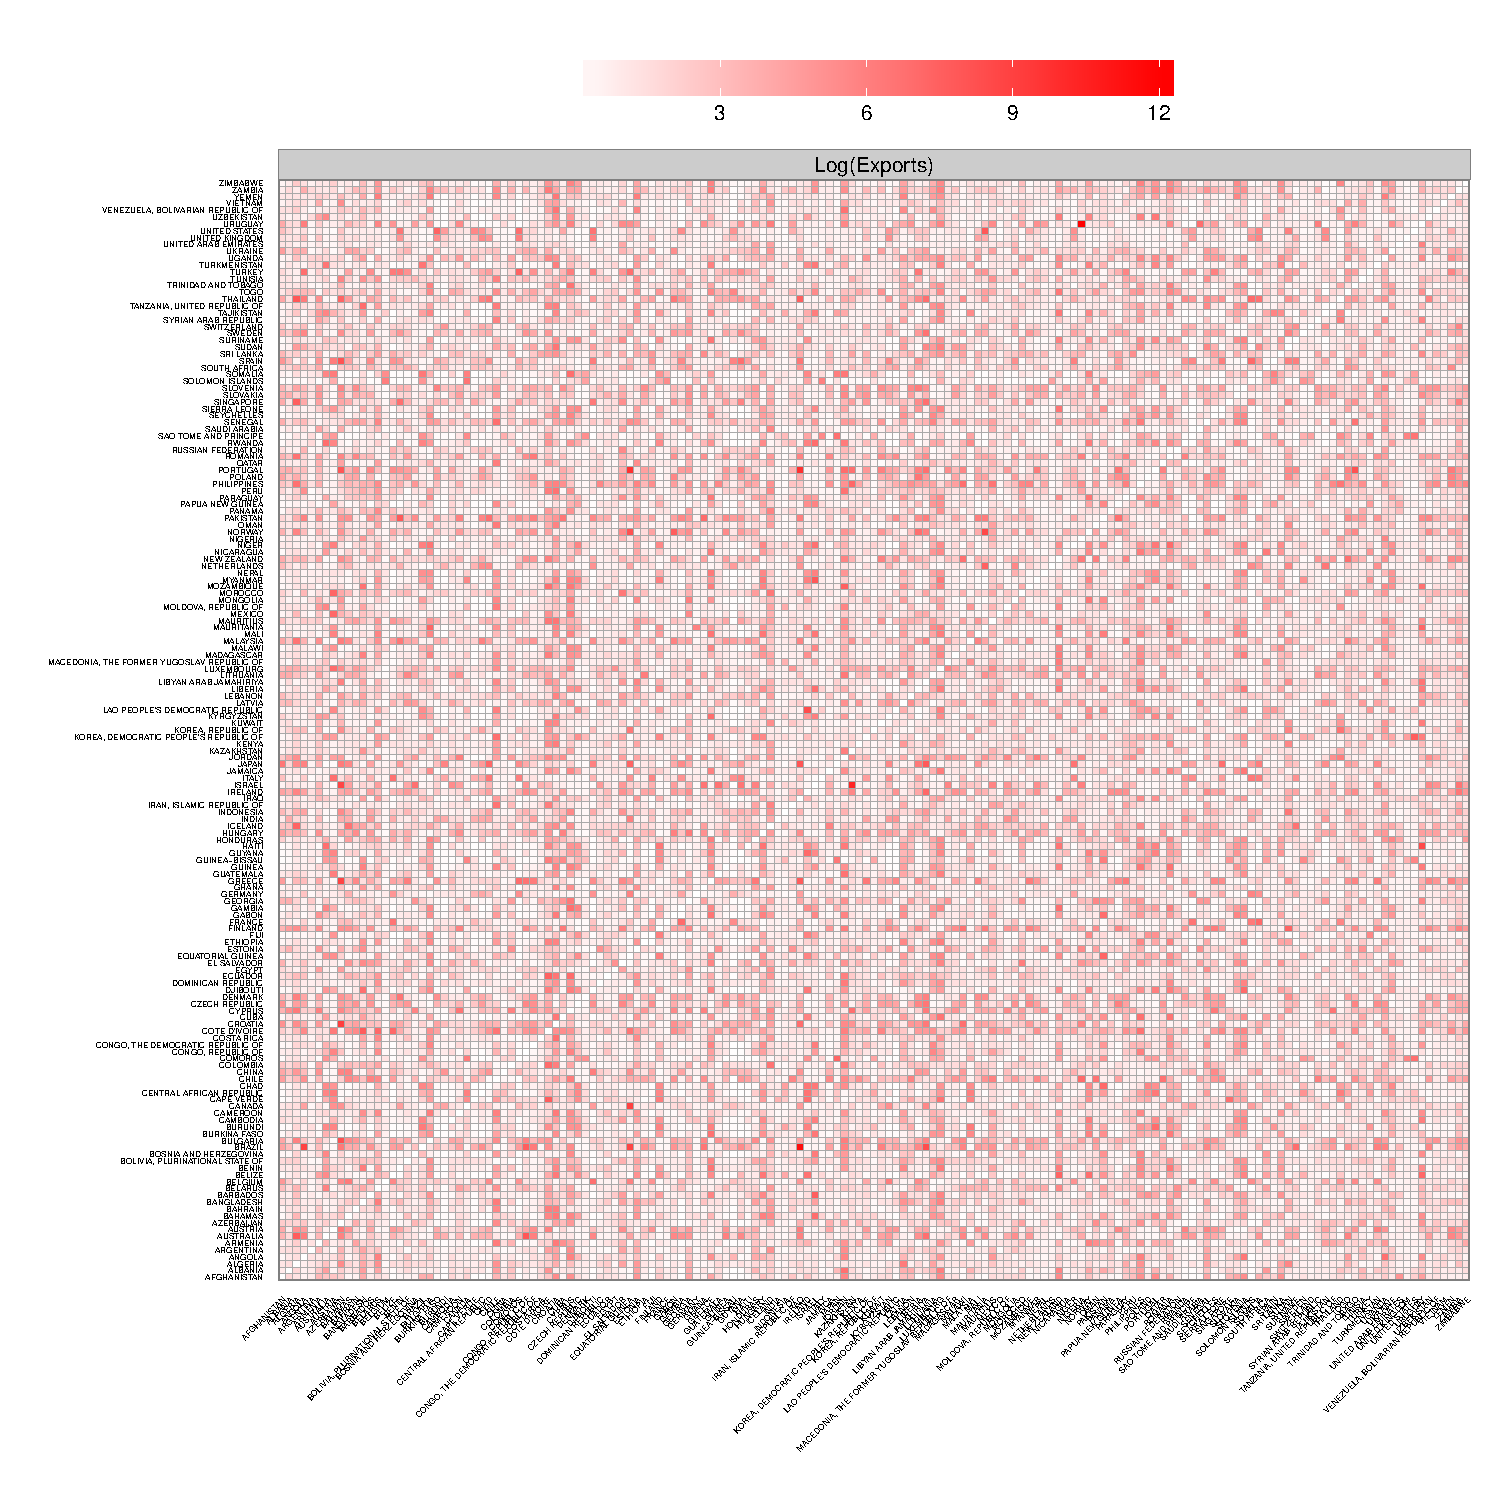
\includegraphics[width=.6\textwidth]{dyadexpiperf.pdf} & 
      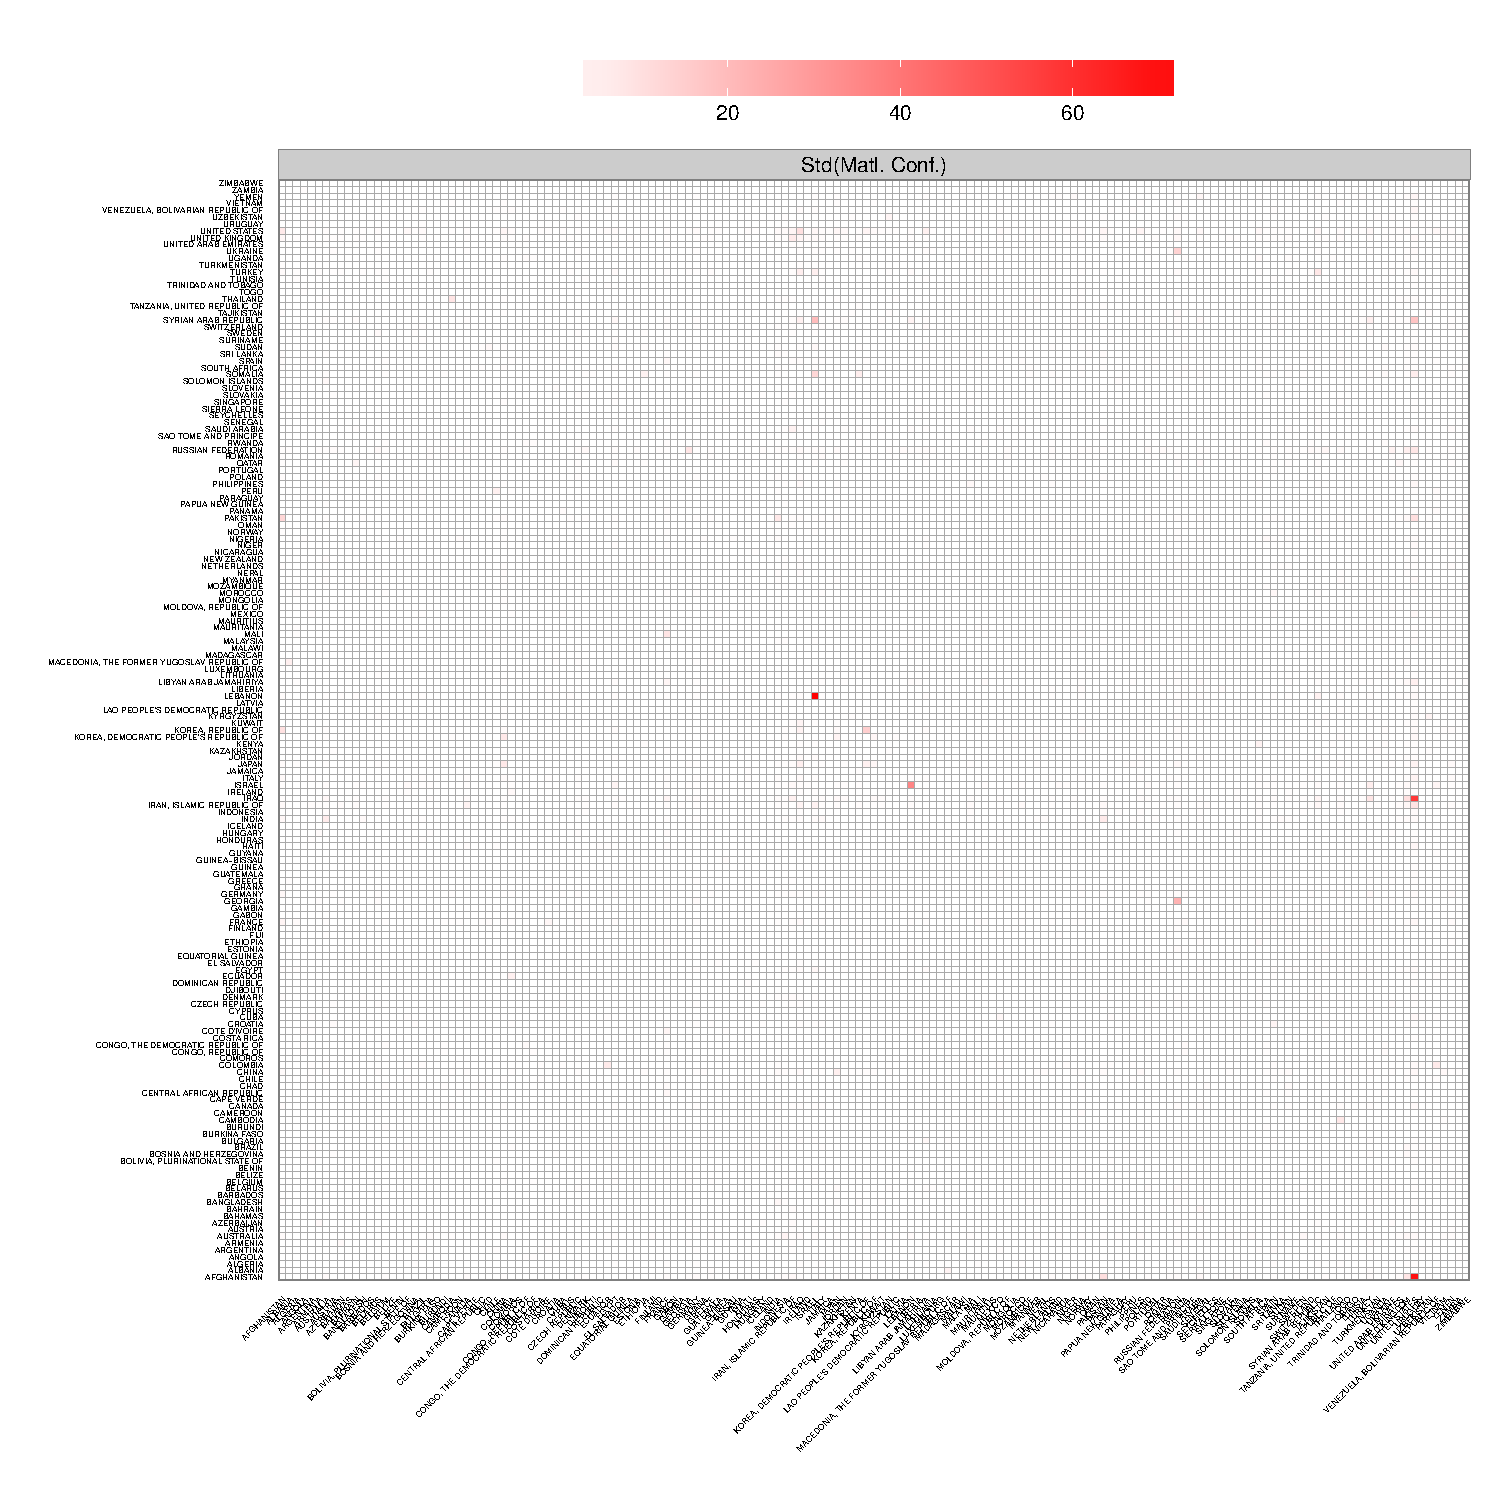
\includegraphics[width=.6\textwidth]{dyadmconfiperf.pdf}
    \end{tabular}
  \end{figure}
}
%%%%%%%%%%%%%%%%%%%%%%%%%%%%%%%%%%%%%%%%%%%%%%%%%%%%%%%%%%%%

\plain{Next Steps?}

\end{document}
